\documentclass[12pt, a4paper, twoside]{report}
\usepackage[utf8]{inputenc}
\usepackage{blindtext}
\usepackage[margin=2cm]{geometry}
\usepackage{markdown}
\usepackage[hyperref]{xcolor}
\usepackage{setspace}
\usepackage{newpxtext}
\usepackage{newpxmath}
\usepackage[margin=1cm, labelfont=bf]{caption}
\usepackage{subcaption}
\usepackage{booktabs}
\usepackage{numprint}
\usepackage{inconsolata}
\usepackage{mathtools}

\usepackage{graphicx}
\linespread{1.5}
\usepackage{xspace}
\usepackage{tikz-feynman}

\usepackage[toc,page]{appendix}

% Biblatex
\usepackage[sorting=none]{biblatex}
\bibliography{bibliography}

% Hyperlinks
\definecolor{blue1}{RGB}{50, 142, 237}
\definecolor{red1}{RGB}{239, 83, 138}
\definecolor{orange1}{RGB}{243,109,33}
%\usepackage[colorlinks=true, allcolors=blue1]{hyperref}
\usepackage[colorlinks=true, allcolors=orange1]{hyperref}
\usepackage{soul}
\usepackage{amsmath}
\usepackage{bm}
\usepackage{marginnote}
\usepackage{adjustbox}

\usepackage{sepfootnotes}

\usepackage[group-separator={,},separate-uncertainty=true]{siunitx}
\DeclareSIUnit\clight{\text{\ensuremath{c}}}

% Acronyms
\usepackage[acronym,nonumberlist]{glossaries}
\renewcommand*{\glstextformat}[1]{\textcolor{black}{#1}}
%\makeglossaries
\newacronym{COMET}{COMET}{Coherent Muon-to-Electron Conversion}

% Path of figures for each chapter
%\graphicspath{{introduction/}{chapter2/}{conclusion/}}

%
\newcommand{\diff}[2]{\frac{\textrm{d}{#1}}{\textrm{d}{#2}}}

% If table of contents goes too deep, we can limit depth.
%\setcounter{tocdepth}{0}

% Color scheme: https://coolors.co/0081a7-00afb9-fdfcdc-fed9b7-f07167

\begin{document}

% Title page
\thispagestyle{empty}
%
\includegraphics[width=0.0\textwidth]{IMP_ML_1CS_4CP.eps}


\vspace*{\fill}

\begin{center}
    
    {\huge Sensitivity Estimates and\\[-0.2cm]
    Background Study toward the \\[-0.2cm]
    COMET Phase-I Experiment \par }%Conversion Search \par}

    \vspace{1cm}
    
    {\Large Matthias Dubouchet}

    \vspace{0.8cm}
    
{\large
High Energy Physics Group\\[-0.2cm]
Department of Physics\\[-0.2cm]
Imperial College London \par
}


    \vspace{1.5cm}
    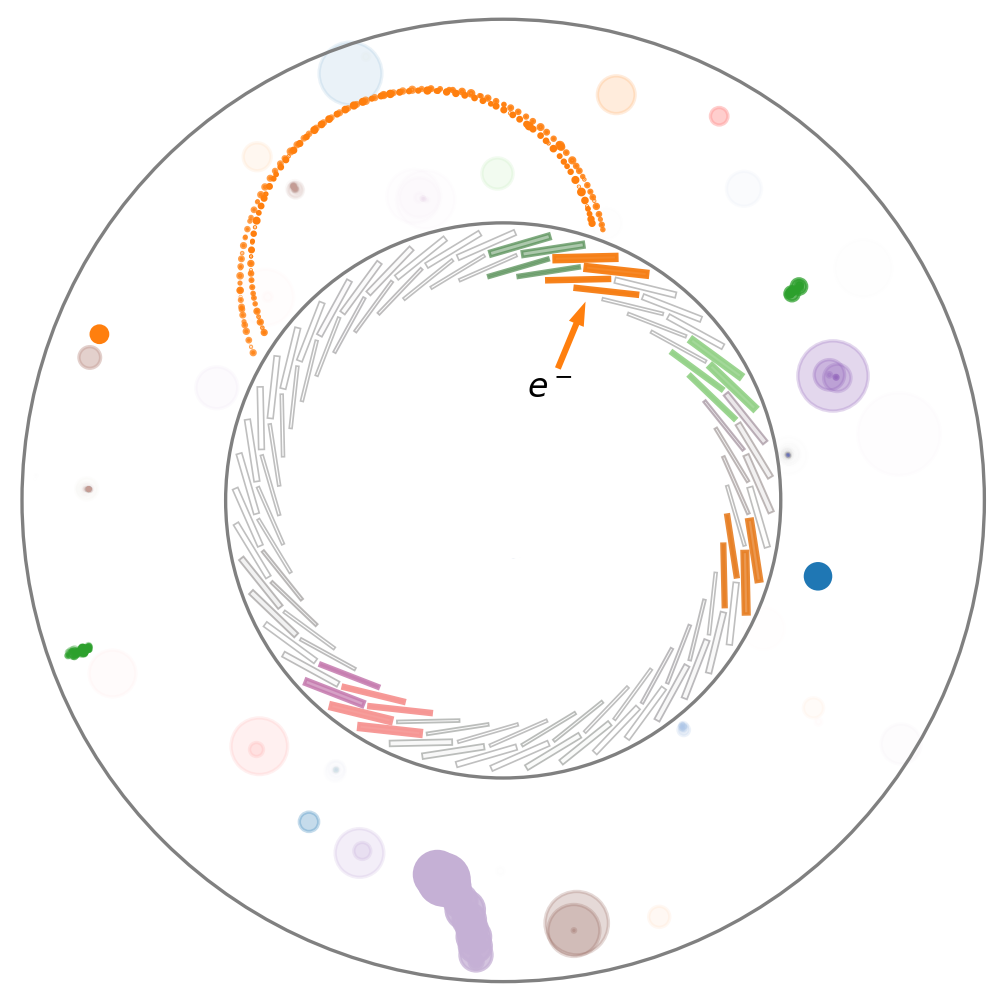
\includegraphics[width=0.35\textwidth]{title_page_graphic.png}
    \vspace{1cm}
    
    {\large Submitted in partial fulfilment of the requirements\\for the degree
    of Doctor of Philosophy}
    
\end{center}

\vspace*{\fill}
\clearpage

% Blank page
\shipout\null

\pagenumbering{roman}

\chapter*{Abstract}


COMET is a future high-precision experiment searching for charged lepton flavour
violation through the muon-to-electron conversion process. It aims to push the
intensity frontier of particle physics by coupling an intense muon beam with
cutting-edge detector technology. The first stage of the experiment, COMET
Phase\nobreakdash-I, is currently being assembled and will soon enter its data acquisition
period. It plans to achieve a single event sensitivity to $\mu$--$e$ conversion
in aluminium of $3.1 \times 10^{-15}$.

This thesis presents a study of the sensitivity and backgrounds of \mbox{COMET
Phase\nobreakdash-I} using the latest Monte Carlo simulation data produced. The background
contribution from cosmic ray-induced atmospheric muons is estimated using a
backward Monte Carlo approach, which allows computational resources to be
focused on the most critical signal-mimicking events.

Analysis of a $\mu$--$e$ conversion simulation sample suggests that COMET
Phase\nobreakdash-I will reach a single event sensitivity of $3.6 \times 10^{-15}$ within 146
days of data acquisition. In that period, the background contribution from
atmospheric muons is estimated to be 0.08 events under optimistic conditions,
namely a \SI{99.99}{\percent}-efficient Cosmic Ray Veto system and
\SI{99}{\percent} muon identification rate by the main detector.


\chapter*{Declaration}
This dissertation is the result of my own work except where explicit reference
is made to the work of others. In addition, the methods and results reported in
Section~\ref{sec:quality_metrics} were investigated by a pair of MSci students
with my guidance.

\hfill Matthias Dubouchet

\vspace{2cm}
The copyright of this thesis rests with the author. Unless otherwise indicated, 
its contents are licensed under a Creative Commons Attribution-Non 
Commercial 4.0 International Licence (CC BY-NC). 
Under this licence, you may copy and redistribute the material in any medium 
or format. You may also create and distribute modified versions of the work. 
This is on the condition that: you credit the author and do not use it, or any 
derivative works, for a commercial purpose. 
When reusing or sharing this work, ensure you make the licence terms clear to 
others by naming the licence and linking to the licence text. Where a work has 
been adapted, you should indicate that the work has been changed and 
describe those changes. 
Please seek permission from the copyright holder for uses of this work that are 
not included in this licence or permitted under UK Copyright Law.

\chapter*{Acknowledgements}

% Colleagues
I would like to thank my supervisor, Yoshi Uchida, for guiding me on this
journey. I am grateful for your teachings and the freedom I was given in
pursuing my objectives---sometimes from remote locations for extended periods of
time! Thank you also to the other members of the COMET group at Imperial, Per,
Phill, Kou and Roden, for the continuous feedback and constructive
conversations. 

Thanks to Ben and Ewen for the discussions that kickstarted my work on the COMET
experiment. I have lost count of how many times I went back to your theses to
find clarity.
To Valentin, thank you for the discussions concerning your original cosmic ray
study, from which mine is inspired in more ways than one.

And thank you to everyone from the COMET collaboration for undertaking such a
difficult project, striving to reach the best achievable outcome despite many
hurdles. It was a pleasure to discover some of your countries (and gastronomy),
and a shame that we missed a few opportunities to meet (and eat) because of the
global situation.


% Family & friends
To the members of my family, thank you for your patience and care. Florie, thank
you for proofreading this thesis, and well done managing to stay mostly awake in
the process. I am grateful, and pleasantly surprised, that you have accompanied
throughout this adventure. Thanks also to all my close friends for the moral
support and the good times.

I dedicate this work to my mother and my grandfather.



\tableofcontents
\printglossary[type=\acronymtype]
\cleardoublepage

\pagenumbering{arabic}

\chapter[Lepton Flavour in the Standard Model and Beyond]{Lepton Flavour in
the\\Standard Model and Beyond}
\label{ch:theory}

\vspace{-.4cm}

% Crazy superlatives about the SM
The Standard Model (SM) of particle physics is possibly the most successful
mathematical model of physical phenomena so far. It provides an accurate
description of almost all observable interactions between known elementary
particles. It yields predictions for what nature does and does not allow, and
enables physicists to examine and test the fundamental laws of the universe.
Furthermore, the SM establishes a rigid framework to make theoretical
predictions, from which any measured deviations can then be interpreted as new
physics.

The conservation of lepton flavour, which stems from an accidental symmetry of
the SM, is currently under strict scrutiny by various experiments around the
world. The observation of neutrino oscillations has already proven that lepton
flavour is not conserved by neutral leptons, and this has further driven the
search for lepton flavour violation among the charged leptons. If charged lepton
flavour violation (CLFV) is observed, not only would it be paradigm-shifting
evidence for physics beyond the Standard Model, but it will also help guide us
toward the next theory of particle physics by hinting at the underlying
processes which could be at play.

The most sensitive probe to search for charged lepton flavour violation is the
muon, in large part because muons can be readily produced and focused into
intense beams at accelerator facilities. This chapter describes how the muon has
come from being a mysterious particle showering Earth from high in the
atmosphere to becoming a tool in high energy physics experiments used to explore
the frontier of our knowledge of nature.


\section{Discovery of the muon}
The first traces of muons were observed around 1937 by three experiments
investigating the nature of cosmic ray-induced particle
showers~\cite{PhysRev.51.884, PhysRev.52.1198, PhysRev.52.1003}. One of them was
able to estimate the mass of the discovered particle at hundreds of times that
of the electron: around the same as the strong-force-carrying meson predicted by
Yukawa in 1935~\cite{10.1143/PTPS.1.1}. Hence, the muon and Yukawa's particle
were originally believed to be one and the same particle. 

It was only a decade later, when the meson (now called $\pi$, for primary) was
observed decaying into a muon, that the two particles were completely
disambiguated. The discovery of the pion was attributed to the
Lattes--Muirhead--Occhialini--Powell group~\cite{LATTES1947}, but it was Don
Perkins, doctoral student at Imperial College London at the time, who recorded
the first nuclear emulsion of a negative pion capture and set in motion the race
to identify this new particle~\cite{vieira_carried_2014}.

Subsequently, it was the fact that the muon appeared as nothing but a heavy
electron which prompted Rabi to ask ``who ordered that?'' in response to its
discovery. In fact, even the Standard Model of today remains unable to give a
satisfactory answer to this question, since the SM does not motivate the
existence of three generations of elementary particles. As far as the SM can
explain, there is no fundamental reason for the existence of distinct flavours.

\section{The muon in the Standard Model}

The SM identifies the muon as the second-generation charged lepton, meaning it
is a fermion with identical properties, aside from flavour and mass, as the electron
and tau lepton. A muon in a vacuum can only decay through the weak force. The
diagram for muon decay, $\mu^- \rightarrow e^- +  \nu_\mu + \overline{\nu}_e$,
is shown in Figure~\ref{fig:weak_decay}.

\begin{figure}
    \centering
    \feynmandiagram [layered layout, horizontal=a to b] {
        a [particle=\(\mu^{-}\)] -- [fermion] b -- [fermion] f1 [particle=\(\nu_{\mu}\)],
        b -- [boson, edge label'=\(W^{-}\)] c,
        c -- [anti fermion] f2 [particle=\(\overline \nu_{e}\)],
        c -- [fermion] f3 [particle=\(e^{-}\)]
    };

    \caption{ Feynman diagram for the weak decay of the muon. Note how lepton
        flavour is conserved by the presence of a muon neutrino and an electron
        anti-neutrino. }
    \label{fig:weak_decay}
\end{figure}

In the SM Lagrangian with massless neutrinos, none of the terms which involve
leptons allow for flavour violation. The Lagrangian is invariant under
transformations of the ${U(1)_e \times U(1)_\mu \times U(1)_\tau}$ group.
Consequently, each lepton generation ($e$, $\mu$, $\tau$) has its own conserved
number. In theory, this completely prevents a charged lepton from changing
flavour without neutrinos being involved to balance the process. 

These conservation laws do not correspond to a fundamental symmetry of nature;
they are merely an accidental feature of the SM Lagrangian and have, so far,
been observed to hold experimentally. 
For instance, the process ${\mu \rightarrow e + \gamma}$, in principle allowed
by kinematics, has never been observed and the current upper limit on its
branching ratio was set by the MEG experiment at
$10^{-13}$~\cite{mori2016final}. 



\subsection{Tensions between theory and experiment}
Various fundamental properties of the muon are currently under investigation by
experiments around the world. Recent measurements have started to suggest that
the charged lepton sector might be the next to reveal physics beyond the
Standard Model (BSM). From only these results, predicting whether CLFV will also
appear is not possible. However, CLFV searches are complementary in constraining
the models of new physics which could lead to the observed discrepancies.

The Muon $g-2$ experiment at Fermilab recently observed a $4.2\sigma$
discrepancy between the Standard Model prediction and the measured value for the
magnetic moment of the muon~\cite{PhysRevLett.126.141801}. This deviation,
assuming it is a true sign of new physics\footnote{
    The theoretical expectation for the SM magnetic moment is disputed by a
    different approach using lattice QCD~\cite{Borsanyi2021}. The latter calculation
    is indeed more consistent with the measurement, hence further investigation is
    necessary to understand the cause of the initial discrepancy and why the two
    calculations disagree.
}, could be attributed to various scenarios where new particles, e.g.\ 
leptoquarks, a new Higgs doublet or neutral boson, interact with the muon.


The LHCb experiment at CERN has found evidence for lepton non-universality in
the decay of b-quarks, with a significance of $3.1\sigma$~\cite{Aaij2022}. As
with the $g-2$ discrepancy, models which could explain the anomaly include a
heavy neutral boson, leptoquarks, or an extended Higgs sector. 

Together, the Muon $g-2$ and LHCb tensions suggest a special property of the
muon which would differentiate it from the electron in a new, so far unexplained
way. Although there are so far no tangible traces of CLFV, theoretical models
attempting to resolve the $g-2$ and LHCb anomalies often also allow CLFV at a
level within experimental reach~\cite{DEGOUVEA201375, PhysRevD.101.115016,
PhysRevD.100.115010}. Hence, measurements such as the $\mu$--$e$ conversion
branching ratio are crucial to further constrain models and guide the theory
toward the true nature of the new physics.


% CLFV with neutrino oscillations: GIM suppression
\subsection{Lepton flavour with massive neutrinos}
The observation of neutrino oscillations~\cite{PhysRevLett.81.1562} means that
the three accidental lepton flavour symmetries are not exact. It is now known
that the flavour content of a neutrino changes as it propagates, hence the
flavour quantum numbers are not true conserved quantities for leptons. 

In the quark sector, flavour-changing neutral currents (FCNC) are one-loop order
processes which allow a quark to change generations (e.g.\ from a strange quark
to a down quark). The small rates of such processes are explained by the GIM
(Glashow--Illiopoulos--Maiani) mechanism: interference between diagrams with
different flavours of mediating quarks causes the branching ratio of FCNC to be
heavily suppressed~\cite{PhysRevD.2.1285}.




\begin{figure}
\centering
\begin{subfigure}[t]{0.45\textwidth}
    \centering
    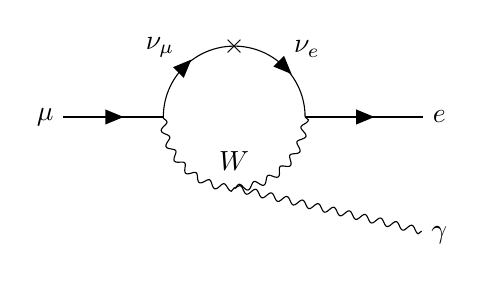
\begin{tikzpicture}
    \begin{feynman}
    \vertex (a) {\(\mu\)};
    \vertex [right=1.5cm of a] (b);
    \vertex [right=1.8cm of b] (c);
    \vertex [right=1.5cm of c] (d) {\(e\)};
    
    \vertex at ($(b)!0.5!(c) + (0, 0.9cm)$) (n);
    \vertex at ($(b)!0.5!(c) + (0, -0.9cm)$) (w);
    \vertex [above=0.1cm of w] (wn) {\(W\)};
    \vertex [below=1.5cm of d] (g) {\(\gamma\)};
    
    \diagram* {
    (a) -- [fermion] (b)
    -- [fermion, quarter left, edge label=\(\nu_\mu\)] (n)
    -- [fermion, quarter left, edge label=\(\nu_e\)] (c),
    (b) -- [boson, quarter right] (w)
    -- [boson, quarter right] (c),
    (c) -- [fermion] (d),
    (w) -- [boson] (g),
    };
    
    \draw (n) -- (n) node {\(\times\)};
    
    \end{feynman}
    \end{tikzpicture}
    \caption{
        $\mu \rightarrow e + \gamma$
    }
    \label{fig:mu_e_nu_osc}
\end{subfigure}
\begin{subfigure}[t]{0.45\textwidth}
    \centering
    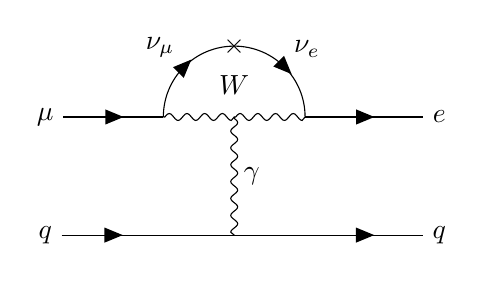
\begin{tikzpicture}
    \begin{feynman}
    \vertex (m1) {\(\mu\)};
    \vertex [right =1.5cm of m1] (m2);
    \vertex [right =1.8cm of m2] (m3);
    \vertex at ($(m2)!0.5!(m3)$) (w);
    \vertex at ($(m2)!0.5!(m3) + (0, 0.4cm)$) (wl) {\(W\)};
    \vertex at ($(m2)!0.5!(m3) + (0, 0.9cm)$) (n);
    \vertex [right =1.5cm of m3] (m4) {\(e\)};

    \vertex [below =of m1] (q1) {\(q\)};
    \vertex [below =of m2] (q2);
    \vertex [below =of m3] (q3);
    \vertex [below =of m4] (q4) {\(q\)};
    \vertex at ($(q2)!0.5!(q3)$) (qg);
    
    \diagram* {
    (m1) -- [fermion] (m2)
    -- [fermion, quarter left, edge label=\(\nu_\mu\)] (n)
    -- [fermion, quarter left, edge label=\(\nu_e\)] (m3),
    (m2) -- [boson] (w)
    -- [boson] (m3)
    -- [fermion] (m4),
    (q1) -- [fermion] (q2)
    -- (q3)
    -- [fermion] (q4),
    (w) -- [boson, edge label=\(\gamma\)] (qg),
    };

    \draw (n) -- (n) node {\(\times\)};
    
    \end{feynman}
    \end{tikzpicture}
    \caption{
        $\mu+N \rightarrow e + N$
    }
    \label{fig:mu-e_conv_SM}
\end{subfigure}
    \caption{
        Feynman diagrams of processes allowing charged lepton flavour
        violation in the SM extended with neutrino masses. Although these
        processes enable CLFV, their branching ratios are heavily suppressed to
        unobservable levels because of the lightness of
        neutrinos compared to the weak scale~\cite{BERNSTEIN201327}.}
    \label{fig:lepton_fcnc}
\end{figure}

In the lepton sector, the fact that neutrinos are massless in the SM implies
that FCNC among charged leptons is completely forbidden. With the addition of
massive oscillating neutrinos, processes such as those shown in
Figure~\ref{fig:lepton_fcnc} become allowed. These provide the only currently
known way that charged lepton flavour can be violated. However, the GIM
suppression in this case is much more significant than in the quark sector
because neutrinos are almost massless (compared to the weak scale). For
instance, oscillating neutrinos allow the process shown in
Figure~\ref{fig:mu_e_nu_osc} to occur, which gives rise to a non-zero rate for
${\mu \rightarrow e + \gamma}$. The branching ratio calculated for this process
using the upper limit on neutrino masses is given by~\cite{BERNSTEIN201327}
\begin{equation}\label{eq:br_meg}
\mathcal{BR}(\mu \rightarrow e + \gamma) = \frac{3\alpha}{32\pi} \left|\ \sum_{i=2, 3} U^*_{\mu i} U_{e i} 
\frac{\Delta m^2_{i1}}{m^2_W}  \ \right| ^2 \approx 10^{-54},
\end{equation}
where $U$ is the PMNS matrix, $\Delta m^2_{ij}$ is the mass-squared difference
between the $i$-th and $j$-th neutrino mass eigenstates, and $m_W$ is the
$W$-boson mass. 
A similar suppression also applies to the rates of other muon CLFV processes allowed in the
SM extended with neutrino masses~\cite{doi:10.1063/1.56214}.

The vanishingly small branching ratio of Equation~\ref{eq:br_meg} implies that
$\mu\rightarrow e\gamma$ cannot be observed experimentally unless some
unexpected interaction is at play. Consequently, this and other CLFV processes
are excellent probes to search for new physics. Specifically, many models for
BSM physics give rise to direct mixing between charged lepton flavours at levels
that may be observable in current and near-future experiments. Any experimental
evidence that CLFV occurs at a rate higher than that of a neutrino-mediated FCNC
would yield important clues as to what new physics lies beyond the SM.

\section{Searching for charged lepton flavour violation}\label{sec:clfv}

Three muon processes can be investigated in order to search for CLFV: ${\mu
\rightarrow e\gamma}$, ${\mu \rightarrow eee}$ and ${\mu N \rightarrow e N}$
(muon-to-electron conversion)~\cite{BERNSTEIN201327}. Observing any one of them
would fundamentally contradict the Standard Model and thus provide undeniable
evidence for a new interaction. Then, observing a second CLFV process would help
us to determine which of the many theorised models for new physics is realised
in nature. 


\begin{figure}
    \centering
    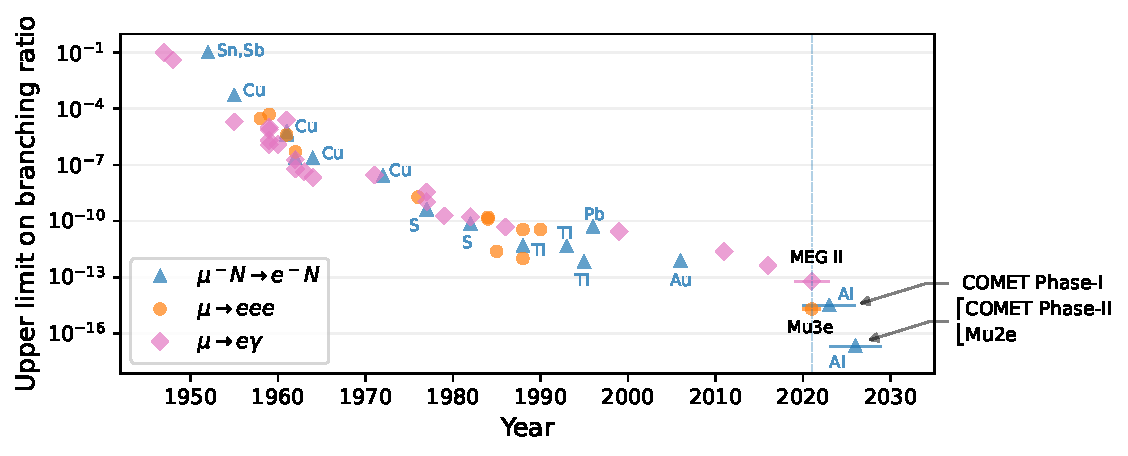
\includegraphics[width=\linewidth]{chapter1/clfv_upper_limit_v2.pdf}\hspace{-1.5cm}
    \caption{
    90\%-confidence upper limit on the branching ratio of three charged lepton
    flavour-violating processes over time. The target material $N$ is indicated
    for $\mu$--$e$ conversion experiments. Past experiment results were
    tabulated in Reference~\cite{BERNSTEIN201327}. Future data points are the
    expected sensitivities quoted in the MEG II~\cite{Baldini2018},
    Mu3e~\cite{ARNDT2021165679}, COMET
    Phase-I~\cite{the_comet_collaboration_comet_2020} and
    Mu2e~\cite{bartoszek2015mu2e} design reports.
    }
    \label{fig:clfv_upper_limit}
\end{figure}

CLFV has been sought after ever since the muon's discovery: the first
investigation of whether nature allows $\mu \rightarrow e \gamma$ was performed
in 1948~\cite{PhysRev.73.257}. A multitude of experiments followed, but none so
far have been able to find a signal~\cite{BERNSTEIN201327}.
Figure~\ref{fig:clfv_upper_limit} shows experimentally-estimated upper limits on
the branching ratios of $\mu \rightarrow e\gamma$, $\mu\rightarrow eee$ and $\mu
N \rightarrow e N$ over time, since the first experiment and into the next
decade. 

As higher and higher sensitivities are required, experiments must be able to
produce a muon source which is increasingly intense while demonstrating
precise control over every source of background. This is made possible by new
technologies in both hardware and software applied across entire experiment
designs. The next generation of CLFV-seeking precision experiments, which
consists of MEG II, Mu3e, COMET and Mu2e, aims to be 10 to \numprint{10000}
times more sensitive than the last generation.


\section{Muon-to-electron conversion}
% mu-e conversion
Muon-to-electron conversion is the neutrino-less decay of a muon bound to an
atomic nucleus:
\begin{equation}
\mu^- + N(A, Z) \rightarrow e^- + N(A, Z),
\end{equation}
where $A$ is the mass number and $Z$ the atomic number.
Similarly to $\mu\rightarrow e\gamma$, this process is allowed in the SM
extended with massive neutrinos via the diagram shown in
Figure~\ref{fig:mu-e_conv_SM}, but suppressed to an experimentally
unreachable level. Any signs of it occurring at current experimental
sensitivities would suggest a BSM origin.

In order to search for this process, muons must be stopped in matter to form
muonic atoms. Initially bound in the outer atomic layers, the muon
electromagnetically cascades down to the $1s$ orbital within close range of the
nucleus over the following nanosecond~\cite{Knecht2020}. When interacting with
the nucleus, the reaction is called \emph{coherent} if the nucleus remains
unchanged and in its ground state. For elements heavier than magnesium, the
ratio of coherent to incoherent $\mu$--$e$ conversion is expected to be around
9:1~\cite{CHIANG1993526}.

In a coherent $\mu$--$e$ conversion, the kinematics are those of a
straightforward two-body decay, hence the electron always has an energy
\begin{equation}\label{eq:mu_e_conv_energy}
E_{\mu\text{--}e} = m_\mu - B_\mu - E_\mathrm{recoil},
\end{equation}
where $B_\mu$ is the binding energy of the $1s$-state muonic atom and
$E_\mathrm{recoil}$ is the recoil energy of the nucleus. In aluminium, the
target material of the COMET and Mu2e experiments, this yields

\begin{equation}
    E^\mathrm{Al}_{\mu\text{--}e} = \SI{104.97}{\MeV}.
\end{equation}
Since the signature of $\mu$--$e$ conversion is a single, mono-energetic
electron, this process should be relatively easily identified by means of a
momentum-measuring detector. However, this signal must also be discriminated
from backgrounds originating from other processes, contamination of the beam and
cosmic rays.

\subsection{Standard Model backgrounds}\label{sec:sm_backgrounds}

\begin{figure}
    \centering
    \begin{subfigure}[t]{0.47\textwidth}
        \hspace{-.5cm}
        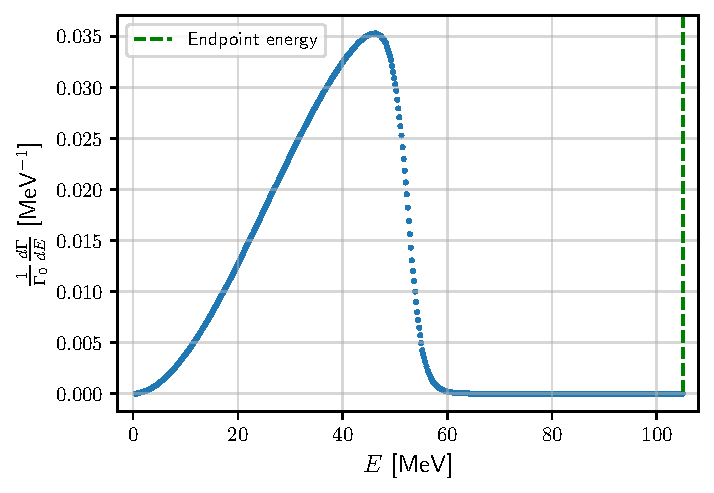
\includegraphics[width=\textwidth]{chapter1/dio_spectrum_lin.pdf}
        \caption{Linear vertical axis.}
    \end{subfigure}
    \hfill
    \begin{subfigure}[t]{0.47\textwidth}
        \hspace{-.5cm}
        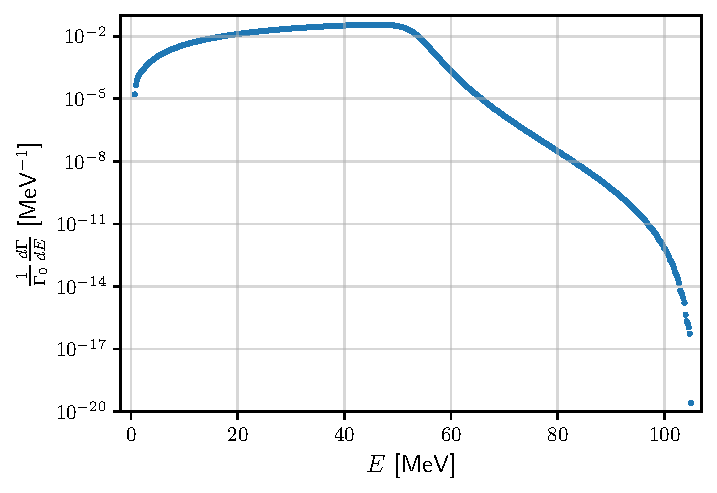
\includegraphics[width=\textwidth]{chapter1/dio_spectrum_log.pdf}
        \caption{Logarithmic vertical axis.}
    \end{subfigure}
    \caption{Energy spectrum of decay-in-orbit electrons produced by muonic
    aluminium atoms, calculated by Czarnecki et al.~\cite{czarnecki}. The
    logarithmic scale reveals the shape of the high-energy tail up to the
    endpoint energy of \SI{104.97}{\MeV}.}
    \label{fig:dio_energy_spectrum}
\end{figure}


\subsubsection{Decay in orbit}
In the SM, a bound muon is allowed to decay in orbit (DIO):
\begin{equation}\label{eq:dio}
    \mu^- + N(A, Z) \rightarrow e^- + \nu_\mu + \overline{\nu}_e + N(A, Z).
\end{equation}
Although the process is the same as a free decay, shown in
Figure~\ref{fig:weak_decay}, here the nucleus is also involved in the kinematics
of the process. In a free decay, the electron may carry at most half of the muon
mass as kinetic energy (in the muon rest frame) when the two neutrinos are
emitted in the opposite direction. In DIO, the nucleus can recoil and
potentially provide more energy to the electron. If the two neutrinos are
emitted back to back in the transverse direction to the electron, then the
kinematics resemble that of $\mu$--$e$ conversion and the electron could easily
be mistaken for the CLFV signal. 

% Mention muon lifetime in orbit?

The energy spectrum of DIO electrons for various target nuclei is well
understood theoretically~\cite{czarnecki}, hence the expected background rate
for $\mu$--$e$ conversion searches can be estimated. The DIO energy spectrum for
aluminium is shown in Figure~\ref{fig:dio_energy_spectrum}. Although it is
highly unlikely that a DIO electron might carry as much energy as a conversion
electron, DIO remains one of the main sources of background because of the
extreme sensitivity aimed at by upcoming $\mu$--$e$ conversion searches, as well
as the finite resolution achievable by the detectors given the high-intensity
environment~\cite{the_comet_collaboration_comet_2020}. These effects are
illustrated in Figure~\ref{fig:signal_dio_momentum_spectrum_tdr}, which shows
the expected momentum distributions for conversion and DIO electron tracks in
COMET Phase\nobreakdash-I.


\subsubsection{Nuclear capture}
A muon in proximity with a nucleus may also be captured via $W$-boson exchange:
\begin{equation}\label{eq:capture}
    \mu^- + N(A, Z) \rightarrow \nu_\mu + N(A, Z-1).
\end{equation}
This process is similar to an electron capture and transmutes the nucleus into a
potentially unstable isotope, which can be the source of proton, photon and
neutron emissions as it readjusts. Particles emitted by the nucleus after muon
capture may fly into the detector system and cause unwanted occupancy of the
readout. This is especially concerning if the detector is close to the target,
as is the case in Phase\nobreakdash-I. Hence, the AlCap experiment was performed in 2013 at
the Paul Scherrer Institute to measure the spectrum and yield of particles
emitted after capture of stopped muons by aluminium
nuclei~\cite{PhysRevC.105.035501}. The yield of highly-ionising particles was
found to be half as much as the previous expectation, deduced from observations
of nuclear capture by silicon nuclei, and the amount of detector shielding
required in the Phase\nobreakdash-I design was subsequently reduced.

\begin{figure}
    \centering
    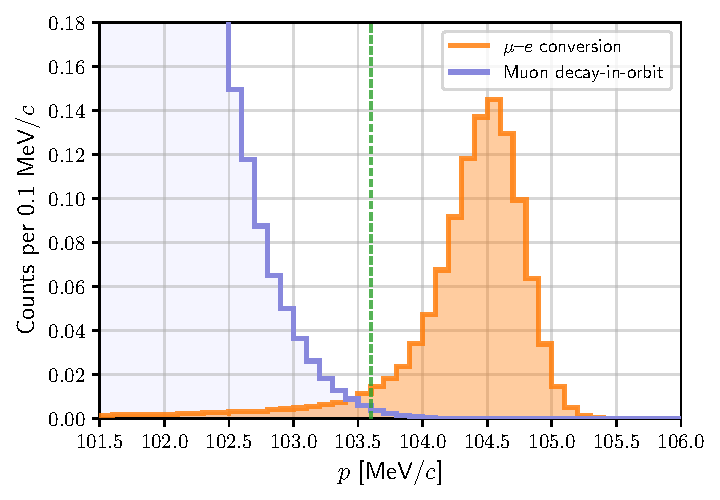
\includegraphics[width=0.6\textwidth]{chapter1/signal_dio_momentum_spectrum.pdf}
    \caption{ Momentum distribution of reconstructed signal and decay-in-orbit
        electrons in COMET Phase-I, assuming a conversion branching ratio of
        $3\times 10^{-15}$. A momentum resolution of
        \SI{200}{\keV/\clight} is assumed, and detector efficiency factors are
        extracted from the technical design
        report~\cite{the_comet_collaboration_comet_2020}. The vertical dashed
        line shows the lower bound of the momentum window at
        \SI{103.6}{\MeV/\clight}, which is used to discriminate background
        events from the conversion signal. }
    \label{fig:signal_dio_momentum_spectrum_tdr}
\end{figure}

Radiative muon capture (RMC) occurs when a photon is emitted during the capture
process. Kinematically, the photon can carry energies close to the muon mass.
Hence, if it goes on to produce an electron--positron pair with asymmetric
momenta, the electron will mimic the conversion signal. The high-energy endpoint
of the RMC spectrum is not as high as for DIO, hence an adequate momentum
resolution from a tracking detector will discriminate most RMC electrons from
the signal. In COMET Phase\nobreakdash-I, the expected background count from RMC is 5 times
lower than that from DIO~\cite{the_comet_collaboration_comet_2020}.




Sources of background other than DIO and nuclear capture are expected in
$\mu$--$e$ conversion-searching experiments, such as beam-related and cosmic
ray-induced events. All backgrounds specific to the COMET experiment, and the
associated design choices which were made to minimise their occurrence, are
discussed in Section~\ref{sec:backgrounds}.






\section{Effective CLFV and the scale of new physics}
Experiments searching for CLFV are sensitive to a wide variety of new physics,
including a non-minimal Higgs, a $Z'$ boson, leptoquarks, heavy neutrinos, and
supersymmetric particles. 
In order to determine the scale of new physics to which future CLFV-searching
experiments will be sensitive and the complementarity between experiments, we can
consider a low-energy effective field theory derived from new interactions with
generic massive ($m>\SI{1}{\tera\eV}$) particles.
After integrating out heavy fields (see
e.g.~\cite[Chapter~IV]{donoghue_golowich_holstein_2014}), one obtains the
following effective Lagrangian~\cite{DEGOUVEA201375}, which allows CLFV to be
mediated by the tree-level vertices shown in Figure~\ref{fig:tree_lvl_clfv}:
\begin{align}\label{eq:Leff}
    \mathcal{L^\text{eff}_\mathrm{CLFV}}\,
    =\,
    &\frac{1}{\kappa+1}\, \frac{m_\mu}{\Lambda^2}\,\,
    \overline{\mu}_R \sigma_{\mu\nu} e_L \, F^{\mu\nu} + \text{h.c.}
    \nonumber\\[1em]
    +\,
    &\frac{\kappa}{\kappa+1}\, \frac{1}{\Lambda^2}\,\,
    \overline{\mu}_L \gamma_\mu e_L \,
    (\,
        \overline{u}_L \gamma^\mu u_L + \overline{d}_L \gamma^\mu d_L
    \,) + \text{h.c.}
\end{align}
where both interactions are suppressed by factors of $\Lambda$, the energy scale
of the new physics, and $\kappa$ determines whether the preferred channel is
photonic ($\kappa \rightarrow 0$) or four-fermionic ($\kappa \rightarrow
\infty$). The $\kappa$ parameter allows this Lagrangian to
be model-independent, i.e.\ it gives freedom for the new interaction to either
enhance $\mu \rightarrow e\gamma$ or $\mu$--$e$ conversion more strongly.
Searches for $\mu \rightarrow e\gamma$ will be more sensitive to CLFV than
$\mu$--$e$ conversion searches if $\kappa \ll 1$, whereas the opposite is true
if $\kappa \gg 1$.

\begin{figure}
    \centering
    \begin{subfigure}[b]{0.3\textwidth}
        \centering
        \feynmandiagram [small, inline=(b.base), vertical=b to d] {
            a [particle=\(\mu^{-}\)] -- [fermion] b [blob]
            -- [fermion] c [particle=\(e^-\)],
            b -- [boson] d [particle=\(\gamma\)],
        };
        \caption{Photonic}
    \end{subfigure}
    \hspace{1cm}
    \begin{subfigure}[b]{0.3\textwidth}
        \centering
        \feynmandiagram [small, inline=(b.base), vertical=a to d] {
            a [particle=\(\mu^{-}\)] -- [fermion] b [blob]
            -- [fermion] {c [particle=\(e^-\)],
            e [particle=\(q\)]},
            d [particle=\(q\)] -- [fermion] b,
        };
        \caption{Four-fermionic}
    \end{subfigure}
    \caption{New vertices which arise in the effective Lagrangian of
    Equation~\ref{eq:Leff} and allow CLFV. The photonic interaction can also mediate
    $\mu$--$e$ conversion by making the photon interact with an external quark.}
    \label{fig:tree_lvl_clfv}
\end{figure}

From the estimated sensitivity of a future experiment, we can estimate the
maximum scale of new physics $\Lambda$ which the experiment will be able to
probe. COMET Phase\nobreakdash-II and Mu2e, which have a single-event
sensitivity of around $10^{-17}$~\cite{the_comet_collaboration_comet_2020,
bartoszek2015mu2e}, will probe energy scales $\Lambda$ up to \SI{4000}{\tera\eV}
if $\kappa$ is small, and up to \SI{7000}{\tera\eV} if $\kappa$ is
large~\cite{ben_thesis, ewen_thesis}. 

Even in the situation where no positive signal is observed, probing these enormous
energy scales will heavily constrain any model which predicts new heavy
particles whose interactions allow any significant amount of CLFV. On the other
hand, if CLFV is observed in either the $\mu\rightarrow e\gamma$ or $\mu$--$e$
conversion channels, the value of $\kappa$ can then be determined from a
measurement in the other channel. This data will then further constrain and
disambiguate models, and help to pinpoint the true nature of the new physics.

\chapter{The COMET Experiment}\label{ch:comet}

% \begin{markdown}
% ---

% - Description of the COMET experiment's goal, design with nice illustrations
%     + Signal and background:
%         + mu-e conv signal description
%         + **List of background sources**
% + CyDet:
%     + For simulation section, need to explain how CDC and CTH work, and how
%       combined they enable mu--e conv measurement
%     - Detailed description of the CDC, which is crucial for the GAN section.
%      - Stereo angles
% + Phase alpha?

% - References: TDR, SINDRUM II, 

% ---

% + Requirements: high sensitivity to signal, efficient rejection of backgrounds
%  + -> Need intense muon beam, pulsed, and detector design must avoid
%    backgrounds
% + TIMING of signal (muon lifetime)
% + Proton beam energy: why 8 Gev -> antiproton production
% + Intensity: beam current, beam power, POTs per second
% + Send backward-going secondaries to detector, discard the main part of
%   secondaries (forward-going)
% + Curved solenoid + dipole field (by tilting coils, see Krikler)
% + Stopping target -> why Al
% + Bunch structure, extinction
% + Phase-I detectors: StrECAL and CyDet

% ---
% \end{markdown}

% Description and goals
COMET (COherent Muon-to-Electron Transition) is a future muon-beam experiment
designed to search for the muon-to-electron conversion
process~\cite{the_comet_collaboration_comet_2020}. It is currently under
construction at the Japan Proton Accelerator Research Complex (J-PARC) facility
in Tokai, Japan. The goal of COMET is to be \numprint{10000} times more
sensitive to $\mu$--$e$ conversion than the current world-leading limit set by
the SINDRUM II experiment~\cite{Bertl:2006up}. 

\subsubsection{Requirements}
In order to reach its goal, the COMET experiment is designed with strict
requirements defined to make the conversion signal as clear as possible, while
efficiently rejecting background events. The essential requirements that define
the COMET experiment are:
\begin{itemize}
    \item An intense muon source to probe the rare conversion process;
    \item A pulsed beam such that timing information can be used to reject
    backgrounds;
    \item Strict selection of charge and momentum of beam particles prior to
    reaching the detector;
    \item A tracking detector to search for the \SI{104.97}{\MeV} conversion
    signature.
\end{itemize}
These requirements and the design choices that were made to address them are
described in more detail in the rest of this chapter.

\subsubsection{Strategy}
COMET is planned to run in a staged approach such that the properties of the
newly designed beam can be finely understood before making the measurement.
COMET Phase-I has a double purpose, each fulfilled by a distinct detector
system. The StrECAL detector, composed of a straw-tube tracker and
electromagnetic calorimeter, will study the beam composition and timing
properties and increase our understanding of potential backgrounds. The
Cylindrical Detector, composed of a cylindrical drift chamber and a trigger
hodoscope, will be used to perform a $\mu$--$e$ conversion search with a
single-event sensitivity (see Section~\ref{sec:SES}) of $3\times 10^{-15}$, a
factor-100 improvement over SINDRUM II. COMET Phase-II is a planned upgrade to
Phase-I with higher beam intensity and better background rejection via a longer
momentum-selecting beamline. Phase-II aims to improve on the single-event
sensitivity of Phase-I by another factor $100$ to reach a single event
sensitivity of $2.6\times 10^{-17}$.

\subsubsection{Design}
Figure~\ref{fig:comet_schematic} shows a top-down schematic view of the COMET
experiment, laying out the different sections that make up the beamline in
Phase-I and Phase-II. In the latter, the transport solenoid is doubled to allow
more pions to decay into muons while tightening the momentum selection further.
An additional curved solenoid, the \emph{electron spectrometer,} further
eliminates particles whose momenta do not match the \SI{104.97}{\MeV} conversion
signature before they enter the detector system. While Phase-I will use the
StrECAL to study the beam properties, Phase-II will use it as the
conversion-searching detector system.\\
The following sections describe in more detail each component of the COMET
beamline.

\begin{figure}
    \centering
    \begin{subfigure}[b]{0.46\textwidth}
    \centering
        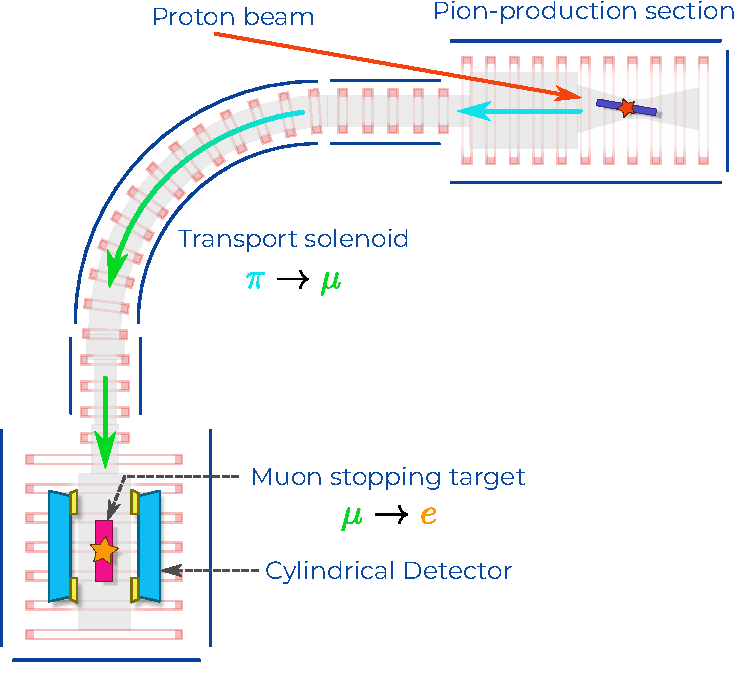
\includegraphics[width=\textwidth]{chapter2/comet_schematic_phase-I.pdf}
        \vspace{3cm}
        \caption{Phase-I with the Cylindrical Detector.}
    \end{subfigure}
    \hfill
    \begin{subfigure}[b]{0.49\textwidth}
        \centering
        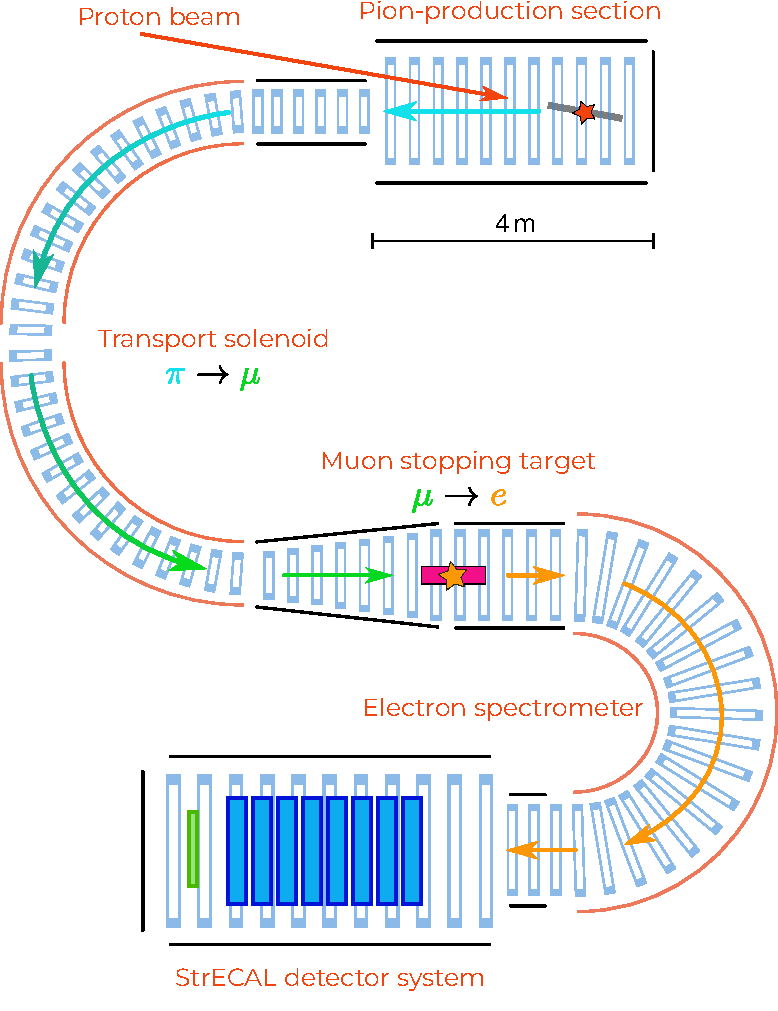
\includegraphics[width=\textwidth]{chapter2/comet_schematic.pdf}
        \caption{Phase-II.}
    \end{subfigure}
    \caption{ Schematic top-down view of the COMET experiment. The beam pipe is
    represented in gray, and the light red rectangles along the beamline
    represent the solenoids that generate the magnetic field. Curved solenoids
    additionally help to select charge and momentum, as discussed in
    Section~\ref{sec:curved_solenoids}.}
    \label{fig:comet_schematic}
\end{figure}



\section{Proton beam}\label{sec:COMET_beam}

Muons in the COMET experiment are produced from the decay of pions created in
proton collisions on a static solid target. The primary proton beam is provided
by the J-PARC facility. Protons are delivered with an energy of \SI{8}{\GeV},
which is picked to maximise the pion yield while minimising the production of
anti-protons, a potential background source.

The timeline of a COMET event is shown in Figure~\ref{fig:timing_distributions}.
The beam has a pulsed time profile: protons are grouped into \SI{100}{\ns}
bunches, each containing $16\times 10^6$ protons. Bunches are separated by
\SI{1170}{\ns}. Just after the collision, secondary particles will quickly move
down the COMET beamline and produce numerous background hits in the detector
system. This prompt and intense flooding of the detector is called the
\emph{beam flash}, and typically dies down within a few hundred nanoseconds.
Muons bound by the muon stopping target have a lifetime of \SI{864}{\ns} (see
Section~\ref{sec:stopping_target}). This, combined with the \SI{1170}{\ns} time
span between two bunches, allows COMET to search for $\mu$--$e$ conversion after
the beam flash has ended, and until the next collision occurs. 

\begin{figure}
    \centering
    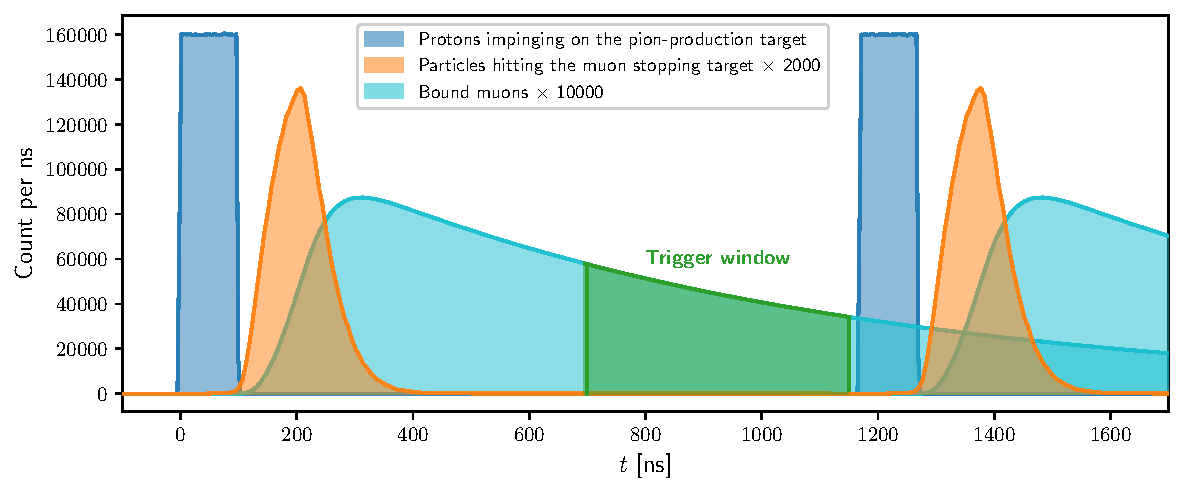
\includegraphics[width=0.85\textwidth]{chapter2/timing_plot_realistic_beam_flash.pdf}
    \caption{ Timeline of a COMET event. Shortly after the proton collision, the
        beam flash floods the detector and muons begin to be bound in the muon
        stopping target. The Phase-I trigger window shown here starts at
        $t=\SI{700}{\ns}$ and lasts until the next proton bunch collision.  }
    \label{fig:timing_distributions}
\end{figure}

% Could also add info on buckets, 4/5 time structure

Stray protons arriving in the time between two bunches can contribute to the
experimental backgrounds by sending particles toward the detector region at
unexpected timings. COMET requires the J-PARC proton beam to have fewer than one
such stray proton for every 600 bunches in order to reach its sensitivity goals.
This corresponds to an extinction factor
\begin{equation}\label{eq:extinction}
R_\mathrm{extinction} \equiv \frac{\mathrm{protons\ between\
bunches}}{\mathrm{protons\ per\ bunch}} \approx 10^{-10}.
\end{equation}

\section{Pion-production section}

\begin{figure}
    \centering
    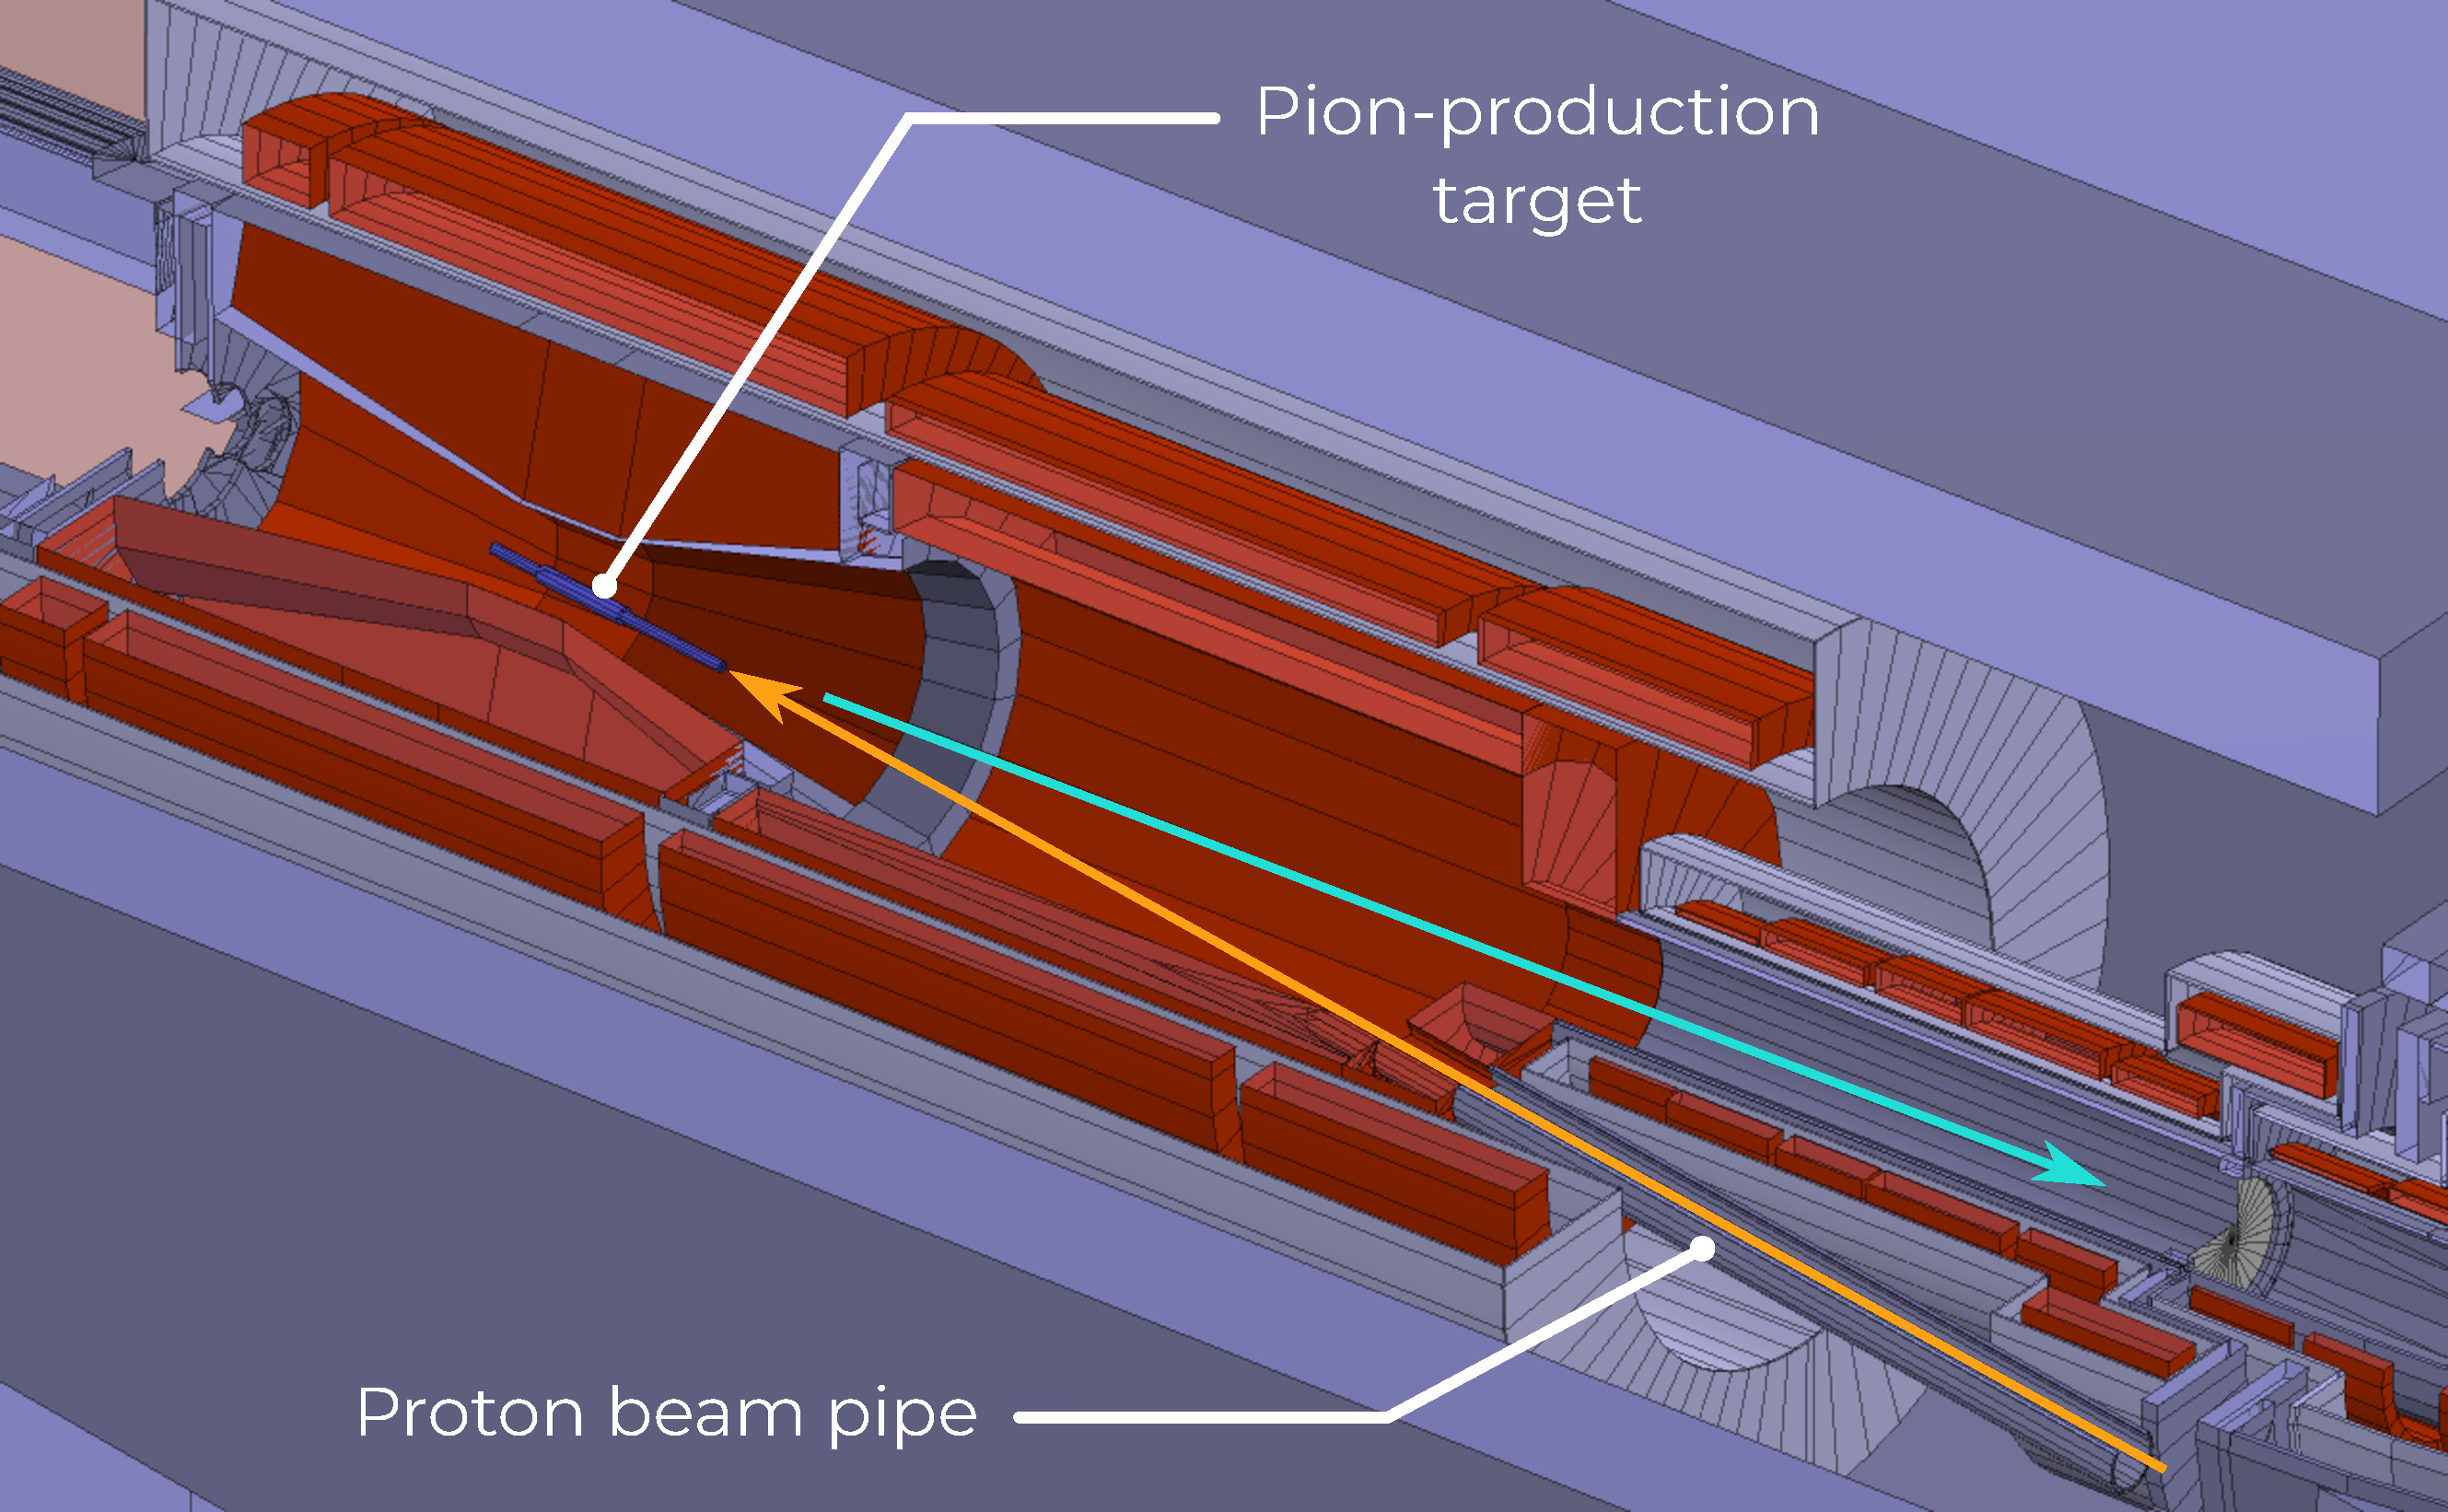
\includegraphics[width=0.8\textwidth]{chapter2/pion_production_section.png.pdf}
    \caption{ Cutaway view of the pion-production section. The orange arrow
        indicates the path of the proton beam while the teal arrow shows the
        direction of backward-going pions captured by the magnetic field.}
    \label{fig:pion_production_section}
\end{figure}

Pions are produced by the collision of the proton beam on a solid target made of
graphite in Phase-I, and tungsten in Phase-II. This region is permeated by a
\SI{5}{\tesla} magnetic field produced by a superconducting solenoid, which
confines the pions and directs them toward the transport solenoid.
Figure~\ref{fig:pion_production_section} shows a cutaway view of this
region.


Pions produced moving backward with respect to the proton beam have a lower
energy than those produced going forward, although they are not as numerous. In
COMET, it is crucial to eliminate high-energy particles in the muon beam that
could produce secondaries mimicking the conversion signal. Hence, the beamline
is positioned in the opposite direction to the proton beam such that only those
low-energy backward-moving pions are allowed into the COMET beamline.
Figure~\ref{fig:pion_momentum} illustrates this by showing that pions moving
backward with respect to the proton beam have a much lower momentum cut-off than
forward-moving pions.

\begin{figure}
    \centering
    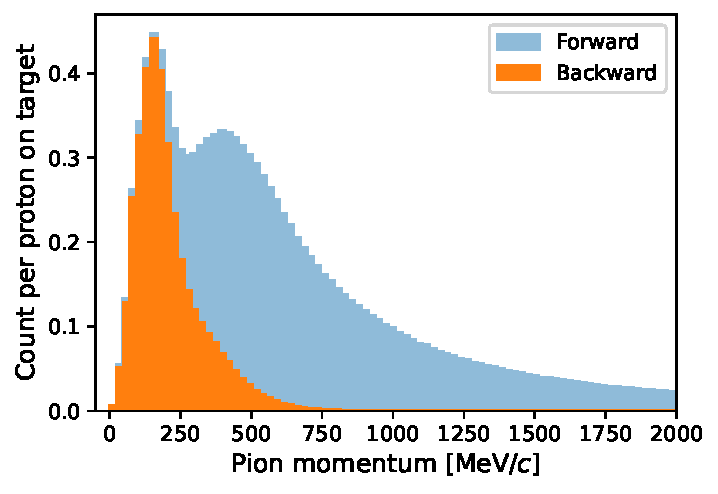
\includegraphics[width=0.5\textwidth]{chapter2/pion_mom-v2.pdf}
    \caption{ Momentum distribution of pions produced by simulating proton
    collisions with Geant4, depending on whether their initial direction is
    forward or backward with respect to the proton beam direction. }
    \label{fig:pion_momentum}
\end{figure}

\section{Transport solenoid}\label{sec:curved_solenoids}

\begin{figure}
    \centering
    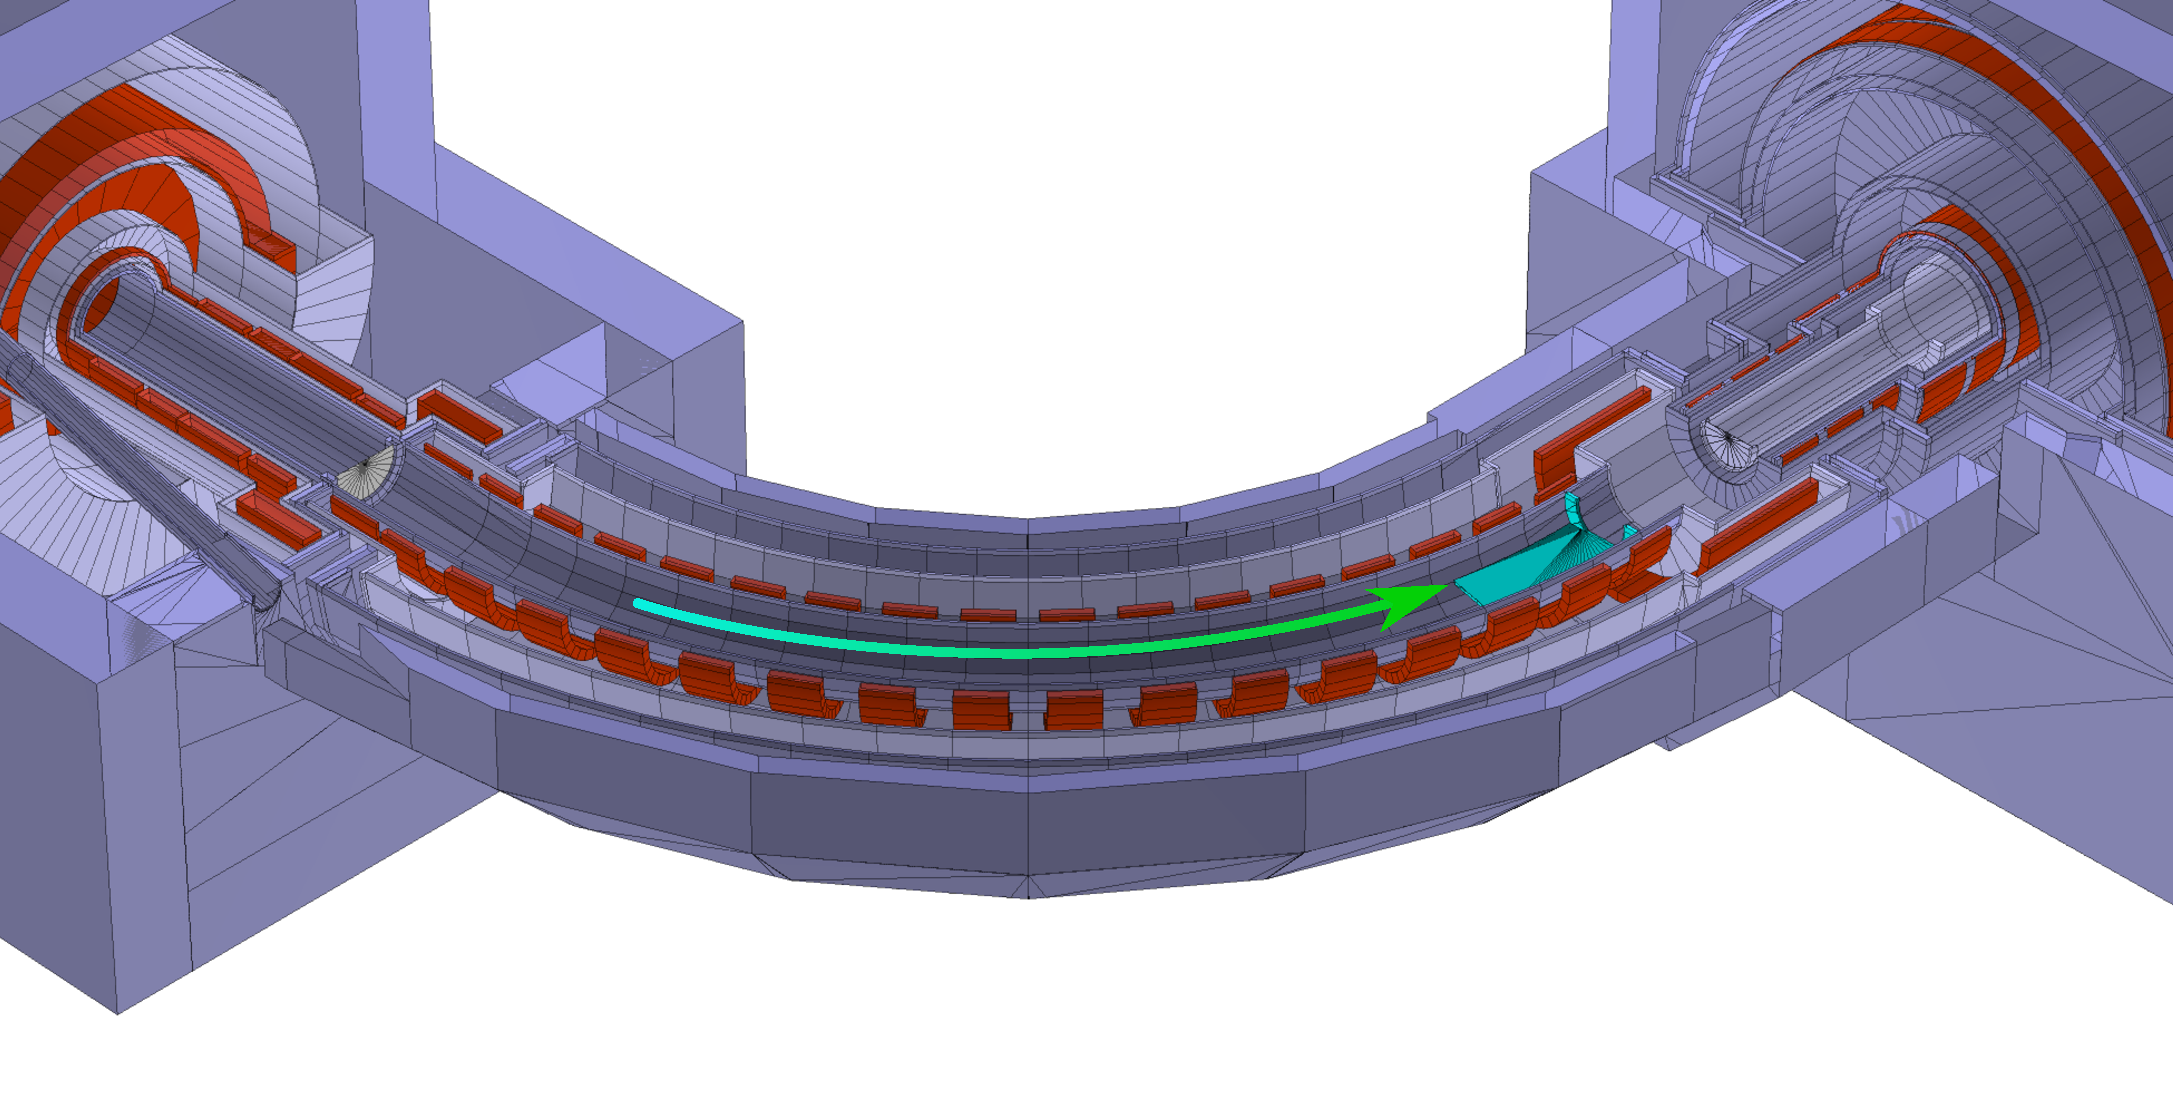
\includegraphics[width=0.8\textwidth]{chapter2/transport_solenoid.pdf}
    \caption{ Cutaway view of the Phase-I transport solenoid. The curved
        solenoid (in red) combined with collimators (in teal) select particles
        depending on their charge and momentum. }
    \label{fig:transport_solenoid}
\end{figure}

The transport solenoid is a curved pipe connecting the pion-production section
to the muon stopping section. Its purpose is twofold. Firstly, it allows a
larger fraction of pions to decay along the length of the beamline. Secondly,
the curved shape combined with its magnetic field and collimators allows it to
select negatively charged particles of a specific momentum. 


The magnetic field of a curved solenoid is slightly stronger on the inside of
the curve than on the outside. Since charged particles follow helical
trajectories, this has the net effect of making them drift vertically and the
amount of drift $D$ depends on momentum $p$ according to the equation
\begin{equation*}
    D = \frac{1}{q B} \frac{s}{R} \frac{2 p^2_L + p^2_T}{2 p_L},
\end{equation*}
where $q$ is the charge, $B$ is the strength of the field along the gyration
axis, $s$ is the distance travelled along the solenoid, $R$ is the radius of the
curve, and $p_L$ and $p_T$ respectively denote momentum longitudinal and
transverse to the solenoid axis~\cite{ben_thesis}. From this expression, one can
see that oppositely charged particles drift in opposite directions, and that
drift is overall stronger for higher-momentum particles. The ratio
$\frac{p_L}{p_T}$, which defines a helical trajectory's \emph{pitch angle}, is
also a major factor in a particle's drift.

\begin{figure}
    \centering
    \begin{subfigure}[b]{0.46\textwidth}
        \centering
        \hspace{-0.8cm}
        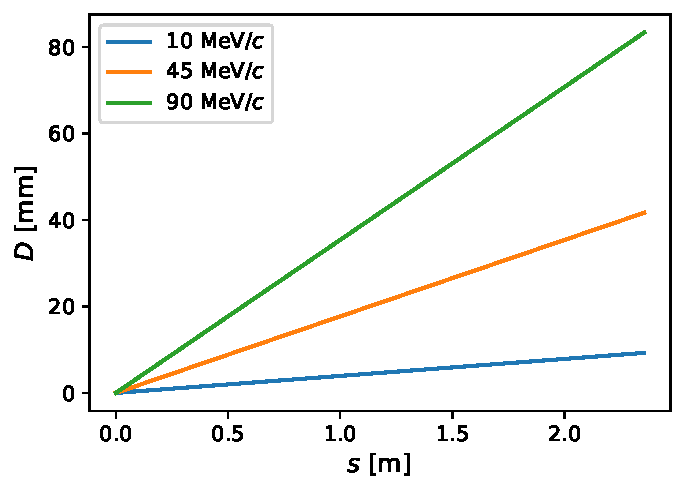
\includegraphics[width=\textwidth]{chapter2/drift_vs_s_0mT.pdf}
        \caption{No dipole field.}
    \end{subfigure}
    \hfill
    \begin{subfigure}[b]{0.46\textwidth}
        \centering
        \hspace{-0.8cm}
        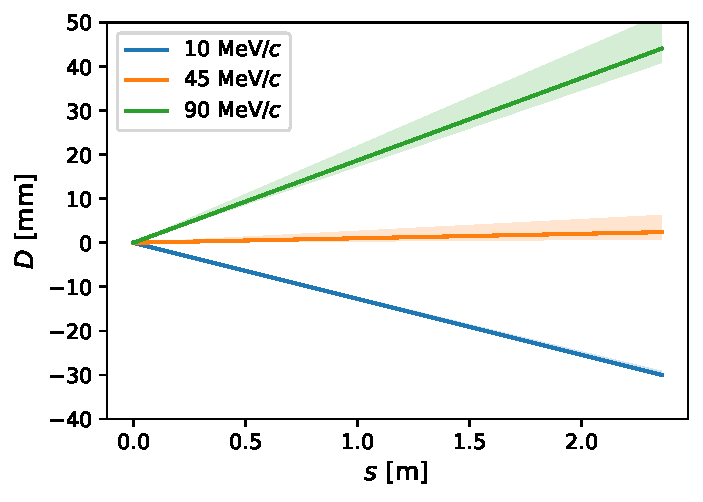
\includegraphics[width=\textwidth]{chapter2/drift_vs_s_0.05mT.pdf}
        \caption{\SI{0.05}{\tesla} vertical dipole field.}
    \end{subfigure}
    \caption{ Effective drift of particles of various momenta as they progress
        along the Phase-I transport solenoid. Solid lines show drift for a pitch
        angle of \SI{45}{\degree}, and the surrounding bands show the effect of
        a $\pm \SI{10}{\degree}$ change in pitch angle on the drift. By applying
        an additional vertical magnetic field, particles of a specific momentum
        can be selected. Here, a \SI{0.05}{\tesla} dipole field allows
        particles around \SI{45}{\MeV/\clight} to stay on axis while higher- and
        lower-momentum particles drift in opposite directions, and can then be
        suppressed by collimators at the end of the transport section. }
    \label{fig:drift}
\end{figure}

The drift caused by the curved solenoid makes all particles of the same charge
move in the same direction to varying degrees depending on momentum. In order to
select particles of a specific momentum, a vertical component is added to the
magnetic field to counterbalance the drift. Selected particles thus stay on
axis, while higher- and lower-momentum particles drift off axis. With the addition
of a collimator at the end of the transport solenoid, particles with unwanted
momenta are effectively eliminated from the beam.

Figure~\ref{fig:drift} shows drift $D$ as a function of $s$, the longitudinal
distance travelled by particles along the solenoid. This illustrates how, by
adding a dipole field, particles with a momentum outside the required range can
be efficiently eliminated by collimators at the top and bottom of the beam pipe.

\section{Muon stopping target}\label{sec:stopping_target}
The purpose of the muon stopping target is to slow down and stop as many muons
as possible while not blocking the path of converted electrons. It is composed
of a series of 17 thin aluminium disks placed in the way of the muon beam. The
disks are \SI{20}{\cm} in diameter, \SI{0.2}{\mm} thick, and separated by
\SI{5}{\cm}. The stopping target is shown in Figure~\ref{fig:cydet}, surrounded
by the Cylindrical Detector.

The more aluminium there is, the higher the number of muons that will be stopped
and allowed to undergo conversion. However, more material also means more energy
lost by electrons flying outward, hence the design of the target optimises
between muon stopping rate and acceptance of conversion electrons by the
detector system.


The material of the stopping target influences the conversion rate, but also the
lifetime of a muon caught in orbit around a nucleus. A heavy target favours the
expected rate of $\mu$--$e$ conversion, however it also causes the nuclear
capture rate to be higher. In COMET, beam bunches are separated by
\SI{1.17}{\ns} and prompt backgrounds typically die off within a few hundred
nanoseconds. A muonic atom with an iron or heavier nucleus has a lifetime less
than \SI{200}{\ns}~\cite{ben_thesis}, which would be too short to allow muons to
stay bound and convert after the beam flash is over. Hence, a light target such
as aluminium, with a longer stopped muon lifetime of
\SI{864}{\ns}~\cite{PhysRevC.35.2212}, is better suited to the COMET conversion
search.

\section{Detector systems}
\subsection{StrECAL}
The StrECAL combines a straw-tube tracking detector with an electromagnetic
calorimeter for energy measurement. In COMET Phase-I, the StrECAL will serve as
a beam characterisation apparatus. It will be placed directly at the end of the
transport solenoid, without a muon stopping target, to study the composition of
the COMET beam and gain a more thorough understanding of potential backgrounds.
The collected data can also serve to validate and refine the Monte Carlo
simulation in preparation for the conversion measurement.

In COMET Phase-II, the StrECAL will serve as the detector system for the
conversion measurement. It will be placed after the electron spectrometer, a
curved solenoid section designed to select conversion electrons, as shown in
Figure~\ref{fig:comet_schematic}. Figure~\ref{fig:strecal} shows a rendering of
the StrECAL detector system in Phase-II.

The Straw Tracker uses thin straw tubes as drift chambers, arranged into
circular planes. A series of stations, each one able to measure the horizontal
and vertical position of a particle, are positioned along the beam direction.
The straws have a resolution better than \SI{100}{\um}, which allows the Straw
Tracker to reconstruct trajectories and estimate particle momenta via
time-of-flight information.

The ECAL is a crystal electromagnetic calorimeter which supplements the Straw
Tracker in measuring energy and thus in identifying electrons. The ECAL uses
lutetium-yttrium oxyorthosilicate (LYSO) as its scintillating crystals and
avalanche photodiodes to collect the emitted photons.


\begin{figure}
    \centering
    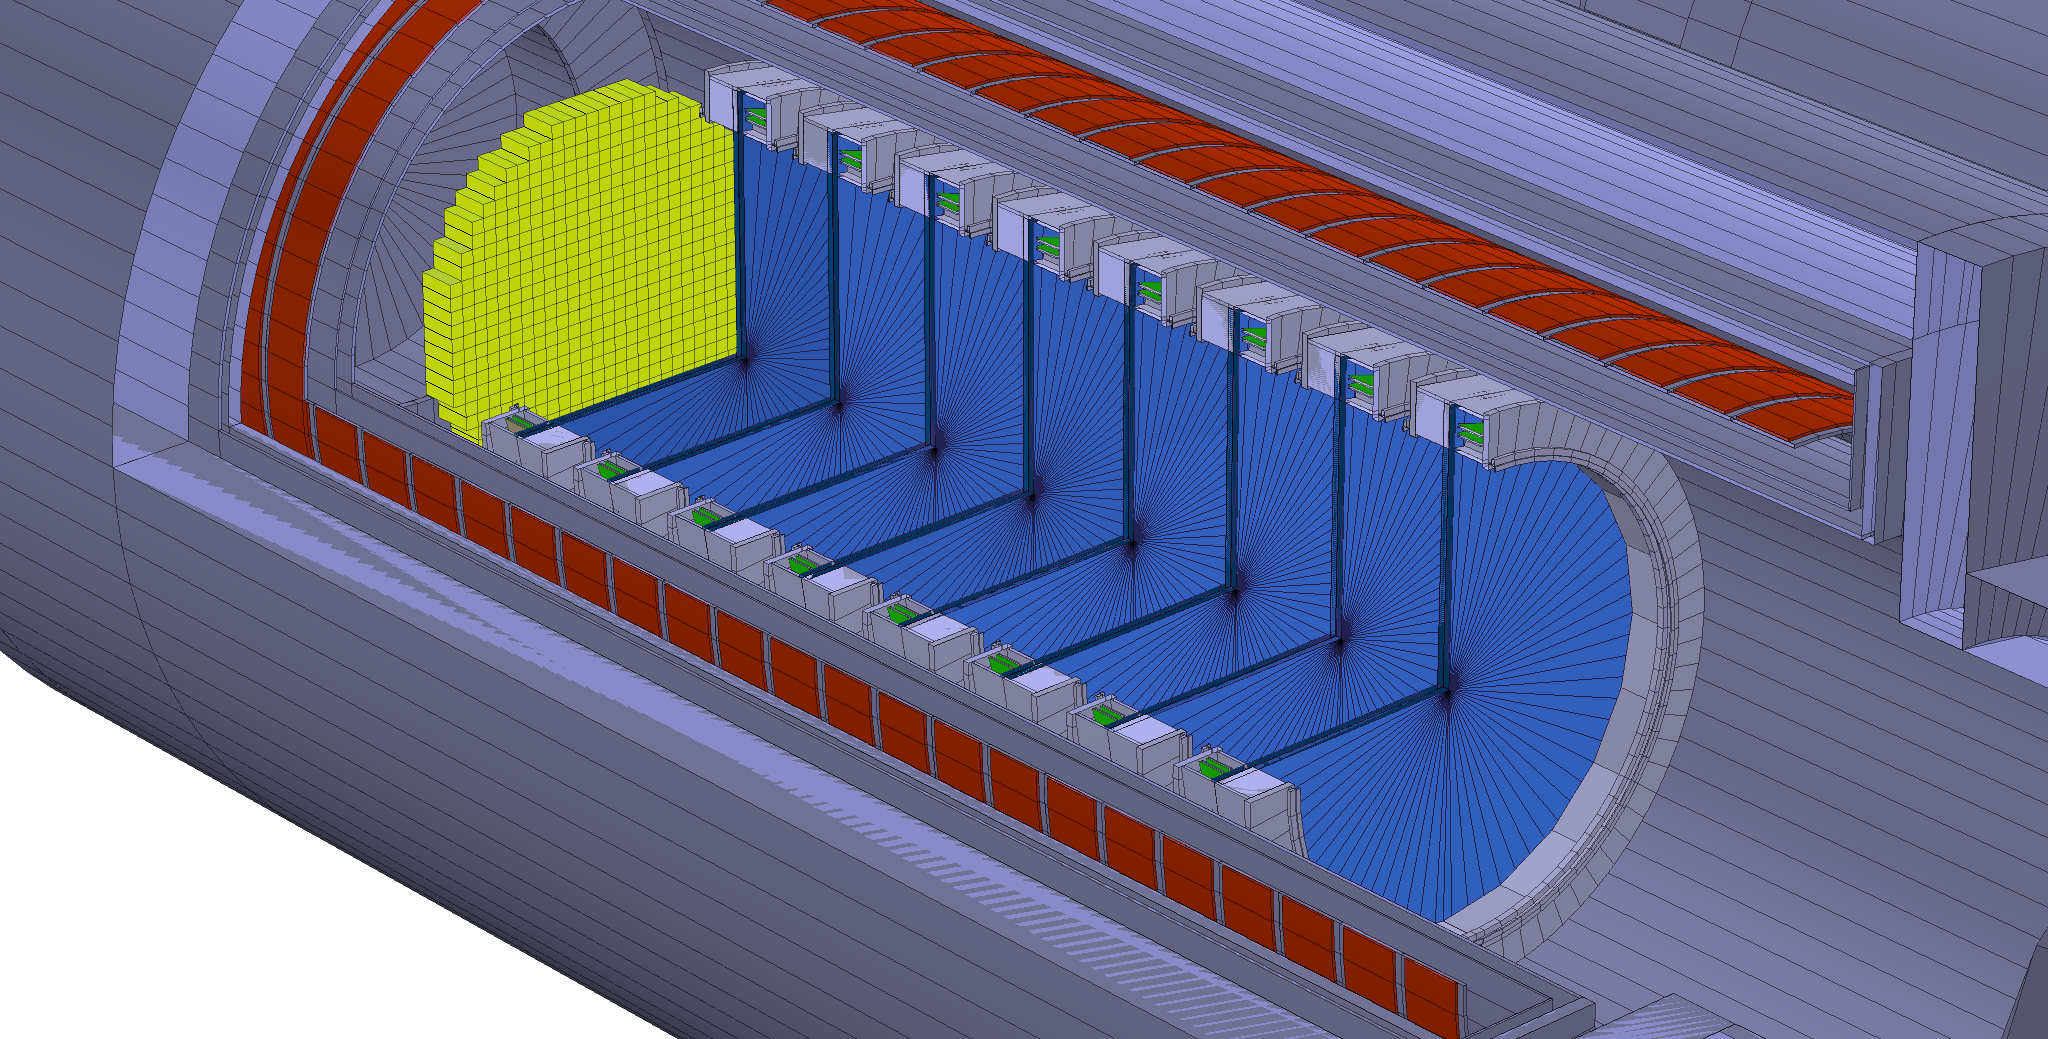
\includegraphics[width=0.8\textwidth]{chapter2/strecal_recolor.png}
    \caption{ Cutaway view of the StrECAL detector. The Straw Tracker stations
    are shown in blue and the ECAL in yellow.  }
    \label{fig:strecal}
\end{figure}

\subsection{CyDet}
The Cylindrical Detector (CyDet) consists of a Cylindrical Drift Chamber (CDC)
for tracking and a Cylindrical Trigger Hodoscope (CTH) for triggering on
specific event signatures. The CyDet surrounds the muon stopping target and sits
within the detector solenoid which generates a \SI{1}{\tesla} longitudinal
magnetic field. This configuration, shown in Figure~\ref{fig:cydet}, is designed
to eliminate backgrounds from the beam itself as well as low-momentum products
of the collision while maximising the acceptance of conversion electrons.
Figure~\ref{fig:cydet_signal_event} additionally shows the signature of a
simulated conversion electron inside the CyDet system.

\begin{figure}
    \centering
    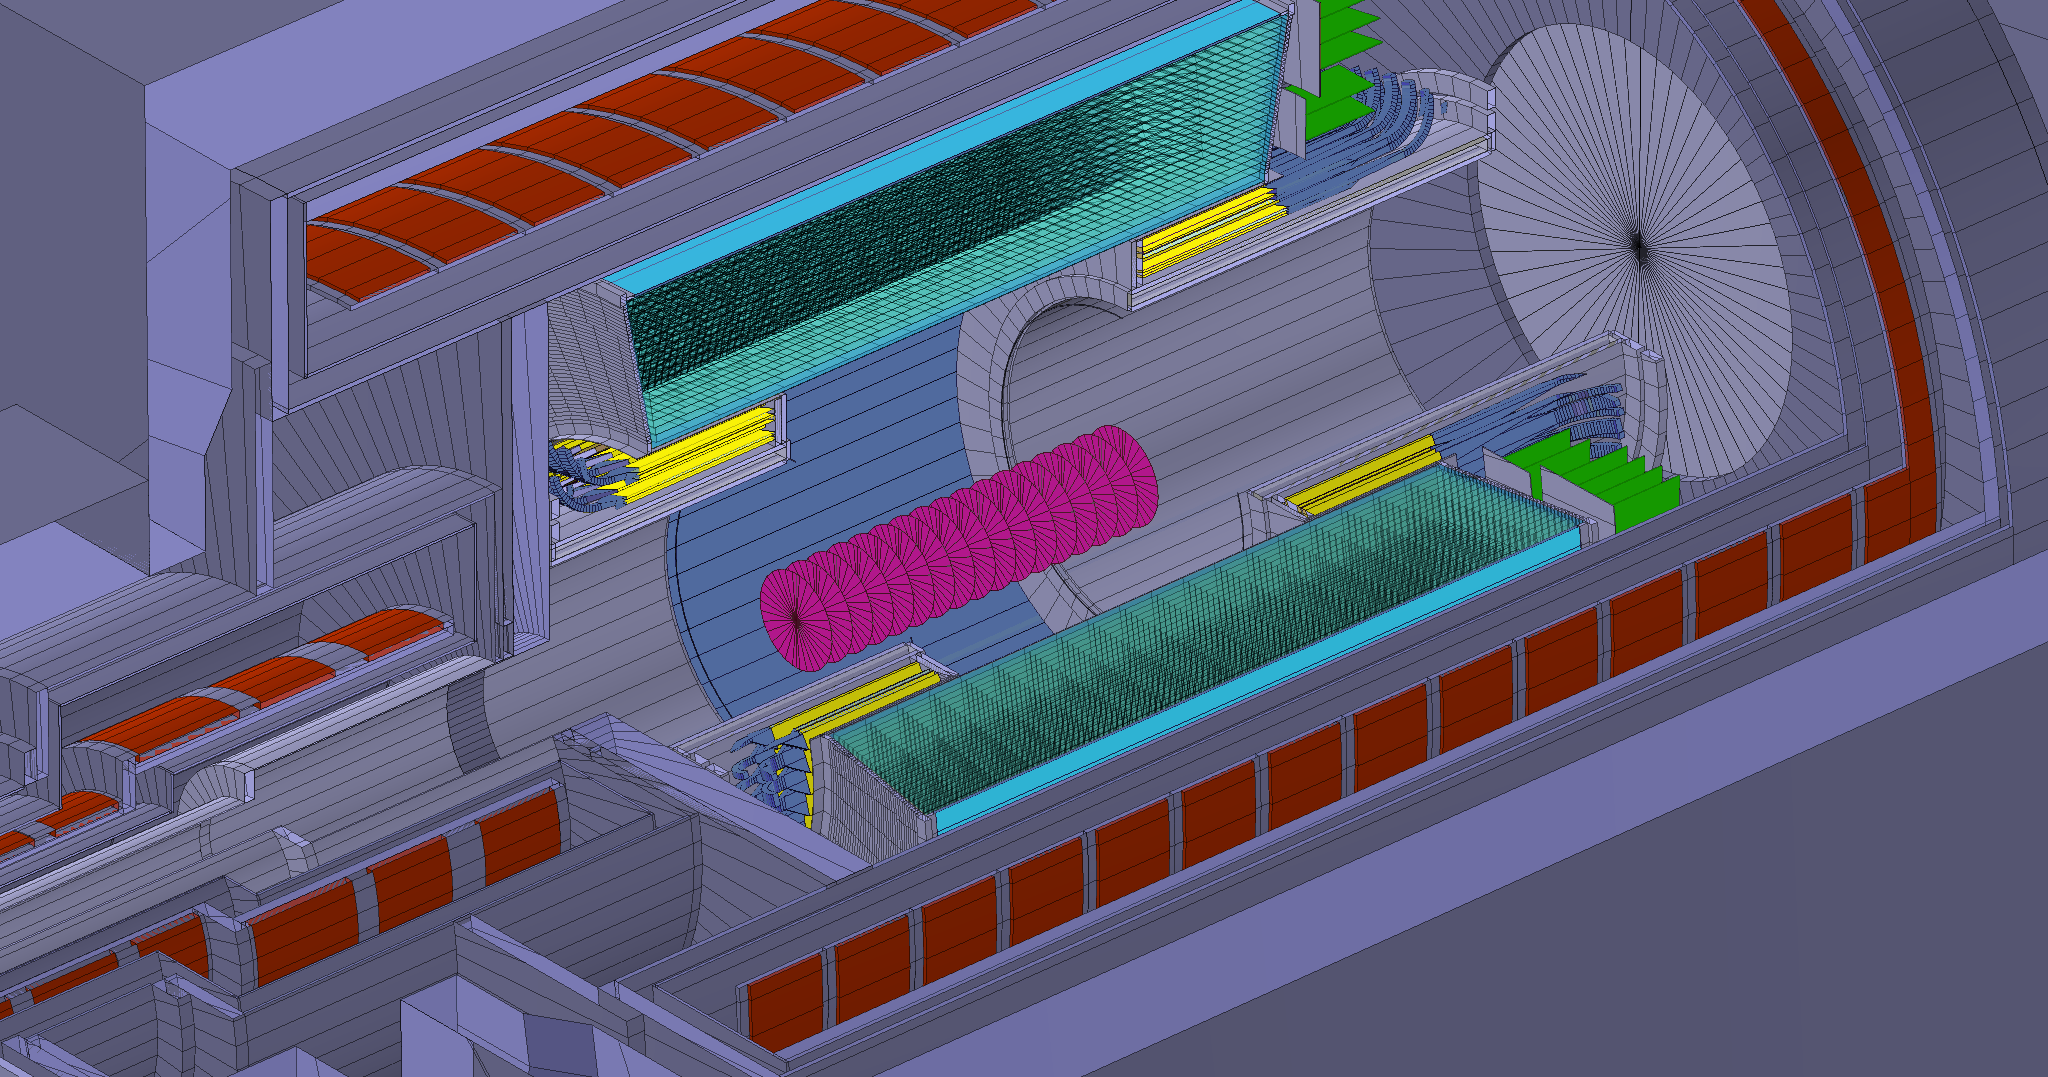
\includegraphics[width=0.8\textwidth]{chapter2/cydet_recolor.png}
    \caption{ Cutaway view of the Cylindrical Detector, composed of the
        Cylindrical Drift Chamber (in teal) and Cylindrical Trigger Hodoscope
        (in yellow). The muon stopping target disks, in purple, sit in the
        centre of the detector system. }
    \label{fig:cydet}
\end{figure}

\subsubsection{Cylindrical Drift Chamber}
The CDC is a drift chamber used to track charged particles emanating from the
muon stopping target. In order to suppress hits from beam particles, the CDC is
wrapped around the beam pipe and has an inner radius of \SI{50}{\cm}. Combined
with the \SI{1}{\tesla} longitudinal magnetic field, this prevents charged
particles with a transverse momentum less than \SI{60}{\MeV/\clight} from
reaching the chamber. In order to achieve the sensitivity goal for Phase-I, the
CDC has a momentum resolution better than \SI{200}{\keV/\clight} in order to
differentiate between conversion electrons and electrons from the high-energy
tails of the decay-in-orbit and radiative muon capture spectra. 

% Geometry
The CDC contains 4986 \emph{sense wires} strung out longitudinally in 20
concentric layers. The wires in each layer are rotated slightly off of the
longitudinal axis, and the rotation is alternatively clockwise and
anti-clockwise from one layer to the next. This special property, called the
\emph{stereo angle}, allows the drift chamber to stereoscopically reconstruct,
within \SI{3}{mm}, the longitudinal position of a particle~\cite{ewen_thesis}. 


% Operating principle
Each sense wire is held at a potential of up to \SI{1900}{\volt} and is
surrounded by 8 grounded \emph{field wires} to generate an inward electric
field. When a charged particle ionises the gas, the field accelerates freed
electrons toward the sense wire. These electrons can gain enough energy to further
ionise the gas, leading to avalanche multiplication (see
e.g.~\cite[Chapter~6]{leo}). The avalanche produces a pulse on the sense wire,
which is acquired by the readout electronics. 


% Drift time

% The time period between the passage of the ionising charged particle and the
% ionisation products inducing a pulse on the wire depends on the \emph{drift
% velocity} of the gas, which depends on the applied voltage.

% ... not necessary?

\subsubsection{Cylindrical Trigger Hodoscope}
The CTH consists of two \emph{modules} that line the inner wall of the CDC, one
upstream and one downstream of the muon stopping target. Each module contains
two layers of 48 partially-overlapping scintillation counters. Each counter has
a time resolution of \SI{1}{\ns}. The main purpose of the CTH is to reject
background events coming from the beam itself and from products of the muon beam
collision while complementing the CDC in identifying conversion electrons.

The overlap between counters allows the CTH to reject a large fraction of
background hits, e.g.\ from photons produced in the muon beam collision. This is
done by only accepting fourfold-coincident events, where four neighbouring
counters (two in the inner layer, two in the outer layer) are hit in a short
\SI{10}{\ns} time span. The CTH thus provides an online triggering mechanism
which significantly reduces the number of background events accepted by the
CyDet system due to its proximity with the muon stopping target.
Figure~\ref{fig:cydet_signal_event} shows how a conversion electron might
produce such a fourfold coincidence.


\subsection{Cosmic ray veto}\label{sec:crv}
The COMET experiment hall is constantly irradiated by muons produced in the
atmosphere by cosmic rays. The cosmic ray veto (CRV) is an additional active
detector which will tightly enclose the CyDet and StrECAL detector systems. Its
purpose is to identify events induced by cosmic muons rather than by the COMET
beam, and thus reduce the probability that such events will be mistaken for a
conversion signal.

\section{Conversion signature}
Conversion electrons are mono-energetic at $E=\SI{104.97}{\MeV}$ and emitted
isotropically by muons stopped in the target disks. In the magnetic field of the
detector solenoid, they have a helical trajectory which can be reconstructed by
the CDC or Straw Tracker. Figure~\ref{fig:cydet_signal_event} shows a simulated
conversion electron going through the Cylindrical Detector.



\begin{figure}
    \centering
    \captionsetup[subfigure]{justification=centering}
    \begin{subfigure}[b]{0.44\textwidth}
    \centering
    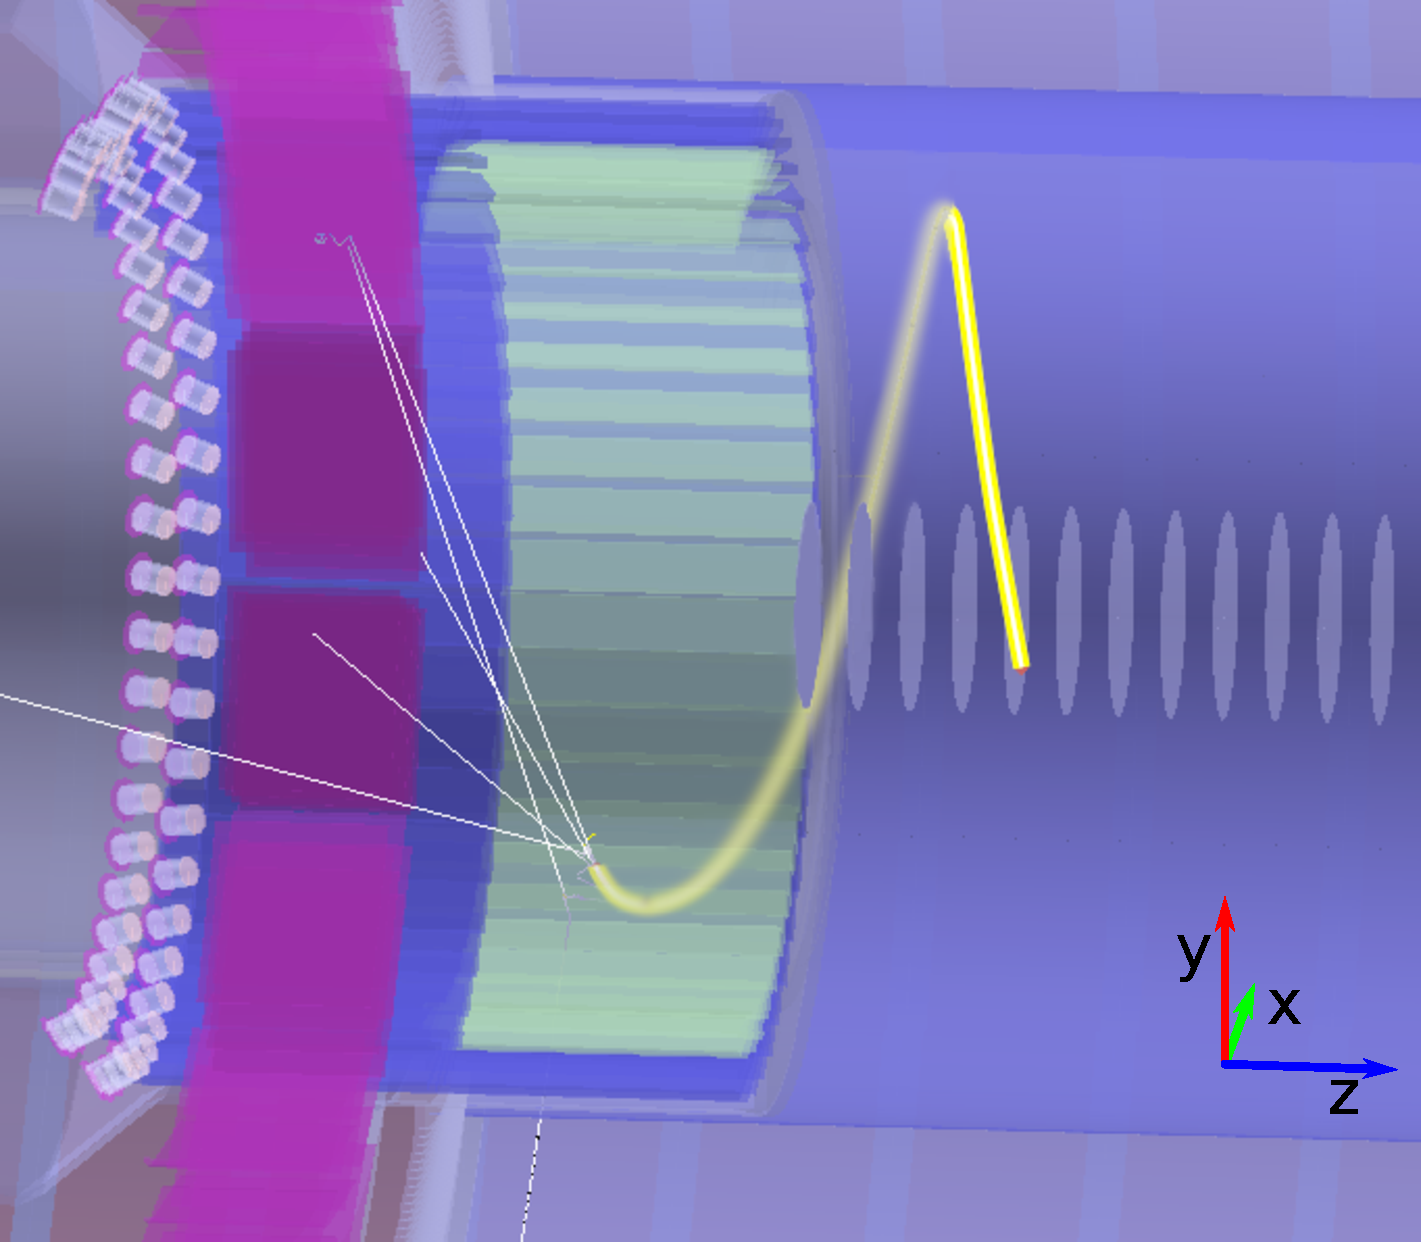
\includegraphics[width=0.85\textwidth]{chapter2/signal_event_display_crop_axes.pdf}
    \vspace{1.18cm}
    \caption{Event shown in \texttt{DisplayCore}, the 3D event display of
    ICEDUST (see Chapter~\ref{ch:software}).}
    \end{subfigure}
    \hfill
    \begin{subfigure}[b]{0.55\textwidth}
    \centering
    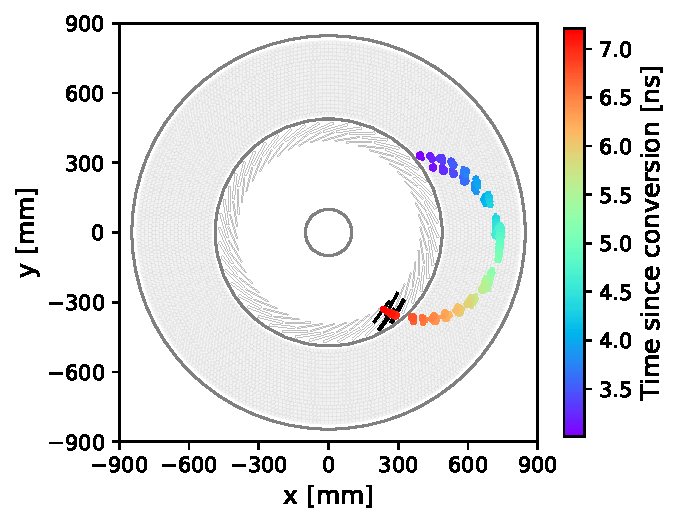
\includegraphics[width=0.99\textwidth]{chapter2/cydet_signal_track_v4.pdf}
    \caption{CyDet event display showing the timing of hits since conversion.}
    \end{subfigure}
    
    \caption{ Conversion electron trajectory as observed by the Cylindrical
    Detector. The effect of stereo angles is visible at the start of the
    trajectory where hits have alternating azimuthal positions around the actual
    electron track. Upon reaching the CTH, the electron produces consecutive
    hits in four adjacent counters, satisfying the fourfold coincidence trigger
    criterion.}
    \label{fig:cydet_signal_event}
\end{figure}


% Timing
The expected timing of conversion electrons is directly related to the time
distribution of muons bound inside the stopping target, shown in
Figure~\ref{fig:timing_distributions}. In Phase-I, in order to suppress prompt
backgrounds from the beam flash, the detector is tuned to only start triggering
on events that occur at least $t=\SI{700}{\ns}$ after each proton collision.
This acceptance criterion retains only \SI{30}{\percent} of all signal events
because the majority of bound muons, having an average lifetime of \SI{864}{\ns},
will have undergone decay or capture before the start of the window.


\section{Experimental backgrounds}\label{sec:backgrounds}

\begin{table}
    \centering
    \begin{tabular}{l|cccc|c}
        \toprule
        Background source & Intrinsic & Stray protons & Antiprotons &
        Cosmics  & Total\\ 
        Estimated events & 0.014 & 0.007 & 0.001 & 0.010 & 0.032 \\ \bottomrule
    \end{tabular}
    \caption{Expected number of background events from each potential
    source~\cite{the_comet_collaboration_comet_2020}. The total count is much
    smaller than one, such that the observation of a single signal electron
    could be evidence that charged lepton flavour is violated.}
    \label{tab:backgrounds}
\end{table}

Intrinsic backgrounds from muon decay-in-orbit and nuclear muon capture can
mimic the conversion signal, as discussed in Section~\ref{sec:sm_backgrounds}.
The COMET experiment is also affected by experimental backgrounds caused by the
intense beam, as well as cosmic ray-induced events.

Beam-induced backgrounds include delayed events caused by slow particles and
products of stray protons arriving between two bunches.
Antiprotons are the main source of delayed backgrounds due to their slow
speed relative to pions and muons of the same momentum. They are negatively
charged so cannot be efficiently selected out by the beamline, hence they can
collide late with the muon stopping target and produce signal-like secondary
electrons during the trigger window.

When a stray proton hits the pion-production target late, secondaries may
quickly travel to the detector region and produce a signal-like electron, which
can also be mistaken for the conversion signal. This is the main reason for
requiring the strict extinction factor $R_\mathrm{extinction}$ of
Equation~\ref{eq:extinction} from the J-PARC proton beam.

Finally, cosmic rays could be a major source of background events. The
background rate depends heavily on the amount of shielding and material above
the COMET detector system, as well as the efficiency of the cosmic ray veto. The
topic of rate estimation for cosmic ray-induced backgrounds is discussed more
thoroughly in Chapter~\ref{ch:cosmics}.



Table~\ref{tab:backgrounds} shows the rates estimated in the COMET Phase-I
technical design report (TDR)~\cite[Section
10.6]{the_comet_collaboration_comet_2020} for each source of background in the
$\mu$--$e$ conversion search. The total number of background events over the
data acquisition run time is predicted to be 0.032 given an extinction factor
$R_\mathrm{extinction} = 3 \times 10^{-11}$. Since this background event count
is much smaller than one, the observation of a single signal-like electron may
suggest that a CLFV process is at play, which would further motivate this search
through COMET Phase-II and beyond.



% Backgrounds = signal contamination. Backgrounds do not enter the equation for
% SES, but SES involves quality cut factors whose purpose is to lower background
% rates. The goal is to show that background rate << 1, only then SES makes
% sense since we've shown that we can actually detect a single event with little
% doubt that it's a conversion signal.


\section{Sensitivity and run time}\label{sec:SES}

The sensitivity of the COMET experiment is conventionally expressed as a
\emph{single event sensitivity} (SES), which is defined as the value of the
$\mu$--$e$ conversion branching ratio for which COMET expects to observe one
event (smaller is better). SES takes into account the net acceptance of signal events by the
detector system, however it does not say anything about the experimental
backgrounds. When using SES as a figure of merit, a study of potential
background sources is usually necessary to show that the expected number of
background events is not greater than one. 

The total number of coherent $\mu$--$e$ conversions produced by a
population of $N_\mu$ bound muons can be expressed as
$$
N_\mathrm{conversion} = N_\mu \cdot \mathcal{B}_\mathrm{conversion} \cdot
\mathcal{B}_\mathrm{capture} \cdot f_\mathrm{coherent},
$$
where $\mathcal{B}_\mathrm{conversion}$ is the conversion branching ratio
normalised to the branching ratio of nuclear muon capture
$\mathcal{B}_\mathrm{capture}$, and $f_\mathrm{coherent}$ is the fraction of
conversions estimated to occur coherently and leave the nucleus in its ground
state.
The number of conversion electrons that will be observed by the detector is then
$N_\mathrm{obs} = N_\mathrm{conversion}\, A_{\mu-e}$, where $A_{\mu-e}$ is the
detector's net signal acceptance. If we require $N_\mathrm{obs} = 1$ and
rearrange to find the corresponding value of $\mathcal{B}_\mathrm{conversion}$,
we obtain the single event sensitivity:
\begin{equation}\label{eq:ses}
\mathrm{SES} \, \equiv \, \mathcal{B}_\mathrm{conversion}^{N_\mathrm{obs}=1}
 = \, \frac{1}{N_\mu \  A_{\mu-e} \  
\mathcal{B}_\mathrm{capture} \  f_\mathrm{coherent}}.
\end{equation}
In COMET Phase-I, the signal acceptance can be broken down into seven efficiency
factors: geometrical acceptance, hardware (trigger and data acquisition), track finding,
track reconstruction quality cuts, momentum window and trigger time window.
Table~\ref{tab:acceptance} lists these factors as they were estimated in the
COMET Phase-I TDR~\cite[Section 10.1]{the_comet_collaboration_comet_2020}. 

\begin{table}
    \centering
    \begin{adjustbox}{max width=1.1\textwidth,center}
    \begin{tabular}{l|cccccc|c}
        \toprule
        Factor & Geometrical & Hardware & Track-finding & Cuts & Momentum
        & Timing & Net
        \\ 
        Efficiency & \SI{26}{\percent} & \SI{81}{\percent} &
        \SI{99}{\percent} & \SI{70}{\percent} & \SI{93}{\percent} &
        \SI{30}{\percent} & \SI{4.1}{\percent} \\
        \bottomrule
    \end{tabular}
    \end{adjustbox}
    \caption{ Efficiency factors used to determine the signal acceptance in the
    COMET Phase-I TDR~\cite{the_comet_collaboration_comet_2020}. The net
    acceptance is the product of all efficiency factors. ``Cuts'' refers to
    track quality cuts, used to reject events with irregular tracks that cannot
    be accurately fitted and reconstructed.}
    \label{tab:acceptance} 
\end{table}

From the net signal acceptance $A_{\mu-e} = \SI{4.1}{\percent}$, we can now
estimate the total data acquisition run time required to reach the sensitivity
goal of the experiment, $\mathrm{SES} = 3\times 10^{-15}$, using
Equation~\ref{eq:ses}. The required number of bound muons is thus $N_\mu = 1.5
\times 10^{16}$. This quantity can be related to the total run time $T$ via the
proton beam current $I_p = \SI{0.4}{\micro\ampere}$ and the yield of stopped
muons per collision $R_{\mu / p} = 4.7\times 10^{-4}$:
$$
N_\mu = T \cdot \frac{I_p}{e} \cdot R_{\mu / p}.
$$
This equation is rearranged for $T$ to yield $T = 146$~days of data acquisition
for a Phase-I SES of $3 \times 10^{-15}$.

\chapter{Software and Simulation}
\label{ch:software}

\newcommand{\SimG}{\texttt{SimG4}\xspace}
\newcommand{\oaEvent}{\texttt{oaEvent}\xspace}
\newcommand{\Geant}{{\sc Geant4}\xspace}

% \begin{markdown}
% ---

% + Introduce ICEDUST, the COMET software suite
%     + Describe whole, then individual parts
%     + oaEvent
 
% + Important part of the software is the set of simulation tools
%     + COMET geometries
%     + Physics, "physics list"?
%     + Show signal event display
%     + SDs, CDC hit representation
%     + RooTracker files
%     + Proton beam input?
%     + Hit merging and bunch simulation
%     + Large-scale production, MC5: Sampling world, example of results?
    
    
% + Version control
% + Continuous integration (+ CD, docker containers)
    
% + Mention miscellanous contributions:
%     + Beginner's tutorial (installation, simulation, analysis)
%     + Move from CMT to CMake and from ROOT5 to ROOT6
%     + Memory leaks and errors
%     + Backward MC: perhaps just ref chapter

% + Animated visualisation of CyDet activity

% ---
% \end{markdown}

Experiments in high energy physics are commonly accompanied by the development
of a set of software tools to help in manipulating and analysing experimental
data. Simulations are used extensively to optimise experimental designs and
prepare for the collection of real data while the physical instruments ---
detectors, magnets, readout electronics and data acquisition systems --- are
being manufactured and assembled.

\section{The ICEDUST Software Suite}
The COMET collaboration develops a suite of software packages named ICEDUST
(Integrated COMET Experimental Data User Software Toolkit) to satisfy the
offline data-processing requirements of the experiment. Originally forked in
2013 from the software written for T2K's near detector system ND280, ICEDUST
supports the needs of the COMET experiment with regard to simulation, on-disk
data format, calibration, reconstruction and analysis.
Figure~\ref{fig:icedust_schematic} shows the flow of real and simulated data
within the ICEDUST framework, and lists the names of the key packages for each
step.


\begin{figure}
    \centering
    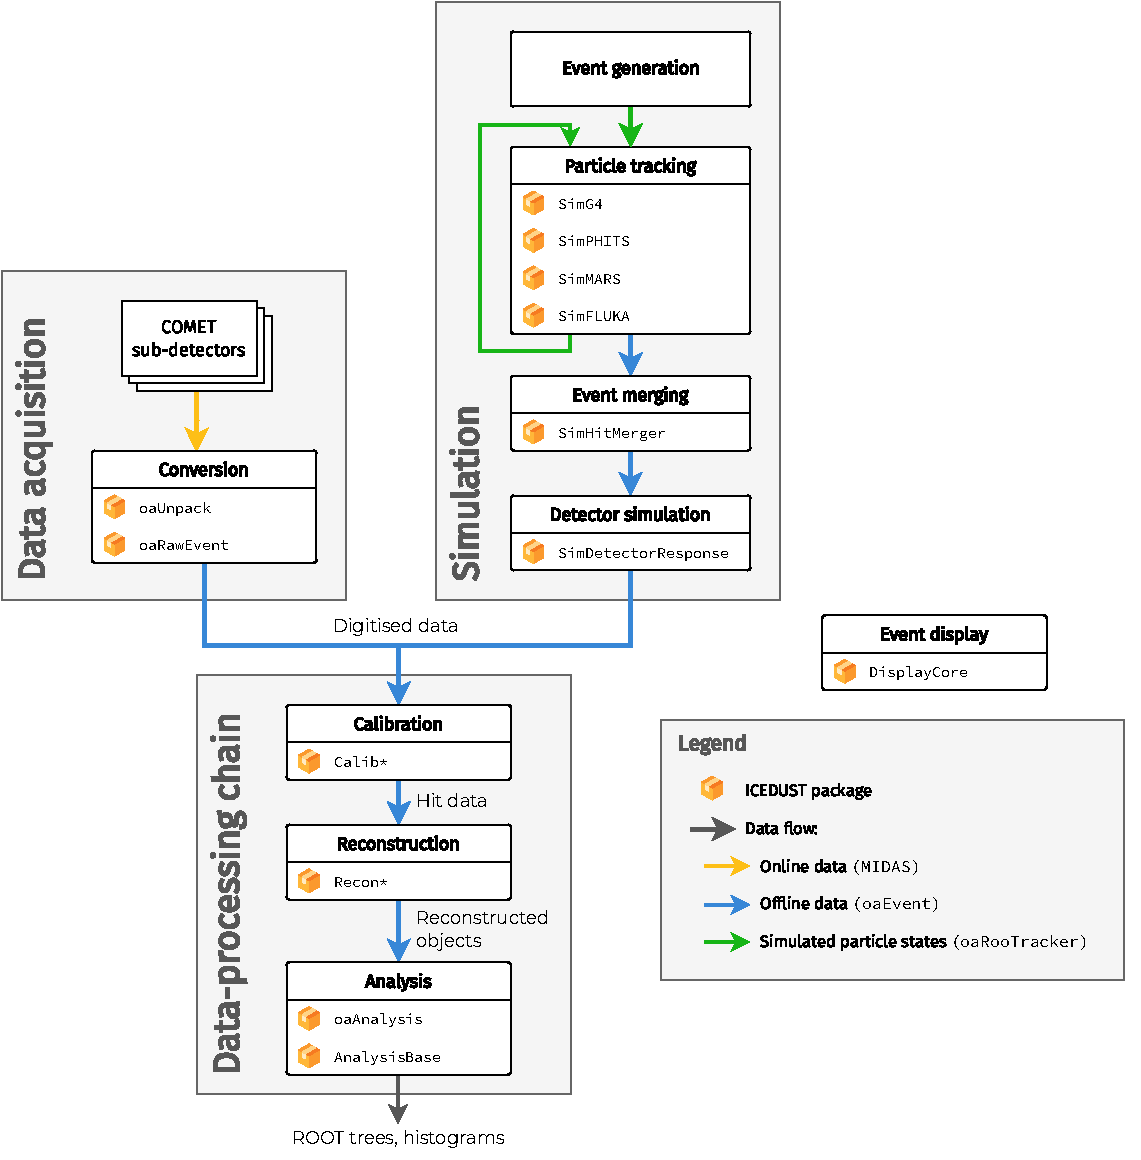
\includegraphics[width=0.9\textwidth]{chapter3/ICEDUST_vertical.drawio.pdf}
    \caption{Data flow in the ICEDUST framework. The colour of arrows represents
        the data format. By design, simulated detector data and real data share
        a common format such that they can be processed identically by the
        calibration, reconstruction and analysis stages.}
    \label{fig:icedust_schematic}
    \vspace{1.2cm}
    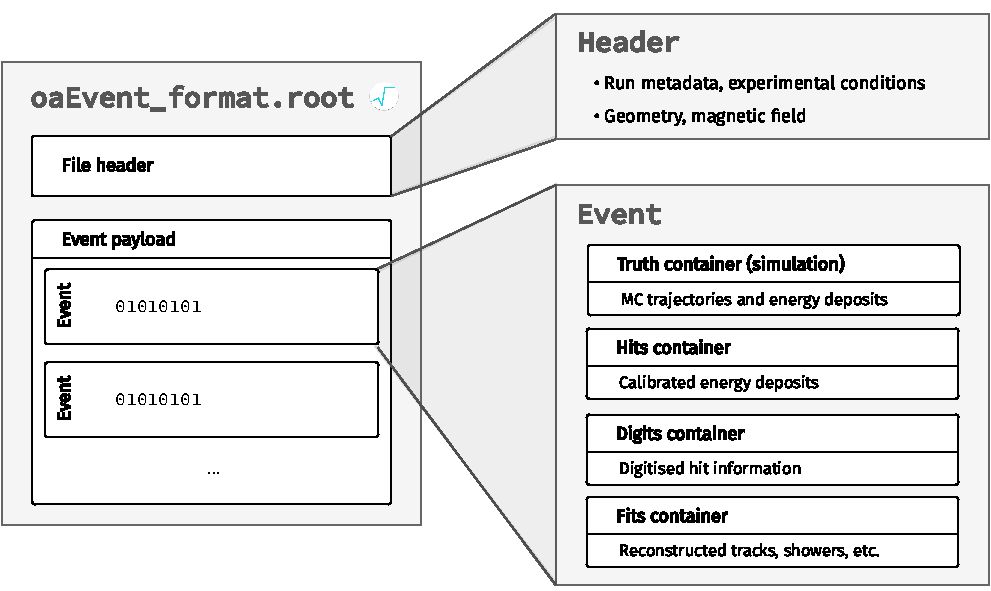
\includegraphics[width=0.6\textwidth]{chapter3/oaEvent.drawio.pdf}
    \caption{Layout of \oaEvent files which contain MC or real data. Blue arrows
    in Figure~\ref{fig:icedust_schematic} indicate steps of the data flow where
    data is stored in this format on disk.}
    \label{fig:oaEvent}
\end{figure}

\subsection{Data format}
A key design principle of ICEDUST is to define a common format adopted by both
real and simulated data, such that the pipeline of calibration, reconstruction
and analysis can be thoroughly tested with only simulation data, in advance of
the data acquisition stage. This offline data format is called \oaEvent. Based
on the ROOT~\cite{BRUN199781} serialisation system, \oaEvent defines a file
format where data is laid out as a sequence of events, shown schematically in
Figure~\ref{fig:oaEvent}. Each event object contains an arborescence of data
containers, each of which holds an array of some given data type (e.g.\ detector
hits, calibrated energy deposits, reconstructed tracks, etc.).

From Phase-I onward, data will be collected using the MIDAS data acquisition
system, hence the online on-disk format is based on MIDAS data banks. ICEDUST
provides a direct translation from this format to \oaEvent via the
\texttt{oaRawEvent} and \texttt{oaUnpack} packages. Once translated, the data
can flow through the calibration, reconstruction and analysis stages.

%Prior to calibration, the resulting data will typically represent uncalibrated,
%digitised detector hits or waveforms. 

%The term ``event'' here is purposefully abstract, as the information held in
%each event can vary. In simulations, an event can describe the outcome of a
%single proton-on-target (POT) collision, or the outcome of a full proton bunch
%($16\times10^6$ POT). 

%In data-taking runs, the definition of event will typically be dictated by the
%data acquisition system.  % So?



%Each event is its own hierarchical ``directory'', where data containers can be stored and retrieved by name. The containers themselves are variable-length arrays of arbitrary data types---defined as C++ classes---where objects of the same type can be aggregated.


%The calibration step uses pre-established calibration databases for each sub-detector to convert the digitised information into physical information such as the energy deposit and time that constitute hits. The reconstruction algorithms process hits to find tracks and filter out background, to pass that information down to the final analysis stage.

\subsection{Simulation pipeline}
Simulations of the COMET experiment can be split into four steps:
\begin{enumerate}
    \item {\bf Event generation} takes place at the level of individual protons.
    A proton beam profile is drawn ahead of time using a specialised
    Turtle~\cite{Carey1974DecayT} simulation of the beamline. The position and
    momentum of the protons are histogrammed at a short distance ahead of the
    pion-production target. Protons are sampled from the resulting distribution
    to generate events, and the outcome from each primary proton is referred to
    as a proton-on-target (POT) event.
    \item {\bf Particle tracking} is the step-by-step propagation of particles
    through the geometry and electromagnetic fields of the experimental setup.
    The primary proton will usually produce many secondary particles in the
    collision, some of which might propagate to the detector region. Simulated
    energy deposits in the active detector volumes are recorded for the detector
    response simulation stage.
    \item {\bf Event bunching} allows us to model the simultaneous arrival of a
    proton bunch into the setup. In the real beamline, millions of protons are
    bunched into a short \SI{{\sim} 100}{\ns} time interval, and two consecutive
    bunches are separated by about \SI{1.2}{\micro\second}. In order to simulate
    this time structure, a time offset is applied to each POT event, after which
    the events are merged into bunches. Following this, individual bunch events
    can be further merged into \emph{bunch trains} to obtain an entire sequence
    and account for potential pileup.
    \item {\bf Detector response simulation} translates the true energy deposits
    simulated in the particle tracking stage into detector-specific hits. It
    takes into account the way in which charge or light is collected by the
    detector, and can apply smearing to the observed energy and timing. This
    step effectively reverses the calibration process by transforming energy
    deposits into uncalibrated, digitised hits and waveforms.
\end{enumerate}

Once all four stages of the simulation pipeline are complete, the result should
closely resemble real data post-translation from MIDAS to \oaEvent. This implies
that it should be able to naturally flow through the calibration, reconstruction
and analysis stages. At each stage, the information may be compared with the
truth information available from the particle tracking stage in order to refine
each process. This exercise should also outline the performance of the offline
data-processing pipeline and hence provide an estimate of the computational
requirements of the experiment.


\subsection{Intermediate simulation file format}
\label{subsec:RT}
The \texttt{oaRooTracker} package defines another ROOT-based file format used by
the simulation to save and retrieve particle states. The typical use case is for
a simulation to record particles that have reached a key geometrical element
(e.g.\ the detector region) to build up a sample of interesting events. The
saved particle states can then be used as input to subsequent simulations,
easing the need for a full simulation run every time a change is made to the
geometry or physics models.

In addition, from a large enough sample of particles recorded at some key volume
boundary, the flux distribution of inbound particles can be estimated. Events
can then be sampled from this distribution to increase the statistics inside the
volume of interest. 

% RooTracker files
%The simulation software provides utility to record particles that reach certain
%key points in the geometry, such as the transport solenoid or the detector
%region. Virtual monitors are volumes that can be placed in the geometry to
%record the passage of particles, in the form of virtual hits or into a separate
%file. The file format used to save particle states is called
%\texttt{RooTracker}. It stores the kinematics of simulated particles and can
%thus be used as input to another simulation run. % and?

\section{Monte Carlo simulation in ICEDUST}
\label{sec:mc_sim}
Monte Carlo (MC) simulation is the process through which hypothetical particles
are realistically propagated through an experimental setup, with the aim of
evaluating the experiment's performance and to prepare for its realisation.
Currently, in COMET, MC simulations are heavily used to further optimise the
experiment's design and to develop reconstruction and analysis algorithms.

Monte Carlo simulation in high energy physics can be described as the stepwise
propagation (tracking) of particles through matter and electromagnetic fields.
Starting from initial conditions of position and momentum, a particle advances
in space and time according to the laws of relativistic kinematics. It can
change velocity or direction, and produce secondary particles via interactions
with the local medium and field. The tracking of a particle ends when it decays,
gets absorbed by some material, or exits the simulation space.

Interactions and decays occur stochastically according to measured
cross-sections and lifetimes. Depending on the type of interaction, secondary
particles may be emitted. In this case, the position and momentum of secondaries
are stored in memory until the tracking of the primary particle is finished. The
list of secondaries is then iterated through, propagating each one in turn.
Since secondaries may produce their own secondaries, this process continues
recursively until all products of the original primary particle have been
accounted for.

In ICEDUST, particle tracking, event bunching and detector response simulation
are handled in separate packages. Particle tracking can be performed using four
different engines: Geant4~\cite{AGOSTINELLI2003250}, FLUKA~\cite{FLUKA},
MARS15~\cite{MARS15} and PHITS~\cite{PHITS}. The corresponding ICEDUST packages
are \SimG, \texttt{SimFLUKA}, \texttt{SimMARS}, and \texttt{SimPHITS},
respectively. Event bunching is handled by the \texttt{SimHitMerger} package,
and \texttt{SimDetectorResponse} performs detector response simulation.

\subsection{Geometry}

\begin{figure}
    \centering
    %\captionsetup[subfigure]{justification=centering}
    % To make this figure: thin wireframes, white background
    % Plane clipping at y=10
    % zoom all the way out and move the camera forward (right-click)
    % so the perspective approaches an isometric view.
    \noindent\makebox[\linewidth][c]{
    \begin{subfigure}[t]{0.57\textwidth}
        \centering
        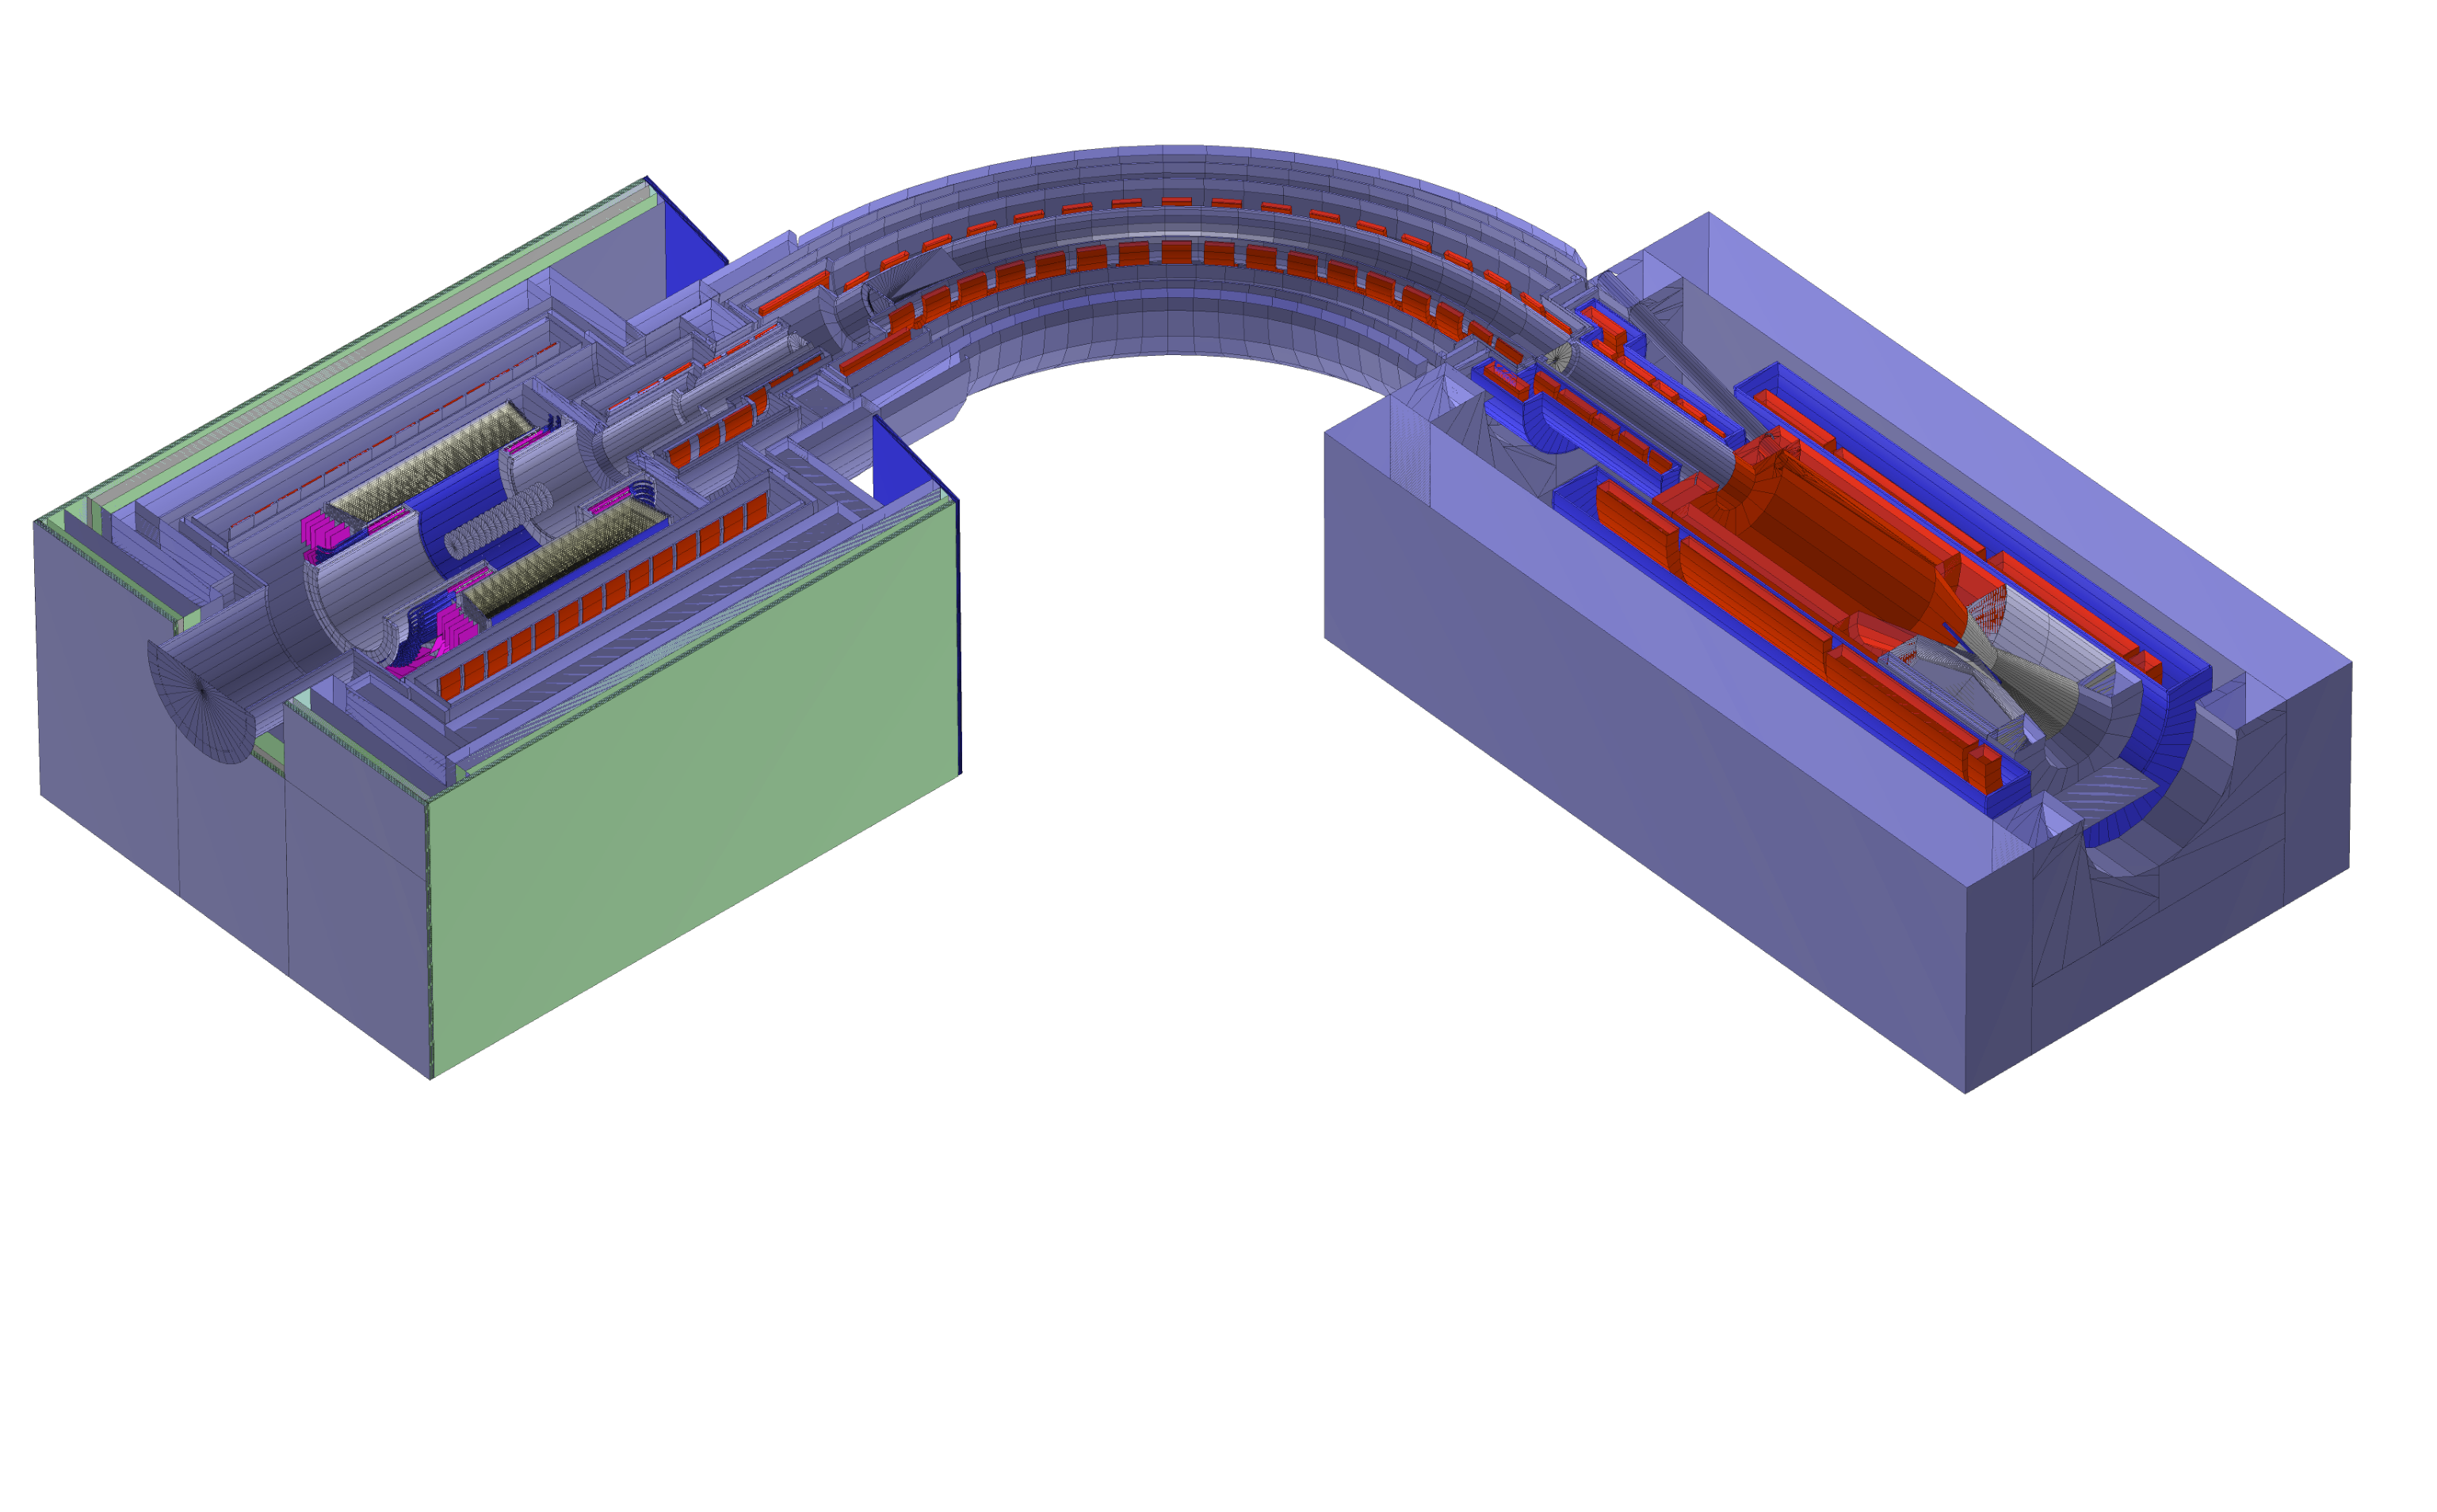
\includegraphics[width=0.95\textwidth]{
            chapter3/geometries_Phase-I_iso_cropless_huesat_croppedleft.png}
        \caption{Phase-I in the CyDet configuration.}
    \end{subfigure}
    \hfill
    \begin{subfigure}[t]{0.57\textwidth}
        \centering
        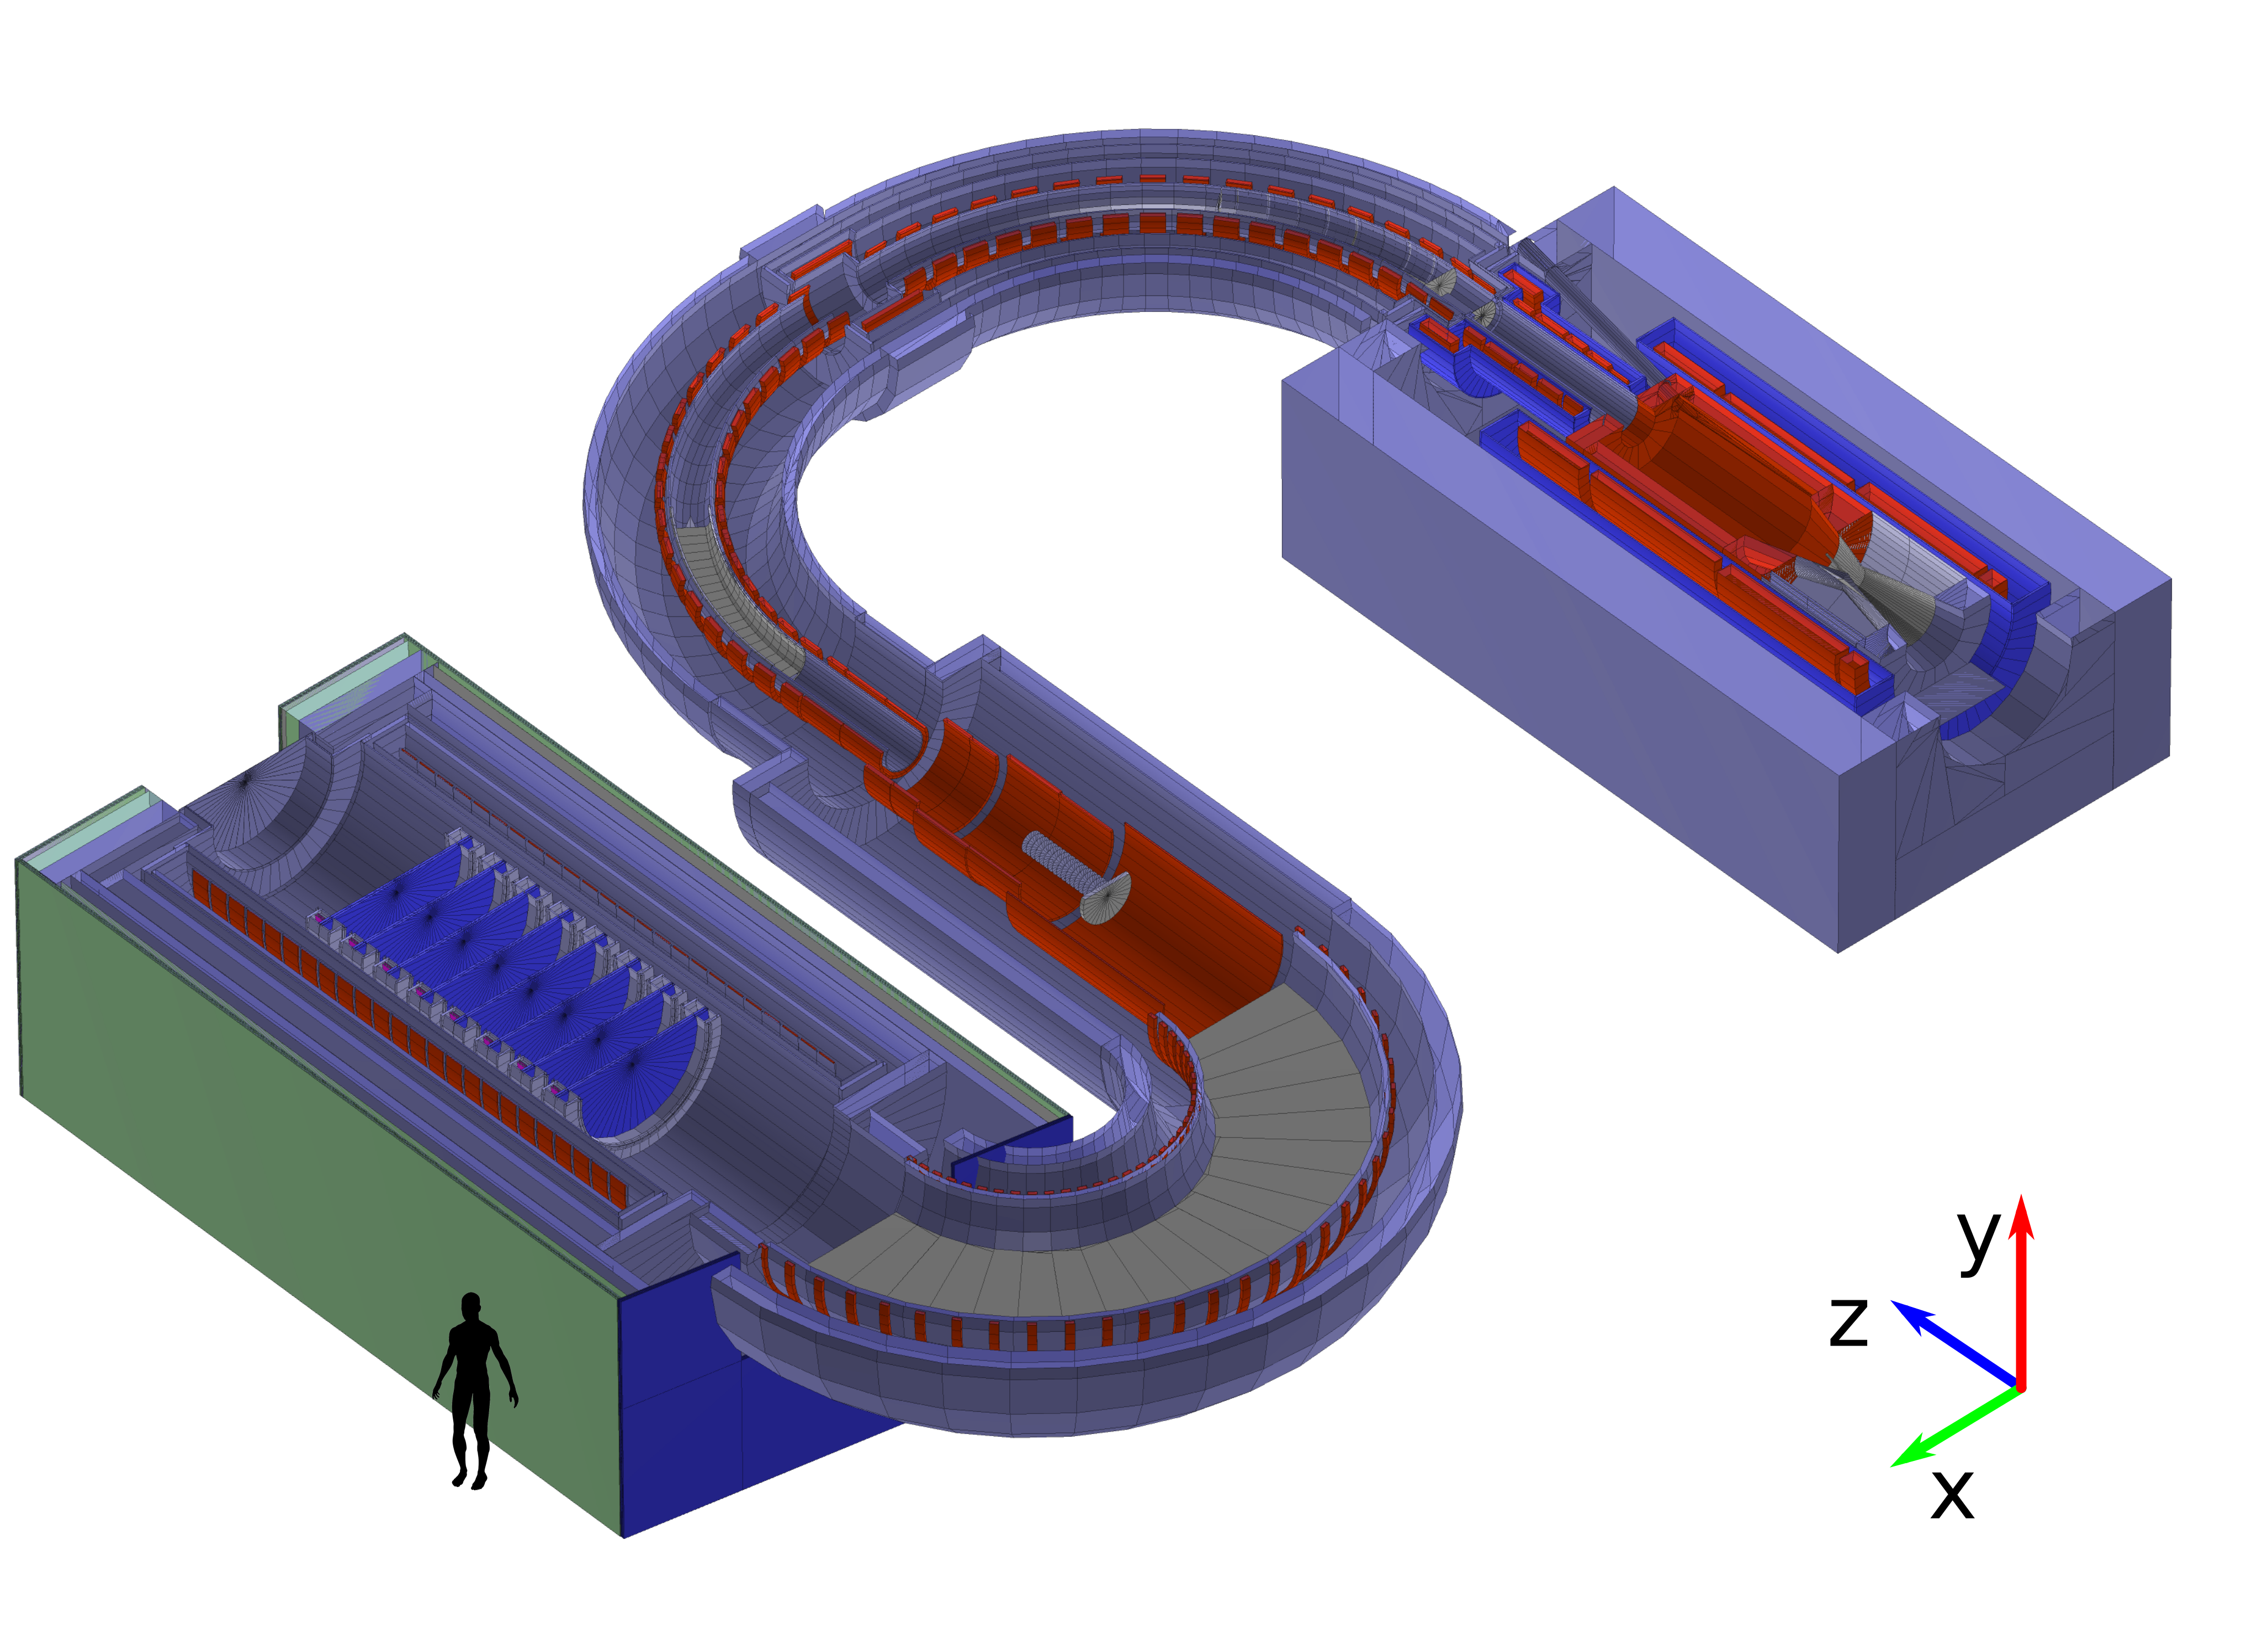
\includegraphics[width=0.95\textwidth]{
            chapter3/geometries_Phase-II_iso_huesat_human.png}
        \caption{Phase-II.}
    \end{subfigure}}
    
    \caption{Cutaway views of the simulation geometries implemented in \SimG and
    visualised with \texttt{DisplayCore}. The experiment hall is also modelled
    in the simulation but was hidden here for clarity.}
    \label{fig:comet_geometries}
\end{figure}

The \SimG package contains the most detailed and up-to-date definitions of the
COMET simulation geometries. The various components that make up a simulation
world are defined with constructive solid geometry, using the standard \Geant
geometry classes. In addition, \SimG extends the \Geant macro language to allow
geometrical parameters to be defined in macro files. The position, dimensions,
and material of every volume can thus be specified at run-time rather than
compile-time. A custom parser attached to every volume allows interdependencies
between components and supports looping, for instance to position identical
elements in a regular pattern.

Once the simulation geometry is assembled, it is also translated into the ROOT
\texttt{TGeo} representation, which simplifies its visualisation and its storage
on disk as metadata inside \oaEvent files. This representation can furthermore
be interpreted by the MARS15 tracking software, which simplifies the process of
running comparative simulations.


The \SimG package includes geometries for the Phase-I (CyDet and StrECAL
configurations) and Phase-II setups. Over time, these simulation worlds are
refined by developers to better reflect the exact configuration of the
experiment. Figure~\ref{fig:comet_geometries} shows the simulation geometries
for the two conversion-searching COMET designs.


% vvvv Moved to first section
% % Event generation 
% \section{Event generation and bunch structure}
% Protons are sampled from a beam profile histogram at a distance of
% \SI{70}{\cm} upstream of the target. The histogram is generated via a
% Turtle~\cite{Carey1974DecayT} simulation of the proton beamline.

% In the simulation, a single proton is sampled from the beam histogram for each
% event, which differs from the real situation in that the actual beam is
% arranged into bunches, each containing about 16 million protons. Hence we
% assume that proton collisions in a bunch are independent of each other, and we
% merge POT events into bunch events by overlaying the produced trajectories and
% hits. This task is handled by the \texttt{SimHitMerger} program after \SimG
% has finished simulating single-proton events. The time structure of the proton
% bunch is modelled as a square wave with a width of \SI{100}{\ns}. To simulate
% this structure, a time shift is sampled uniformly between -50 and \SI{50}{\ns}
% for each POT event and applied to every trajectory and hit.

% ----------

\subsection{Physics}
The COMET experiment involves many physical processes to go from the initial
proton collision to backgrounds in the detector. The MC simulation must
faithfully account for any process which could lead to backgrounds if we are to
realistically estimate the experiment's performance. Hence, the \SimG simulation
associates standard \Geant hadronic and electromagnetic physics lists with
custom logic for nuclear muon capture and muon decay-in-orbit.

To model hadronic interactions, \SimG uses the \texttt{QGSP\_BERT\_HP} reference
physics list as the default. In this model, hadron-nucleus interactions between
the \SI{8}{\GeV} proton beam and the pion-production target are handled by the
Bertini Cascade model~\cite{WRIGHT2015175}.

Muons at rest receive special treatment in \SimG due to their important
contribution toward the background rate. The default energy spectrum of
electrons from muon decay-in-orbit is replaced by the numerical evaluation
of~\cite{czarnecki}, which includes the effect of nuclear recoil and thus allows
electron energies up to \SI{104.973}{\MeV}. In addition, the nuclear muon
capture (NMC) model is replaced to adhere to the results of the AlCap
experiment~\cite{PhysRevC.105.035501} which measured the energy spectrum of
protons emitted after NMC in aluminium.




\subsection{Signal simulation}
By default, the list of physical processes considered by \SimG includes only
SM-allowed interactions and decays, and hence does not include $\mu$--$e$
conversion. In order to simulate signal events, one can manually produce
conversion electrons out of the muons stopped inside the stopping target.

From the normal beam simulation, one can estimate the spatial and temporal
distributions of muons being stopped in the stopping target, and subsequently
sample conversion electrons from them. In sensitivity studies, signal events are
commonly overlaid onto a pure background sample in order to evaluate the signal
acceptance and background rejection efficiencies of the hit filtering and track
finding routines.


Figure~\ref{fig:cydet_signal_event} shows a simulated conversion electron
emerging from the stopping target, depositing energy inside the CDC gas, to
eventually trigger the CTH by hitting four adjacent counters. 

\subsection{Representation of simulated CDC hits}
\label{subsec:SD}
% Sensitive detectors, truth-hit representation
As a particle passes through a material, it tends to lose energy to the medium,
e.g. through inelastic scattering or ionisation. In MC simulations, simulated
energy deposits must be recorded inside active detector elements in order for us
to determine the response of the detector and readout systems to the passage of
the particle.

Detector elements in a \Geant simulation are defined as ``sensitive volumes'',
and energy deposits of incoming particles are accumulated and recorded as
``hits''. The way in which hits are instantiated is typically dependent on the
type of detector, because of differing granularities between e.g.\ a plastic
scintillator and a drift chamber. A higher-granularity detector type requires
finer-detailed information, hence more hit instances along the trajectory.

In \SimG, the data type associated with CDC hits is called \texttt{IG4HitGas}.
When \Geant reports an energy deposit inside the CDC, an instance of that class
is created. If a particle makes multiple steps in a CDC cell, the deposit from
each step is accumulated into the same hit instance, such that only one instance
per particle per cell may exist. If a particle enters the same cell multiple
times, one hit instance is created per entry. This is shown in
Figure~\ref{fig:sim_cdc_hits}, where the position and granularity of
\texttt{IG4HitGas} instances is drawn along an electron's trajectory in the CDC.


% In early 2019, ICEDUST developers agreed to change the definition of hits
% inside the CDC gas volume in order to more accurately portray the energy
% deposit information in that detector. Along that process, I came to be
% thoroughly involved in the testing and refinement of this new CDC hit
% representation, named \texttt{IG4HitGas}. 

% A hit representation is formulated as a C++ class which holds the hit's data.
% It must be coupled to a sensitive detector class, whose role is to receive
% information from \Geant's particle tracking system and accumulate it into
% instances of the hit class. For example, the sensitive detector class for a
% calorimeter might produce hits containing the total energy deposited for each
% inbound particle as well as a timestamp.

\begin{figure}
    \centering
    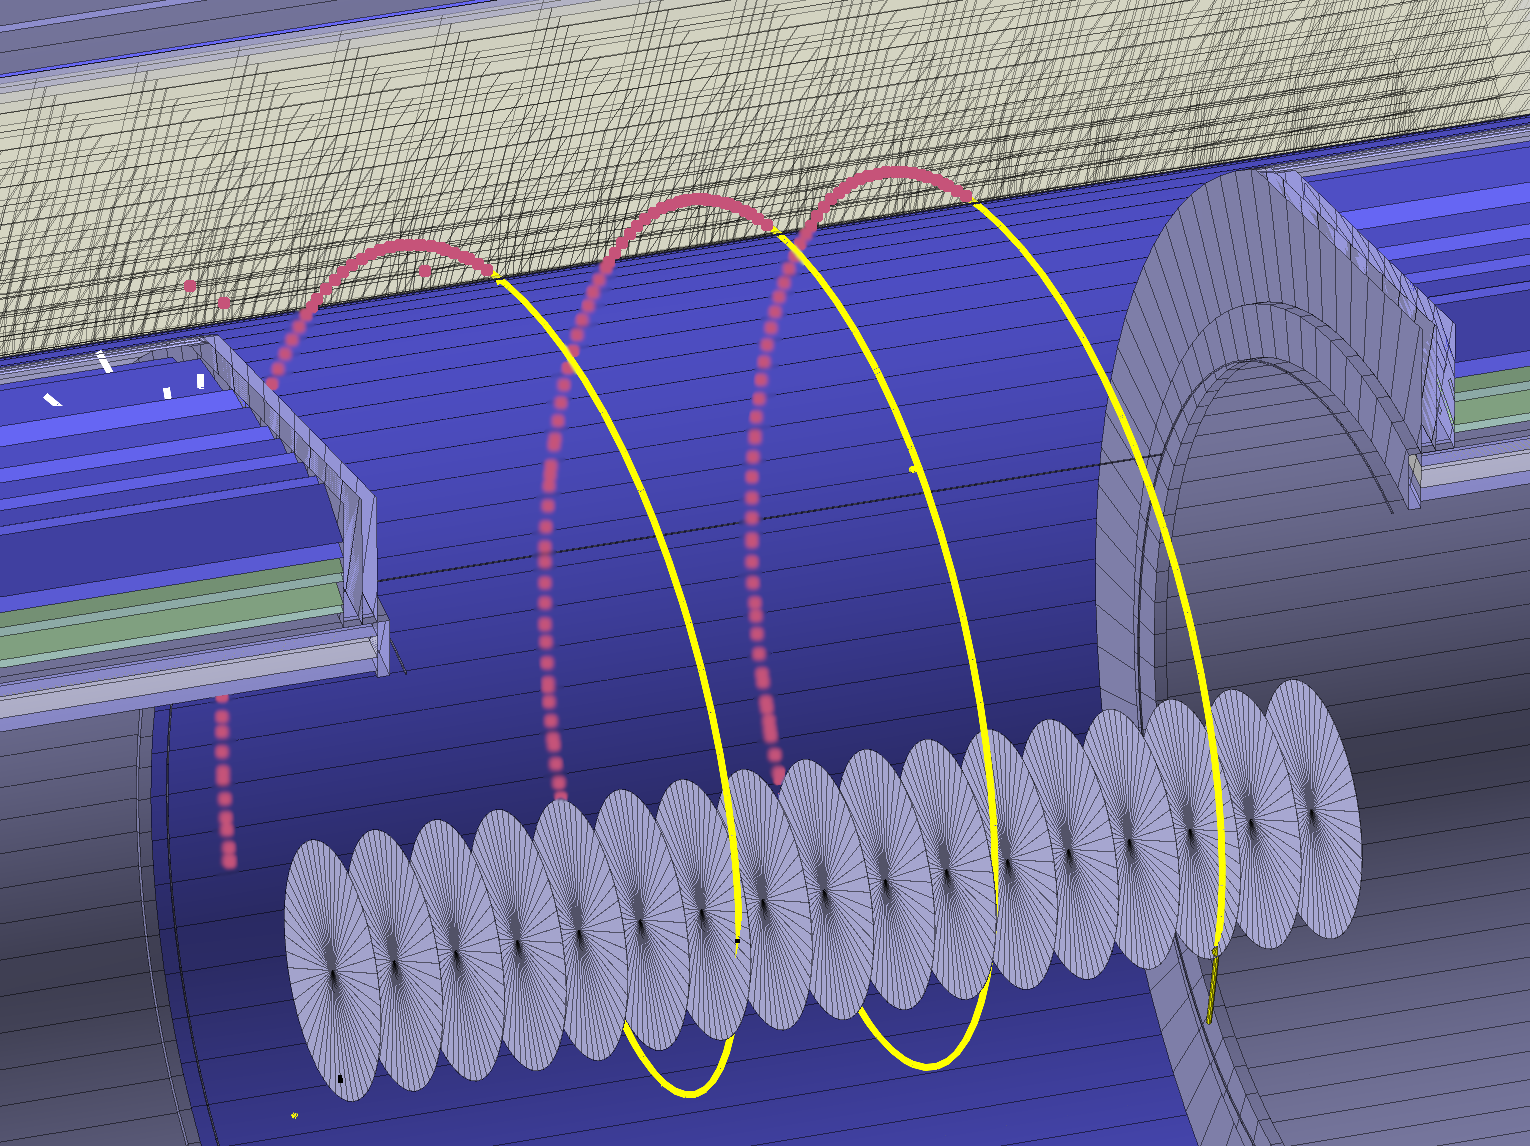
\includegraphics[width=0.5\textwidth]{chapter3/hit_instances_blur_crop.png}
    \caption{
        Hits, shown as red dots, produced by the CDC sensitive detector class
        when a particle deposits charge inside the gas. One instance of
        \texttt{IG4HitGas} is created every time the particle traverses a CDC
        cell, i.e.\ roughly every \SI{16}{\mm}.
        }
    \label{fig:sim_cdc_hits}
\end{figure}


% This new hit class and the associated algorithms were introduced to \SimG in
% 2019. 
This hit representation is designed toward gaseous detectors, hence it
also applies to the Straw-Tube Tracker of Phase-I and Phase-II. Because of the
relatively low density of hit instances along a trajectory, important details of
the true energy deposition pattern may be lost. Therefore, \SimG implements a
run-time option to store \emph{auxiliary points} inside each hit instance, which
provide a more fine-grained description of the particle's steps inside the cell.

% The \texttt{IG4HitGas} class was designed to condense and record energy loss
% information inside gaseous ionisation detectors in \SimG (e.g. the CDC and
% Straw-Tube Tracker). Every energy deposit made by a particle inside the same
% CDC cell is accumulated into a single instance of the class, such that only
% one hit per cell per particle may exist. While this saves memory and disk
% space, it limits the amount of detail that can be stored. The recorded
% information allows for basic detector response simulation, but if more detail
% is required one can tune the \SimG simulation to store finer details inside
% each \texttt{IG4HitGas} instance.



\section{Large-scale simulation: MC5}
\label{sec:mc5}
The 5th large-scale production of simulation data, MC5, was run in 2020 using
computing facilities at the French National Institute of Nuclear and Particle
Physics Computing Centre (CC-IN2P3) in Lyon, France. Using \numprint{2000}
concurrent machines over the course of a few weeks, the outcomes of 1 billion
proton-on-target (POT) collisions were simulated with \SimG in the CyDet
configuration of COMET Phase-I.

\subsubsection{Software}
Leading up to the MC5 production, several aspects of the software were changed
or updated in comparison with the previous large-scale production:
\begin{itemize}
    \item The CMake build configuration system was introduced to replace the
    legacy CMT system. 
    \item The external ROOT software, upon which the \oaEvent data format
    depends, was updated from major version 5 to 6.
    \item The CyDet geometry received multiple updates to make it as faithful as
    possible to the design, adding detailed elements such as readout boards and
    fixing errors in the positioning of CDC wires. 
    \item As discussed in Section~\ref{subsec:SD}, the treatment of energy
    deposits in the CDC was also changed to the \texttt{IG4HitGas}
    representation.
    \item All memory-related problems identified by \texttt{valgrind} at the
    time were resolved to bring the simulation software into a production-ready
    state.
\end{itemize}

\subsubsection{Run configuration}

\begin{figure}
    \centering
    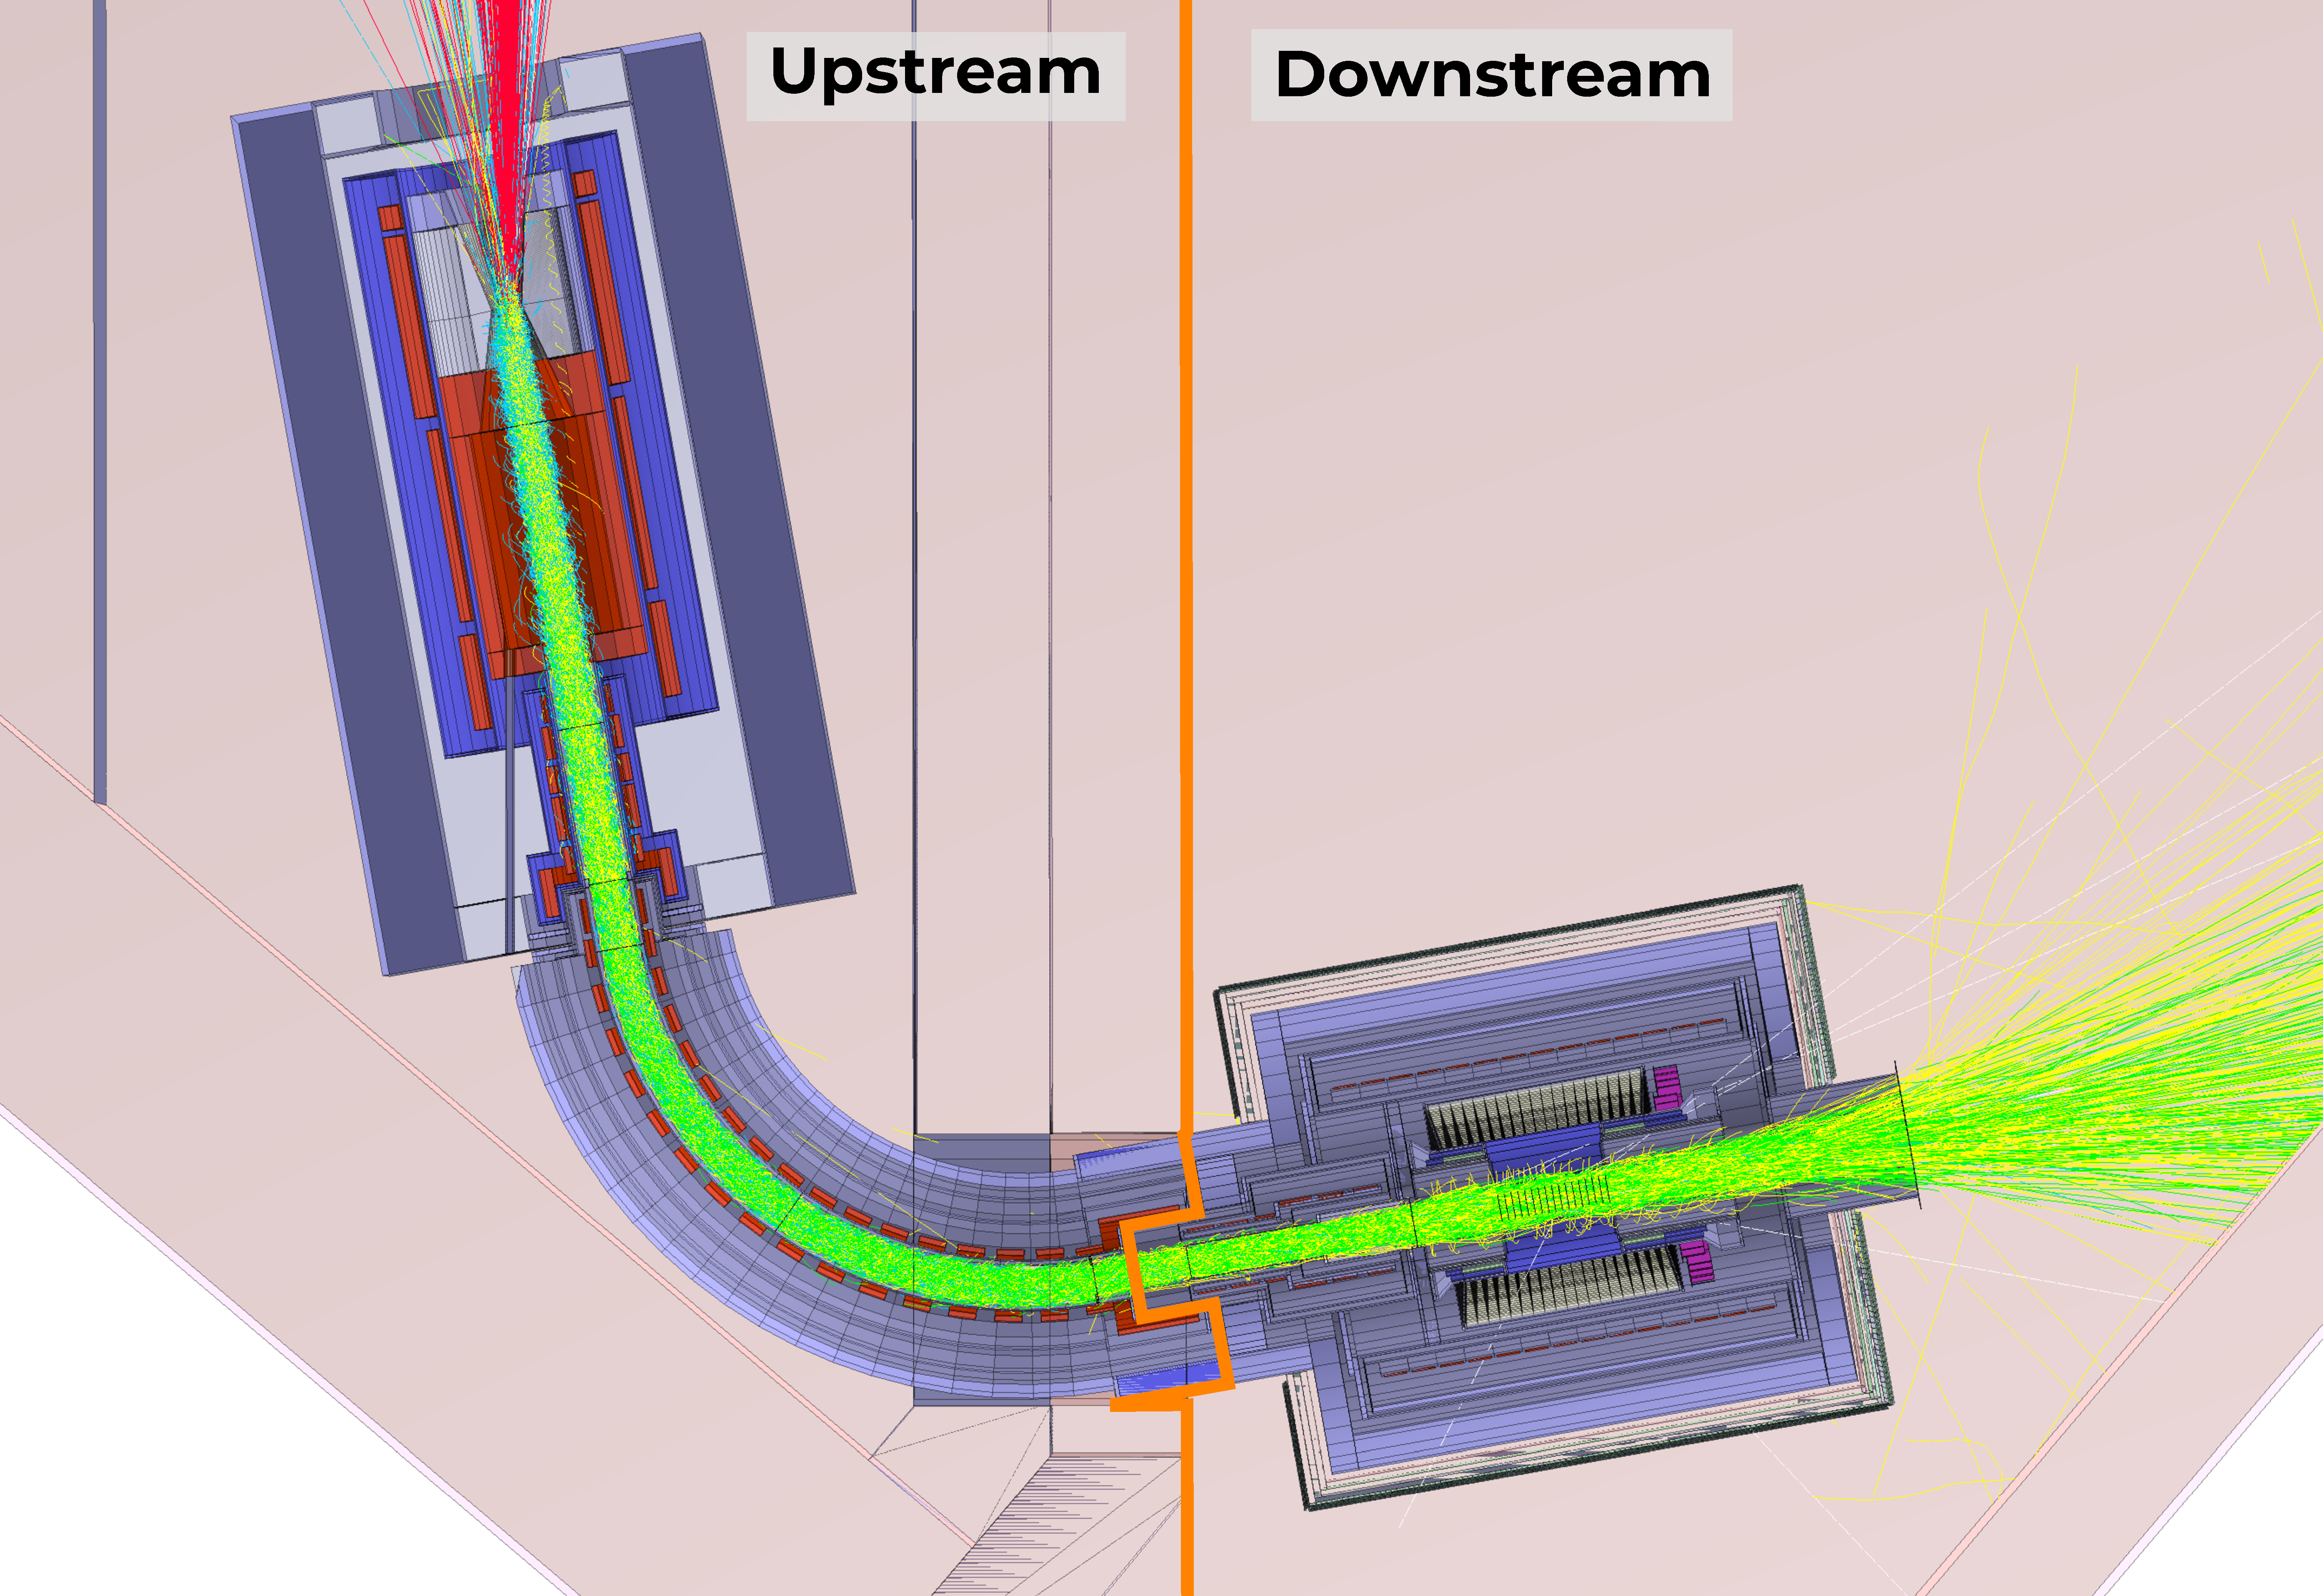
\includegraphics[width=0.6\textwidth]{chapter3/sampling_plane_illu_ink.pdf}
    \caption{
        Top-down cutaway view of the running configuration for MC5,
        showing $1.6\times 10^5$ overlaid events (1\% of a bunch). The orange
        line shows the sampling boundary where particles that cross into the
        detector region via the beamline or wall are recorded. Only
        charged-particle trajectories are shown for clarity.
    }
    \label{fig:Phase-I Sampling World}
\end{figure}



The simulation was split into two stages by dividing the world along a boundary
which effectively separates the pion-production section and transport solenoid
(\emph{upstream}) from the detector region (\emph{downstream}), as shown in
Figure~\ref{fig:Phase-I Sampling World}. The boundary is set up to record the
position and momentum of particles which enter the detector region. Most
particles will enter via the beamline, but a small fraction (mostly neutrons)
also penetrates through the wall, floor and ceiling. In the upstream run, only
particles that enter the detector region are saved to disk, along with their
ancestors. Upon doing so, their position and momentum are recorded to an
\texttt{oaRooTracker} file (see Section~\ref{subsec:RT}) which is used as input
for the downstream simulation.

This run configuration implies that the upstream simulation is unaffected by the
disposition of the detector region, hence one can perform the upstream run once
and use the results to seed multiple downstream configurations, changing the
detector geometry (e.g.\ between CyDet and the StrECAL) or magnetic field. Since
most of the simulation time is spent in the pion-production section, this gives
a flexible way to produce high-statistics MC datasets in multiple experimental
configurations.
%Another benefit is that it allows for re-seeding of the downstream run, whereby
% each event retains the same initial conditions but uses several different
% seedings of the random number generator, yielding a more diverse dataset at
% the cost of potentially biasing the sample. 
% ^ Off-topic?

\subsubsection{Outcome}
The data produced with MC5 has a total disk size of \SI{13}{TB} and is archived
on the tape storage system at CC-IN2P3. The sample size of $10^9$ POT events
represents 62 unique beam bunches when merged, or the equivalent of
$~\SI{0.1}{\ms}$ of data acquisition in Phase-I.

\section{Animated CyDet event display}
In order to visualise events in the CyDet system, a tool was developed to display
hit data from MC simulations as animations, visually similar to a slow-motion
online monitor of the detector. Figure~\ref{fig:animation} shows a series of
frames from one such animation involving a $\mu$--$e$ conversion electron.

\begin{figure}
    \centering
    
    %\captionsetup[subfigure]{justification=centering}
    \begin{subfigure}[t]{0.59\textwidth}
    \centering
    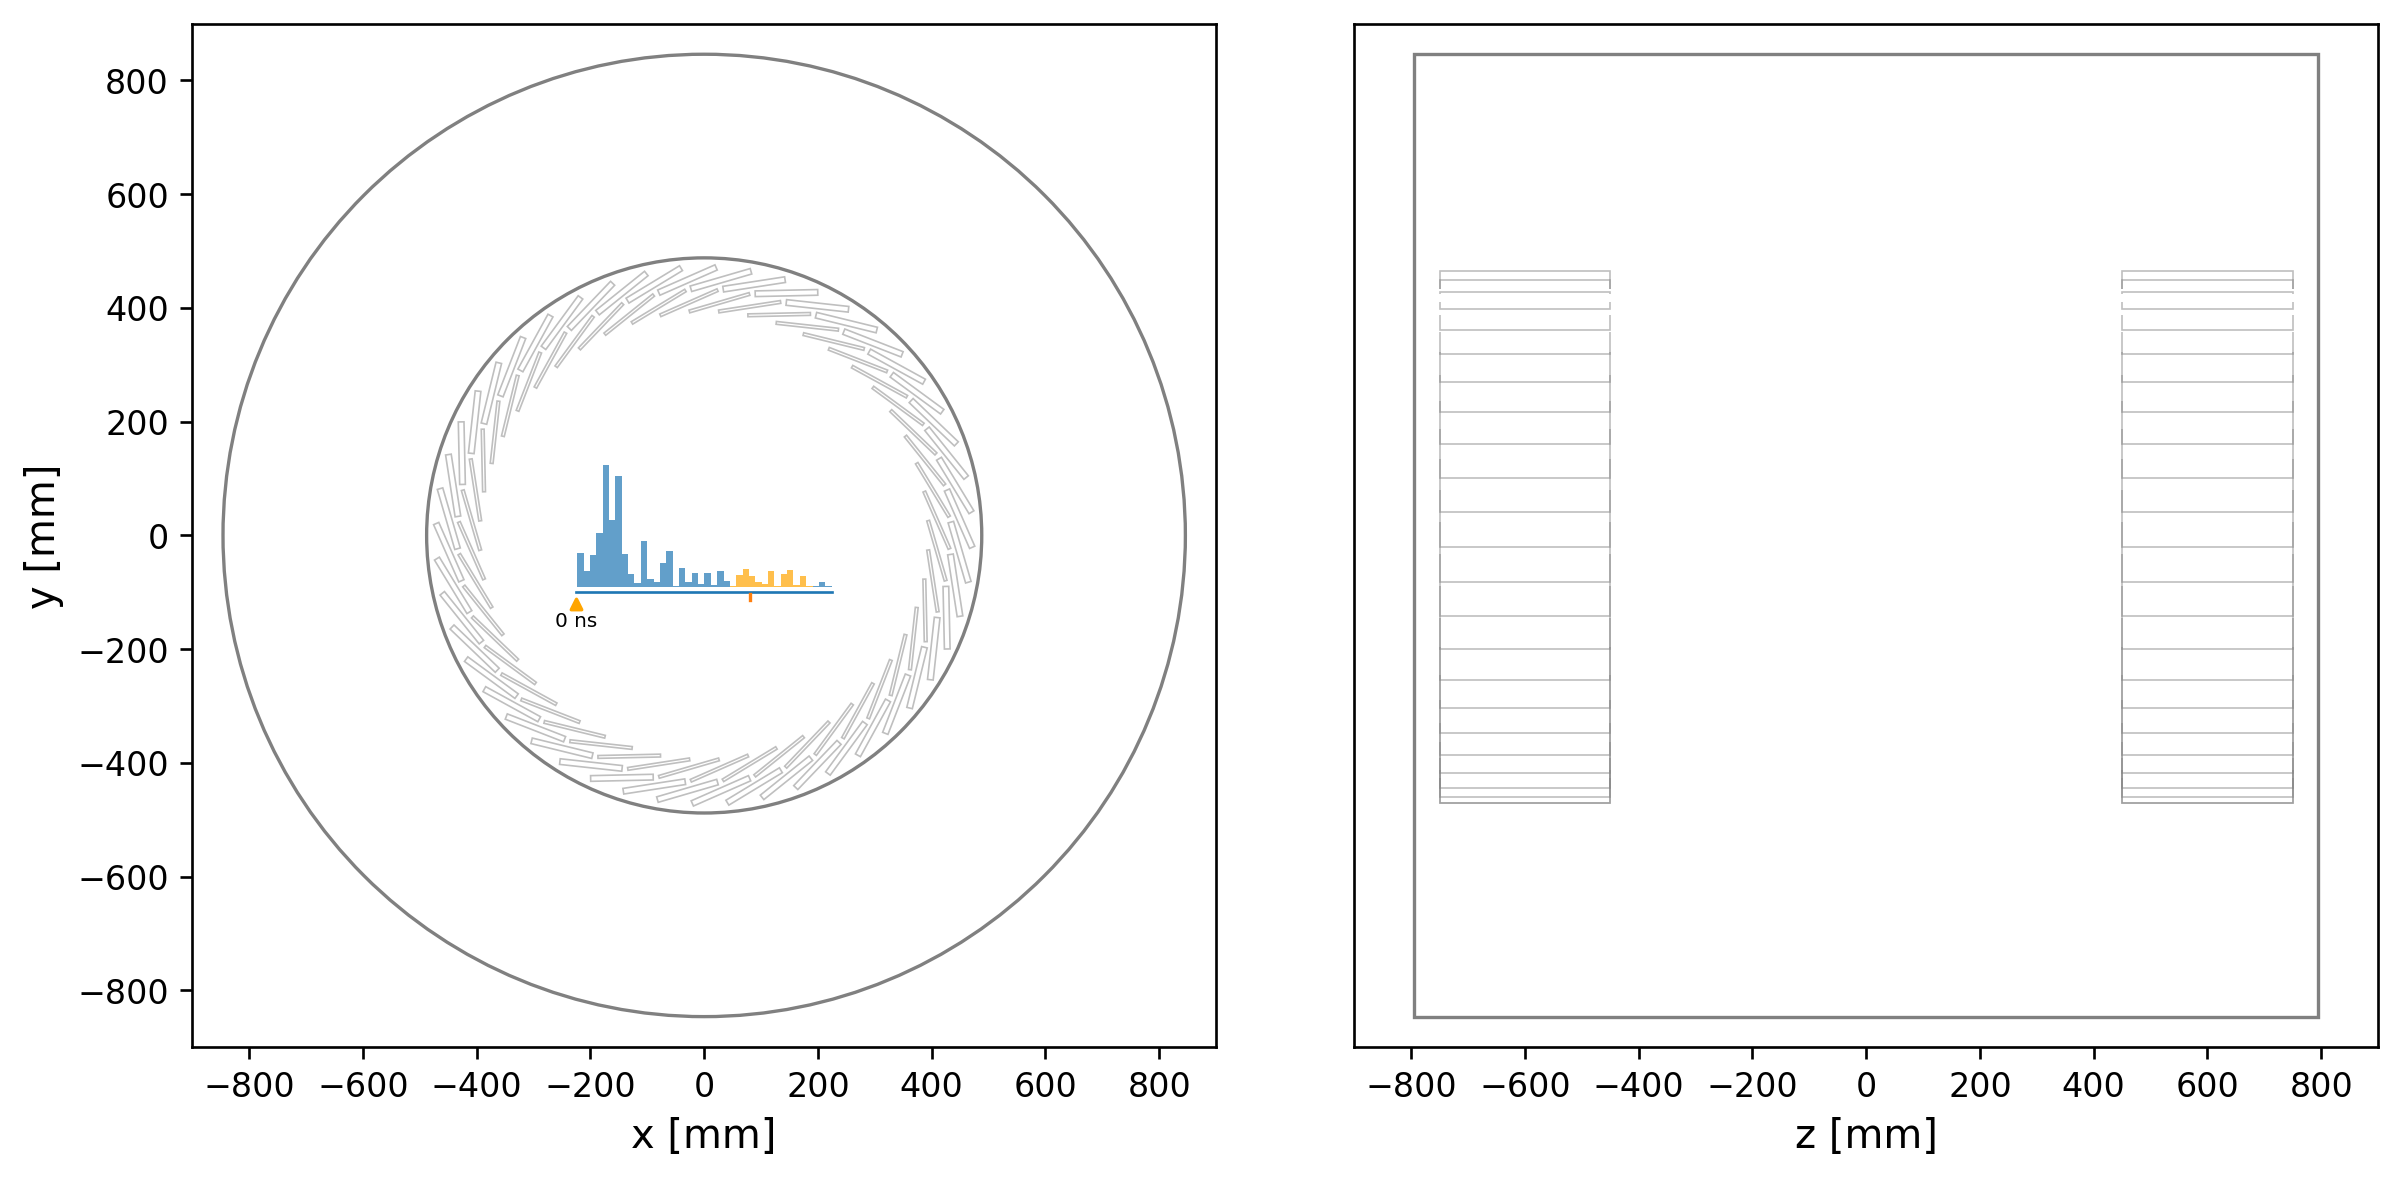
\includegraphics[width=0.95\textwidth]{chapter3/frame_005.png}
    \caption{$t=\SI{0}{ns}$. Ignoring pileup and cosmics, the detector is clear
    of hits before the POT collision.}
    \end{subfigure}
    
    \begin{subfigure}[t]{0.59\textwidth}
    \centering
    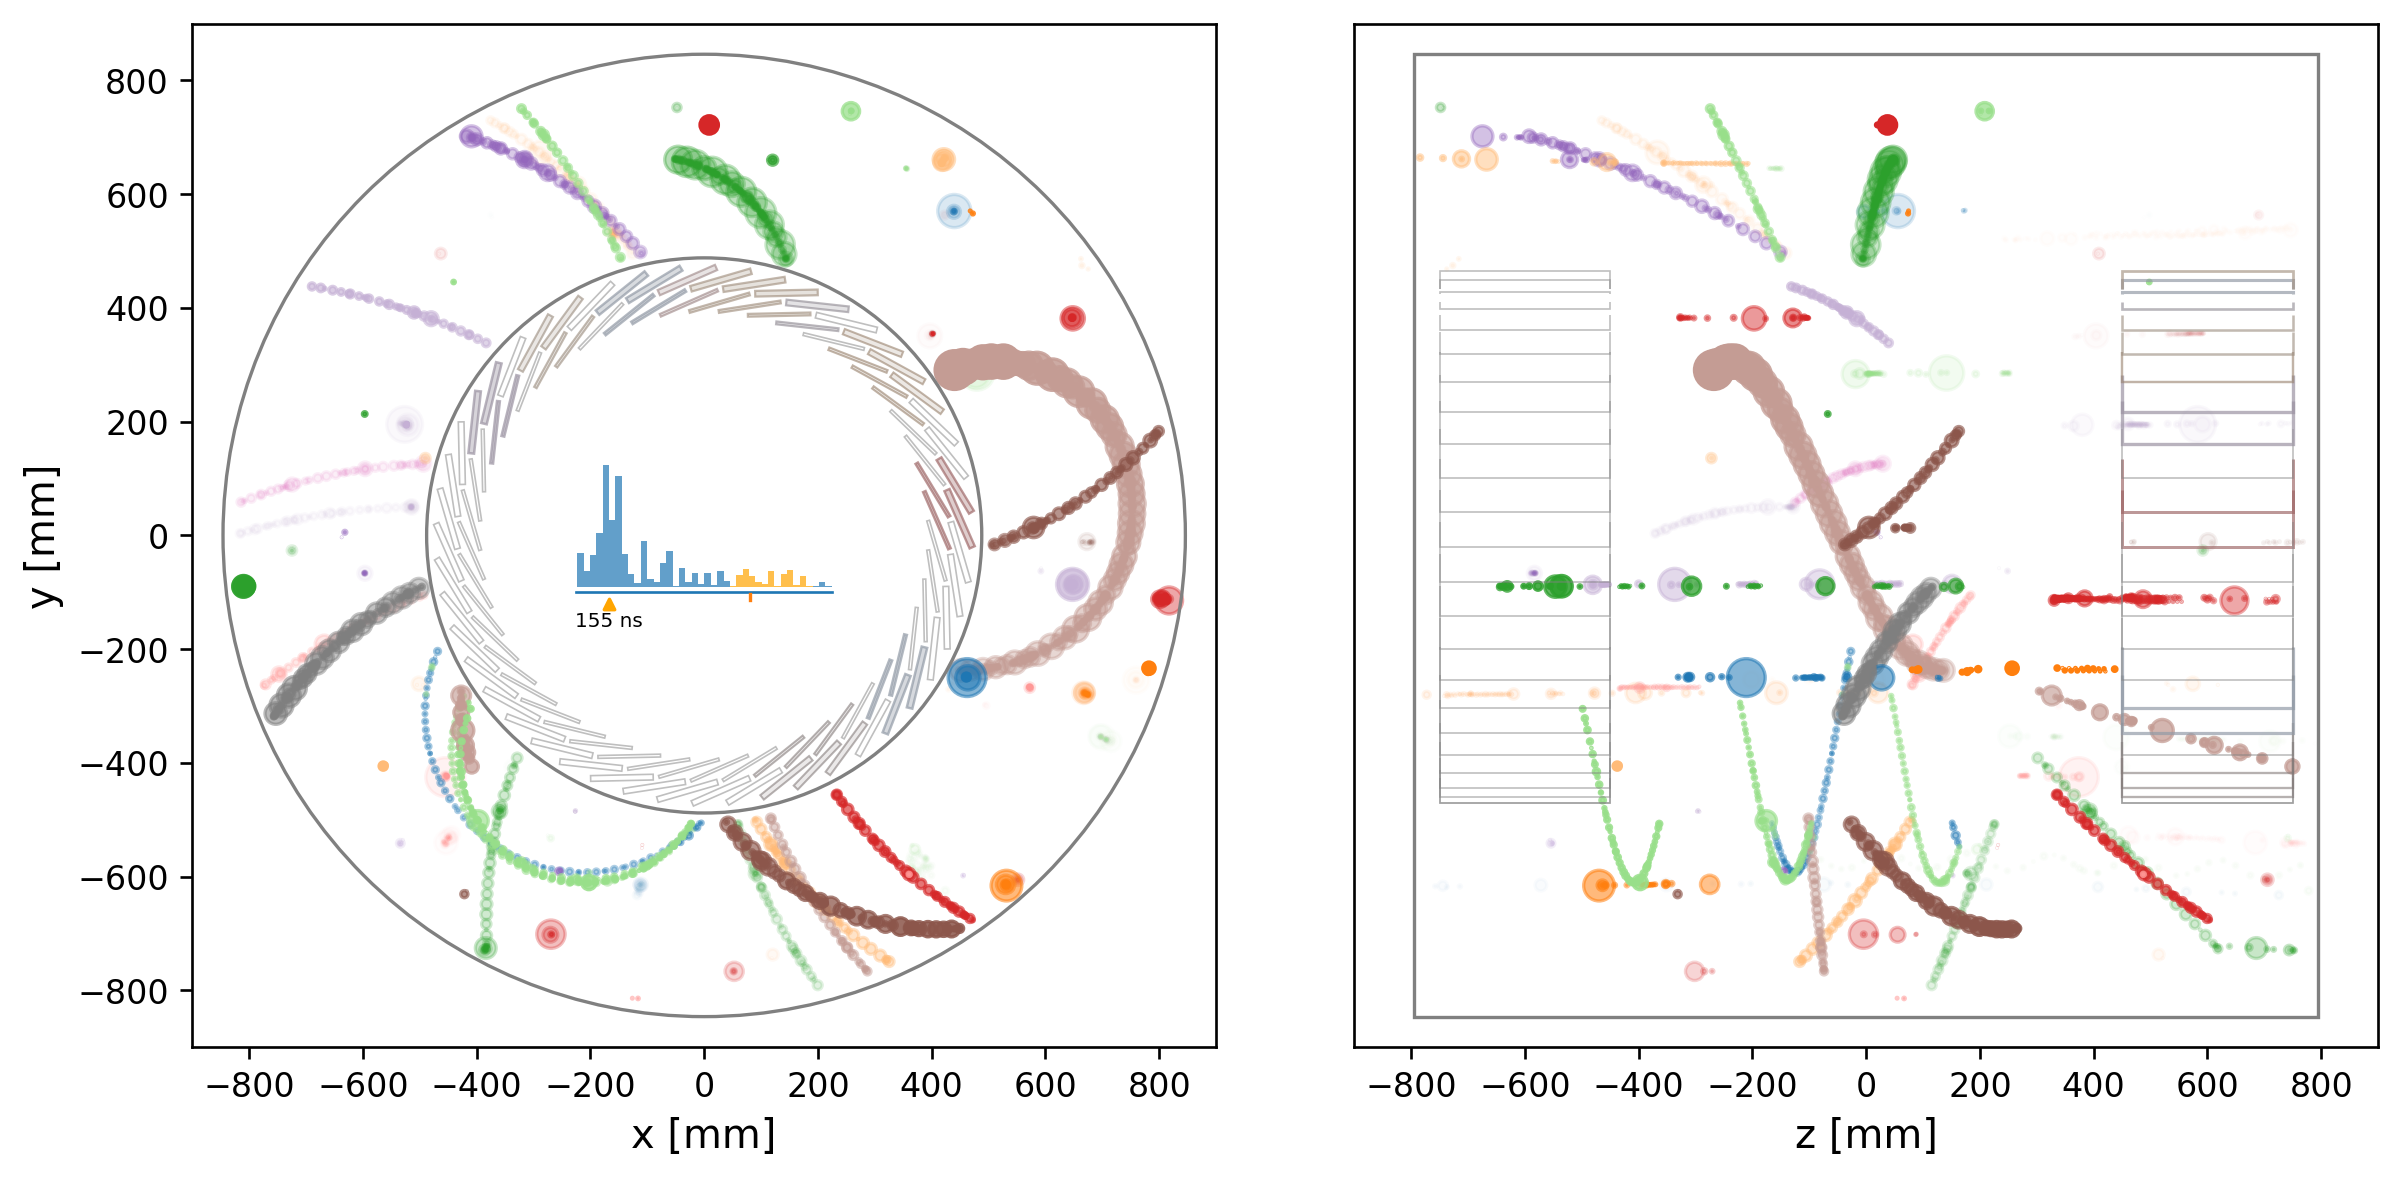
\includegraphics[width=0.95\textwidth]{chapter3/frame_036.png}  
    \caption{$t=\SI{155}{ns}$. Many tracks occupy the detector soon after the
    beam flash.}
    \end{subfigure}
    
    \vspace{0.3cm}
    
    \begin{subfigure}[t]{0.59\textwidth}
    \centering
    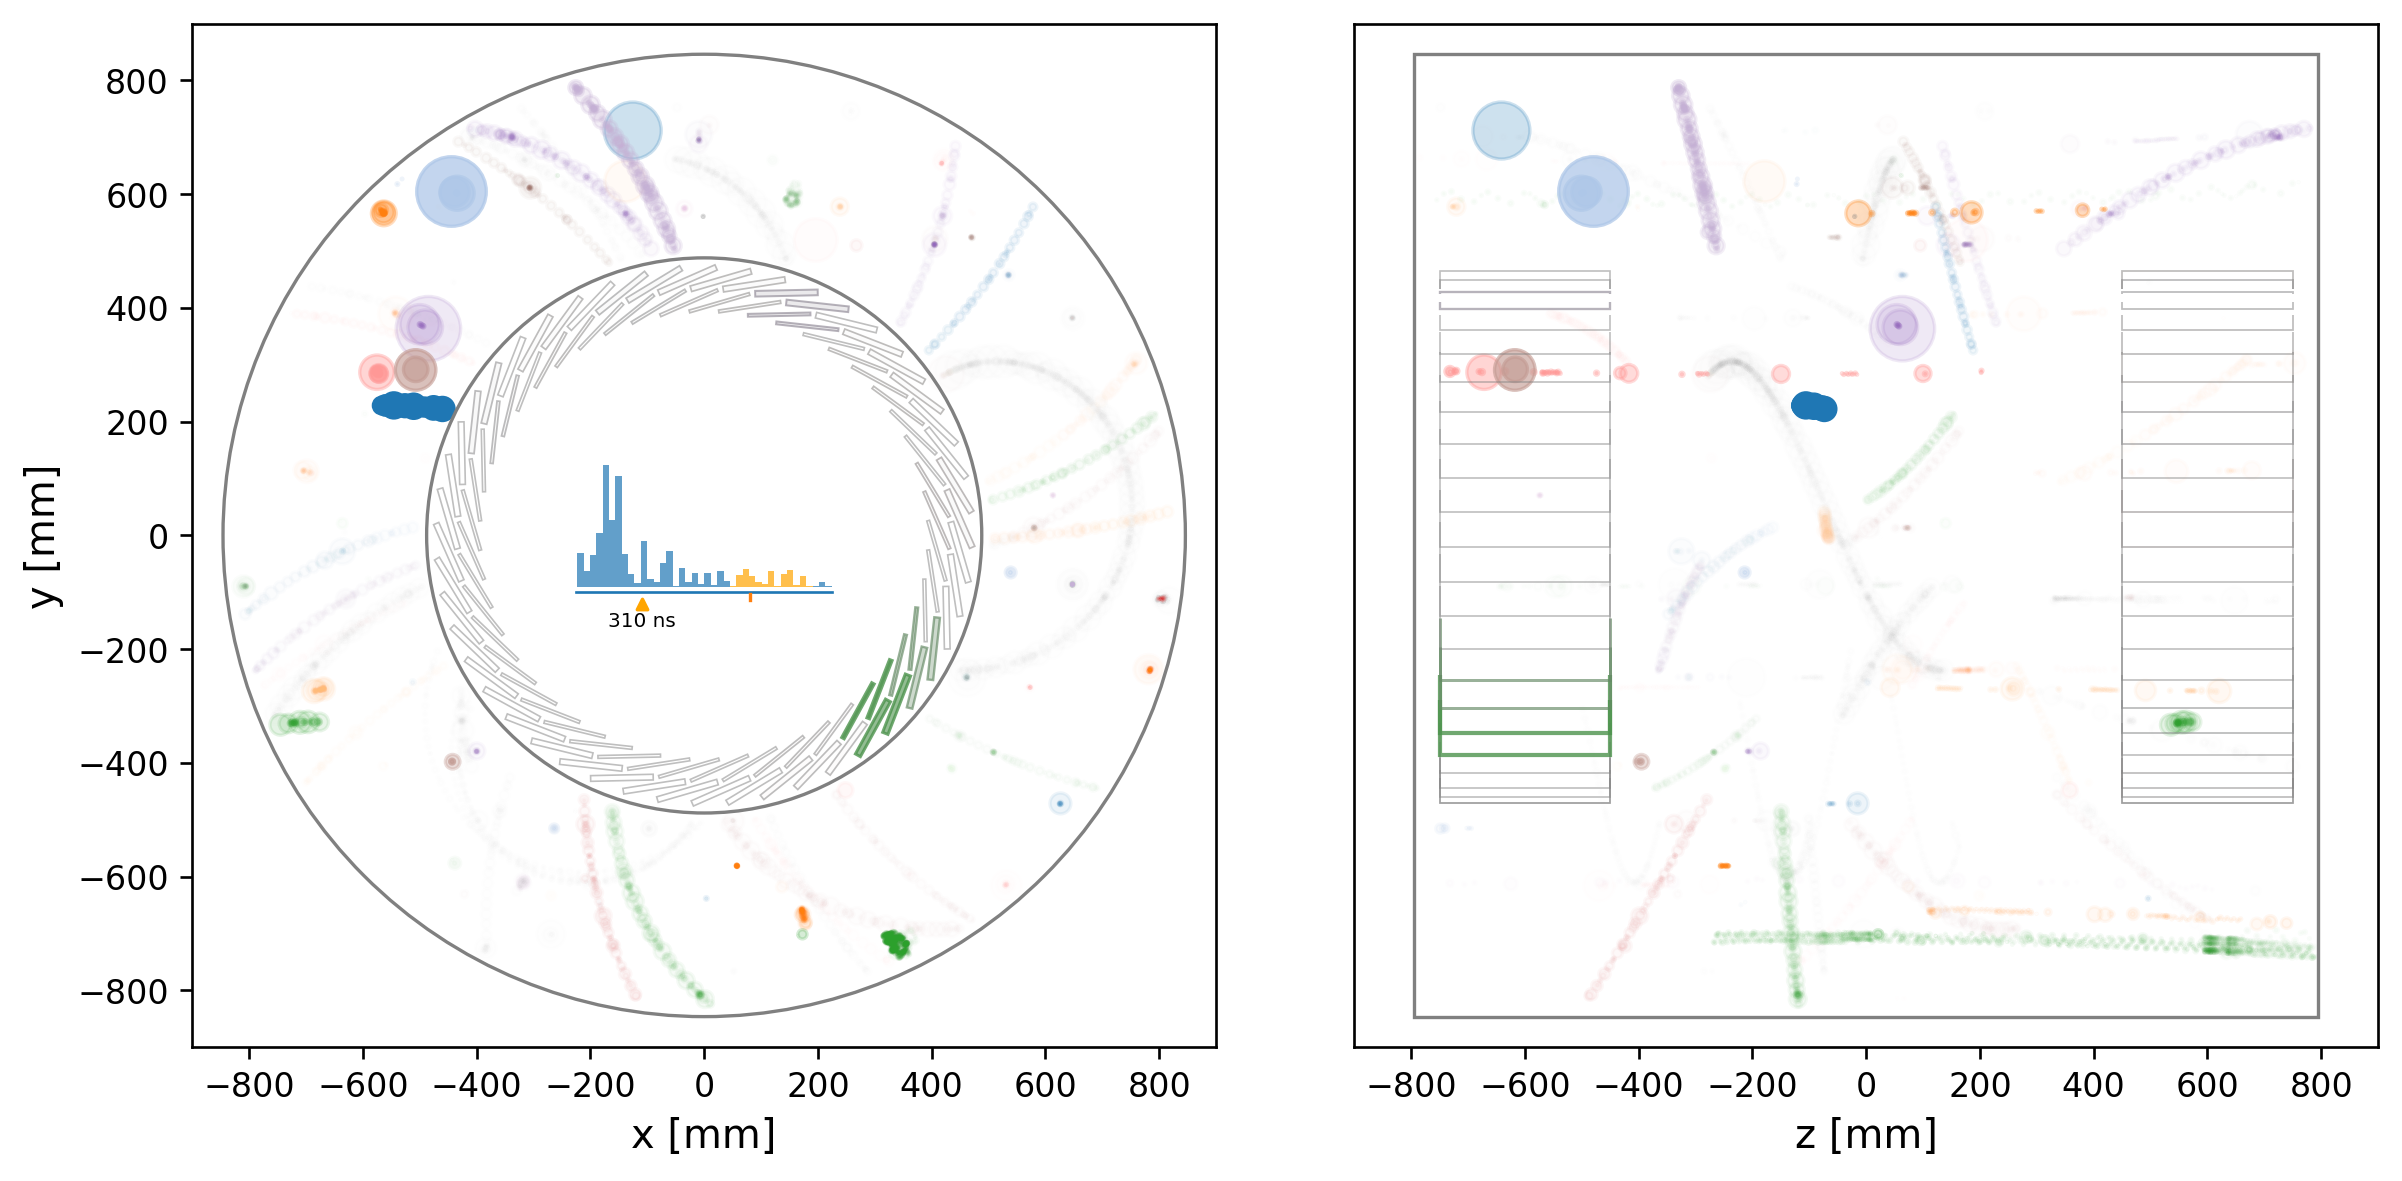
\includegraphics[width=\textwidth]{chapter3/frame_067.png}
    \caption{$t=\SI{310}{ns}$. The hit rate decreases significantly once the
    beam flash has ended.}
    \end{subfigure}
    
    \begin{subfigure}[t]{0.59\textwidth}
    \centering
    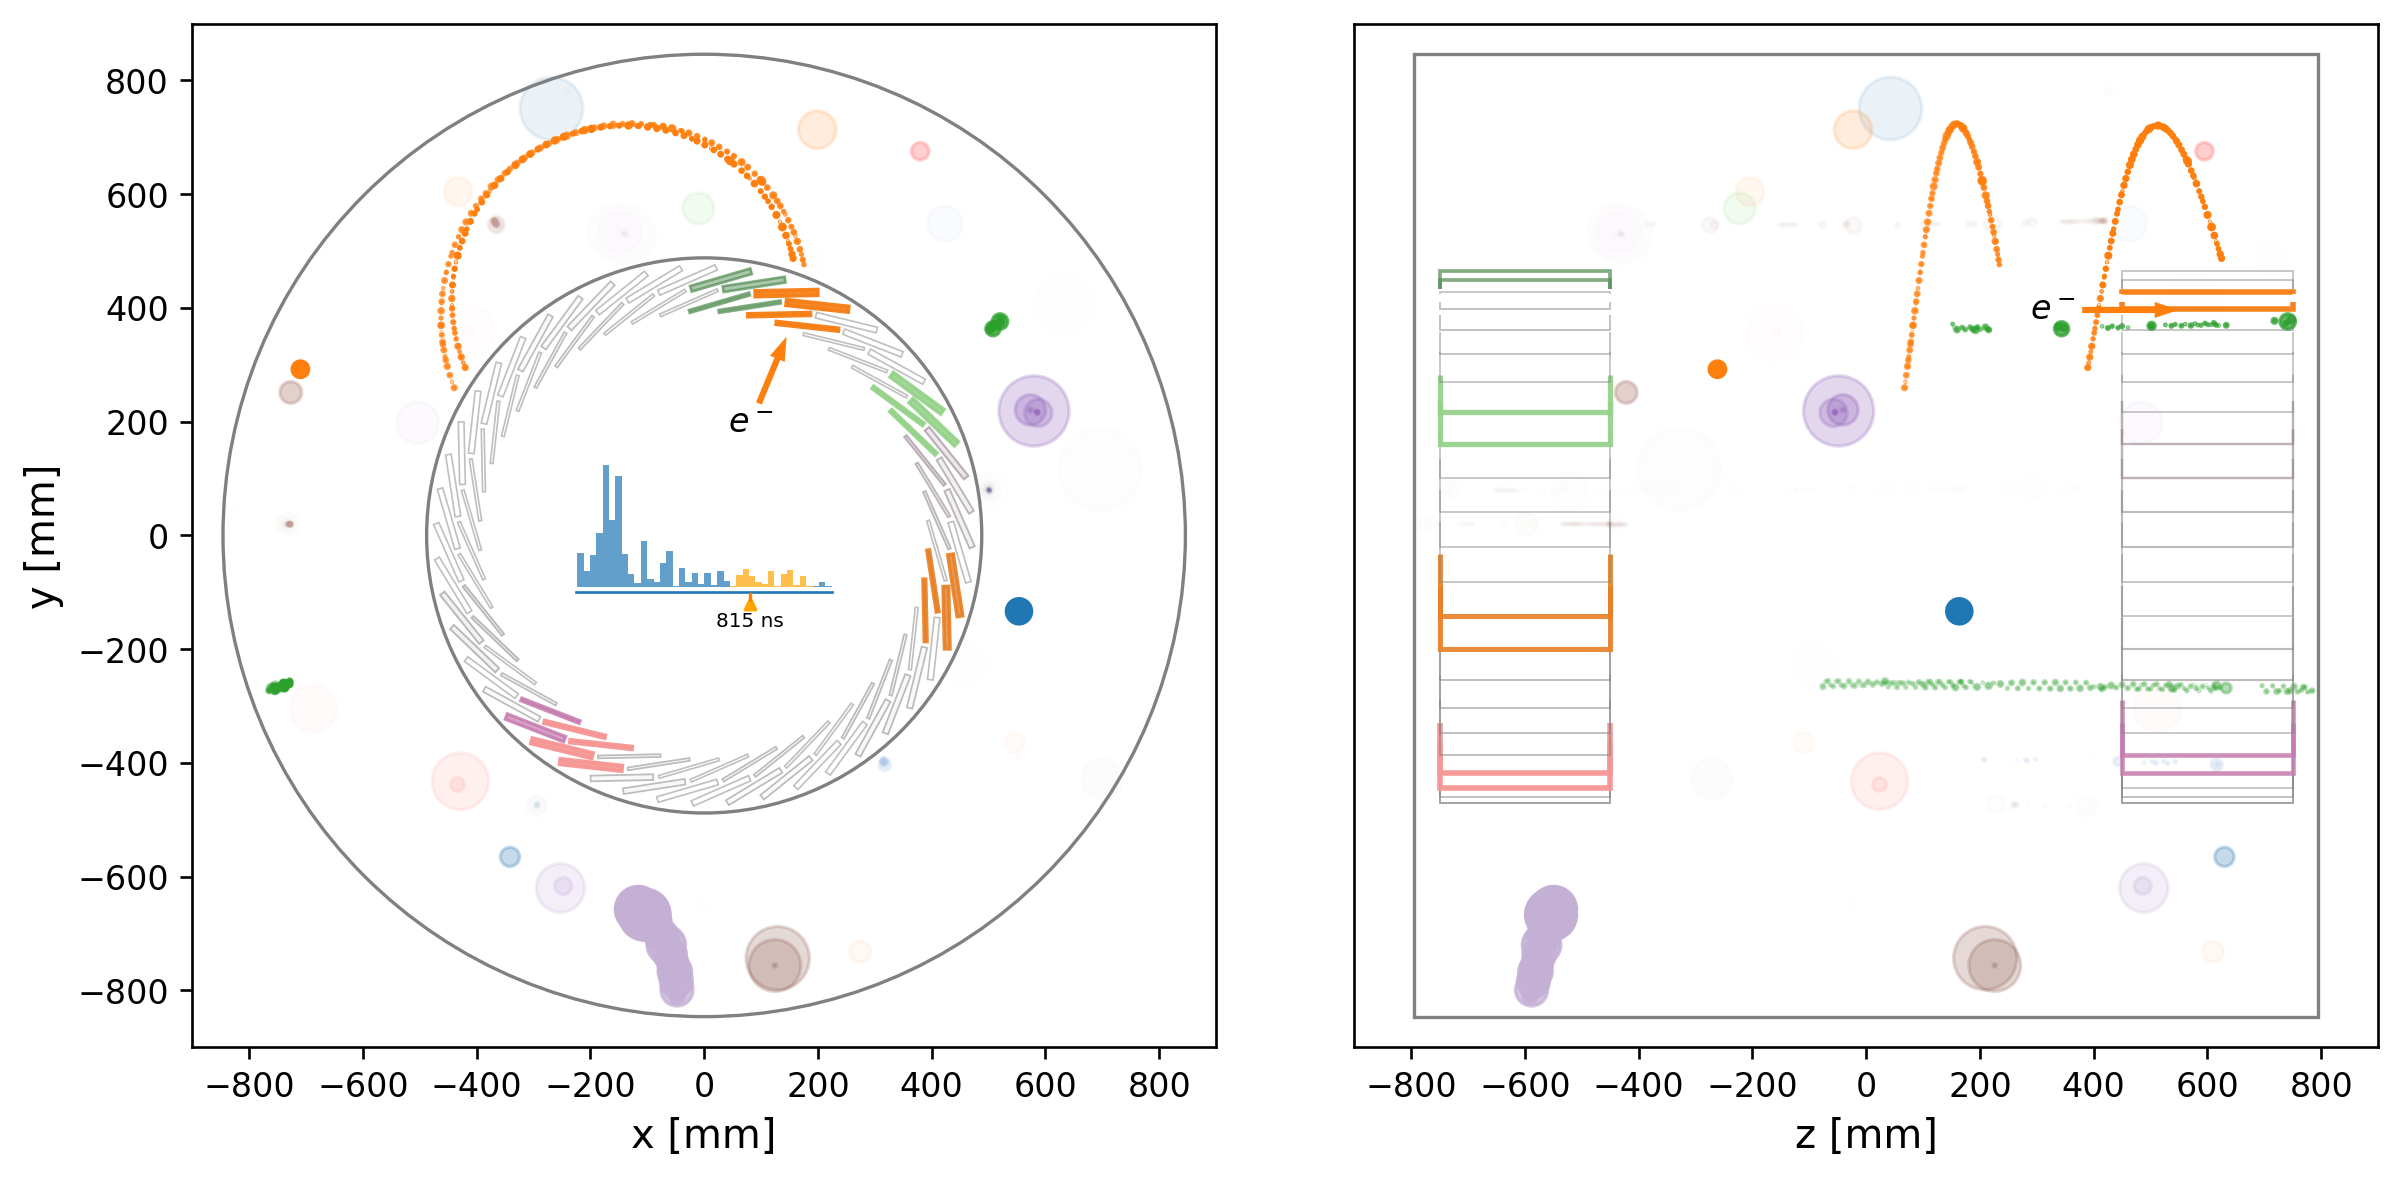
\includegraphics[width=\textwidth]{chapter3/frame_192.png}
    \caption{$t=\SI{815}{ns}$. A conversion electron appears in the CDC and
    triggers the CTH.}
    \label{fig:animation:conv}
    \end{subfigure}
    
    \caption{ Still frames of an animation rendered by the visualisation tool.
        The event shown outlines how a conversion electron would be seen by the
        CyDet system among background hits.}
    \label{fig:animation}
\end{figure}


% Visual features
The produced animations show the CyDet system under two projections such that
particle trajectories can be visualised in all three dimensions, over time. The
left-hand side of the display shows the projection in the readout plane, with
the CDC on the outside and the CTH counters on the inside, while the right-hand
side shows an orthogonal view with the same vertical axis. In the centre of the
left-hand pane, a histogram shows the rate of hits over the event's duration and
a cursor indicates the current time in the simulation.

Each animation shows one bunch event unfolding over one cycle, i.e.\
\SI{1170}{\ns} from the collision of one bunch until the arrival of the next
one. Time is slowed down by a factor of ${\sim}10^{-7}$ such that the event
unfolds over 10 real seconds.

In the CDC, the true position of every hit is drawn as a circle with a radius
proportional to the amount of energy deposited. Colour indicates hits produced
by the same particle such that tracks can be disambiguated.

The CTH counters flash only in the case of a fourfold coincidence, whereby four
adjacent counters are struck within a \SI{10}{\ns} window. Fourfold coincidences
are most often caused accidentally by multiple particles, but occasionally a
single track will hit four counters. In these occurrences, the track is
emphasised in the animation and the particle type is displayed, as shown
in Figure~\ref{fig:animation:conv}.

Hits in the CDC and CTH fade out over time such that the display does not become
too cluttered, but the fading rate is not representative of the actual time
resolution of the sub-detectors.

% Implementation details
The animation rendering tool is written in Python. The code includes an
algorithm for finding fourfold coincidences among CTH hits. To draw the frames,
it relies on the \texttt{matplotlib} package. Once the individual frames have
been rendered, a \texttt{bash} script runs \texttt{ffmpeg} to assemble them into
a video format, such as \texttt{webm}, \texttt{gif} or \texttt{mp4}.


\section{ICEDUST development}

\subsection{Version control}

The source code of the ICEDUST software project is version-controlled using Git.
A shared repository is hosted on the GitLab instance of the IN2P3, where
developers collaborate on building up and improving the code base. The
repository contains a full history of the code, an issue tracker, and a set of
wiki pages documenting the software. 

Additions and changes are submitted to the central repository through merge
requests from the developers. When submitting a merge request, changes to the
code are typically reviewed by another developer or maintainer who verifies that
no new bugs are introduced into the main branch. To further reduce the
likelihood of new issues appearing, the ICEDUST repository makes use of GitLab's
continuous integration system.

\subsection{Continuous integration and deployment}

Every time new code enters the main branch, the whole code base goes through a
three-step pipeline. The first step compiles the code and builds a new version
of every binary. The second step runs custom unit tests and validations using
this new build. Each unit test typically verifies that a single functionality
works as intended in an isolated environment, while validations can run multiple
pieces of the software and ensure that the results are consistent between one
revision of ICEDUST and the next.

If the building, unit testing and validation stages all pass, the pipeline moves
to the final deployment step where the new binaries are assembled into a Docker
image which is published to the repository's container registry. Users who wish
to use the compiled software as-is can download this image and run it via Docker
or Singularity. If any of the pipeline steps reports a failure, the developer
submitting the merge request is notified and full logs are provided to identify
the issue. A merge request is usually only accepted once the code has been
reviewed and if the pipeline finishes successfully.

\subsection{Documentation}
ICEDUST uses Doxygen to generate documentation of the source code. Doxygen
parses the C++ code and comments to produce a set of static HTML pages
containing types, functions and inheritance diagrams that can be navigated in a
web browser.

In order to automate this process as the software evolves over time, the
generation of the documentation was added as a step in the deployment stage of
the continuous integration pipeline. Whenever a merge request is accepted,
Doxygen is run on the updated code base to generate a new set of web pages
containing the source code reference. This content is then pushed to the
built-in \emph{Pages} of the ICEDUST repository, a static web server hosted on
the GitLab instance alongside the Git repository and wiki pages. This then
provides a central, always up-to-date version of the documentation that all
developers and users can access and use as reference.




\chapter[Data Augmentation with Generative Adversarial Networks]{Data
Augmentation with \\ Generative Adversarial Networks}
\label{ch:gan}
% \begin{markdown}
% ---

% - We are coming from the simulation chapter, so:
% - Problem description: 
%  - We would like to produce larger amounts of simulation data, e.g. for a mock
%    dataset in preparation for data-taking
%  - But we have limited capability to produce MC data with simulation. The main
%    bottleneck is in the pion-production section's hadronic interactions. Is
%    there a faster way?
%   - The topic of this chapter is to consider the application of
%     machine-learning methods in the fabrication of fake Monte Carlo data.


% - Creation of dataset from Monte Carlo simulation
%   - Hit pattern characterisation
%   - Reconstructible vs noise-like classification
% - GAN theory [Goodfellow, WGAN, WGAN-GP]
%  - Pre-processing
% - GAN design, basic architecture, softmax for classes [WGAN-GP]
% - GAN extensions, embedding? analogy with text?

% ---
% \end{markdown}

% Need to wrap the start of this chapter into a compelling narrative:
% 1. MC allows us to see possible patterns in detector sys e.g., in CDC,
%    high-mom tracks produce structured hits whereas low-mom make small
%    localised hit clusters --> Draw figures
% 2. For an exercise such as a mock-data challenge (explain term), traditional
%    MC is not efficient enough to produce the dataset.
%  + Think about: why do we want mock data? Why is the standard sensitivity
%    estimation process not sufficient?
%    - Perhaps the extrapolation factor. Considering efficiencies on a limited
%       sample cannot effectively be representative of the real situation.
%    - The sheer sample size makes the exercise worth it? Test limits of the
%       data processing chain and increase preparedness for real situation.
% 3. Now consider the problem of producing artificial / fake / imitation /
%    fictitious / fabricated data.
%  + Consider alternatives
%  + Introduce GAN for detector-level data fabrication.


% v -- This intro is plain useless I think. 
%As discussed in the previous chapter, Monte Carlo simulation allows us to draw
%a realistic picture of what will happen in our experimental setup once it is
%running. Most importantly, it provides an estimate of the kinds of patterns we
%can expect to observe in the detector system. 

When performing a full simulation of COMET Phase\nobreakdash-I, most of the activity takes
place in the initial collision between the proton beam and the graphite target.
The many hadronic interactions caused by the proton beam collision
represent \SI{99.7}{\percent} of the computational cost of the Monte Carlo
simulation.
In addition, because of the large distance between the pion production section
and the detector area, only about one POT collision in a thousand will produce
observable hits in the detector system. 

Hence, despite being the most physically
accurate means to synthesise data in the detector, simulating each proton
individually is also very computationally inefficient. Using this brute-force
method with the infrastructure used for MC5, it is only possible to produce the
equivalent of 100 to \numprint{1000} beam bunches, which is far from the $2\times 10^{12}$
expected bunch collisions of COMET Phase\nobreakdash-I.


% Calculation of MC5 simulation "efficiency" We can
% RooTrackerTree->Draw("StdHepN", "StdHepN>0") to get the number of events with
% a downstream track, but to get the number of events with a hit, it's a bit
% more involved... We need to use the downstream root files MC5A01: StdHepN>0
% --> 27267993 / 990678400 ~= 2.75% in all RT files ---> 2.75% of all POT events
% lead to >=1 particle entering the detector region Repeat on MC5A02 RT files to
% get stopped muons per POT MC5A02: StdHepN>0 && StdHepPdg==13 --> 486051 /
% 990678399 ~= 0.049% ---> 0.049% of all POT events lead to >=1 stopped muon
% /sps/mc5a02/count_events_with_cdc_hits.C --> 5939 / 4980700 ~= 0.12% in first
% root file /sps/mc5a02/count_events_with_cdc_hits.C --> 1173800 / 990678399 ~=
% 0.1185% in all dataset Watch job 20862516 output for answer ---> 0.12% of all
% POT events lead to >=1 hits in the CDC CORRECTION: we counted events where
% there are hits even if none of them have edep>0 --> Only count events where at
% least one edep>0 hit occurs: /sps/mc5a02/count_events_with_cdc_hits_edep.C -->
% 260 / 4980700 ~= 5.22e-5 in first root file in first 10: 2611 / 49468900 ~=
% 5.278e-5 extrapolate to all = 52289 / 990678399

% v -- If we need detail on how long one POT/bunch/Phase-I takes to simulate: On
%average, simulating a single POT event in the upstream region requires
%\SI{2.73}{\second}. A single proton bunch contains \num{16000000} protons,
%which, if simulated linearly would take 500 days of computation. The MC5
%production ran for around two weeks on 2000 concurrent machines in order to
%fully simulate 62 bunches, around $1\times10^9$ protons. During the data-taking
%period for COMET Phase-I, $2\times10^{12}$ bunches, or $1.6\times 10^{19}$
%protons, are expected to hit the target. Simulating a similar amount of MC data
%is simply impossible with the same methods and infrastructure used to produce
%MC5.

% Why would we want to do that though? Does anyone else do it? Asked Joe Joe
% says: they only really care about signal MC, MC of just background seems
% pointless to them... Because they weigh events: they have a rough idea, from
% event generators, of how likely any event is. Our approach is more
% brute-forcey. 

% Before talking about why it's impossible, we need to bring up the fact that we
% WANT to get that much data. We need to motivate this... Mock-data In COMET,
% one event could make the difference between absence of signal and CLFV
% discovery. Because of the beam transport, it is hard to estimate the kinds
% background that can enter the detector system. -> MC is heavily used to
% constrain or estimate the rates of various background processes


\subsubsection{Efficient sampling methods}
In order to produce detector-level data more efficiently, the outcomes of a full
MC simulation can be re-used to generate events. Generally, any sampling
mechanism which enables us to forego the proton collision will make the
simulation more efficient at the cost of more uncertainty in the outcomes.

In the MC5 simulation described in Section~\ref{sec:mc5}, particles
entering the detector region (either via the beam pipe or through the walls) are
frozen and saved to disk to be processed later. These saved states can be reused
by propagating them with multiple distinct random seeds, thus affecting the outcome
of every interaction and augmenting our sample.

Another way of generating events closer to our region of interest is to
histogram the kinematics of particles at a given boundary and then sample events
from the estimated distribution. In ICEDUST, the \texttt{oaRooTracker} format
used to store particle states (see Section~\ref{subsec:RT}) can be aggregated
into histograms, which are then used as input by the simulation.

% v Cool idea for further studies Alternatively, particles produced in the
%hadronic interactions which have a small probability of resulting in observable
%detector hits could also be aggressively culled, at the risk of potentially
%suppressing important events. To eliminate particles, a straightforward
%algorithm cutting on position, momentum and particle type might suffice, but a
%more intelligent classifying algorithm (e.g.\ a decision tree) which uses these
%features and others could improve the selection efficiency. 


To optimise the efficiency of the simulation even further,
%(i.e.\ the likelihood for any event to induce detector hits)
one could sample hits directly inside the detector system. In this chapter, we
consider a fast generator of hit data to supplement Monte Carlo simulation.
This generator should replicate hit patterns produced by simulated particles in
the detector, without relying on a full particle-by-particle tracking approach.

% v Can remove? In this chapter, I will discuss my implementation of a
%Generative Adversarial Networks-based solution to the problem of augmenting CDC
%hit datasets. This restricted application ultimately strives toward a
%CyDet-wide event sampling algorithm whose lower computational cost compared to
%traditional Monte Carlo simulation would enable the production of larger
%datasets, on a scale approaching that of the Phase-I data-taking run.


\section{Generative Adversarial Networks}
Generative Adversarial Networks (GANs) are a class of generative models that can
learn the underlying distribution of a dataset in order to synthesise new
samples~\cite{goodfellow_generative_2014}. Training a GAN requires two neural
networks to compete in a zero-sum game where one network (the \emph{generator})
generates samples and the other (the \emph{discriminator}) tries to discriminate
between real and generated data. Figure~\ref{fig:gan_diagram} schematically
illustrates a generic GAN training procedure.


As the conventional example, let us consider the case where both the
discriminator and the generator are implemented as multi-layer perceptrons,
denoted as $D$ and $G$ respectively. 
The discriminator $D$ is designed as a binary classifier whose goal is to tell
real samples (from the \emph{training} dataset) apart from fake (generated)
ones. Given a sample $\bm{x}$, it outputs a score between 0 and 1, i.e.\ 
$D(\bm{x}) \in [0, 1]$. Similar to a classification task, we define the loss
function of $D$ as the cross entropy between its prediction and the true label
(conventionally, 0 for a fake sample and 1 for a real sample):
\begin{equation}\label{eq:D_loss}
    \mathcal{L}_D =
    -\mathbb{E}_{\bm{x} \sim p} [ \log D(\bm{x}) ] -
    \mathbb{E}_{\tilde{\bm{x}} \sim g} [ \log( 1 - D(\tilde{\bm{x}}) )],
\end{equation}
where $\mathbb{E}$ denotes the expected value or mean, $p$ is the distribution
of real samples and $g$ is the distribution of samples generated by $G$.
Minimising this function with respect to $D$ implies that the discriminator will
tend to assign a high score to samples drawn from the training dataset and a low
score to generated samples.


\begin{figure}
    \centering
    \hspace{-2cm}
    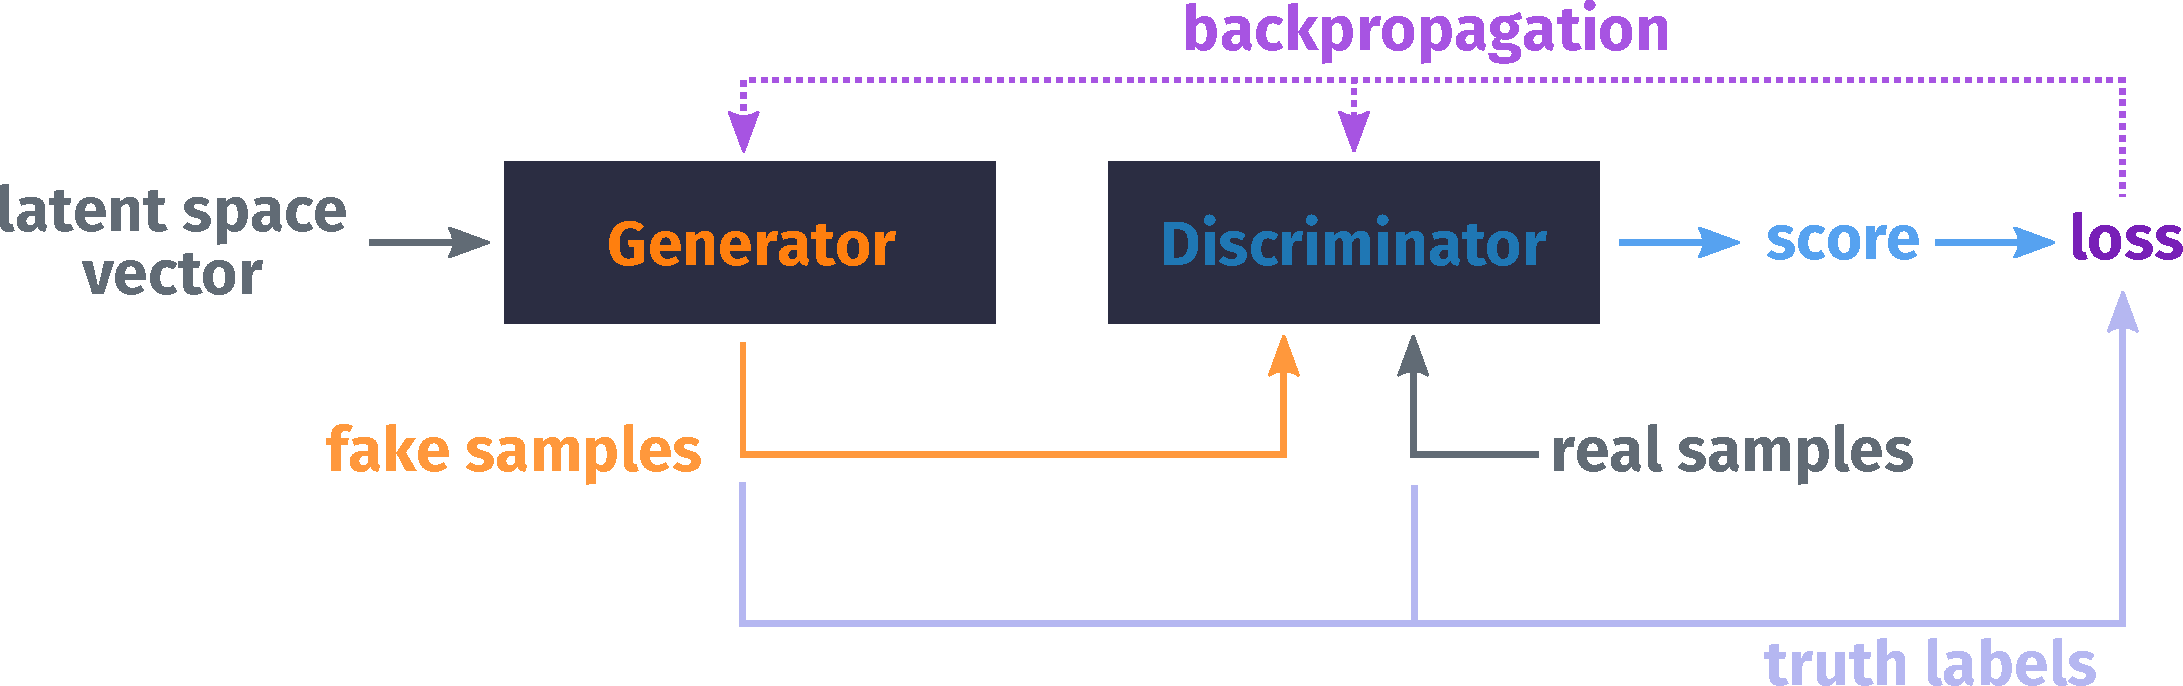
\includegraphics[width=0.75\textwidth]{chapter4/gan_diagram.pdf}
    \caption{
        Schematic diagram of the data flow in the GAN training procedure. Real samples from the training dataset and fake samples from the generator
        are iteratively evaluated by the discriminator to compute a score. The loss for
        both networks is estimated by comparing the score to the sample's associated
        truth label (real or fake). By \emph{backpropagation}, the loss is then
        numerically differentiated with respect to the network weights. The
        weights are then adjusted in the direction of decreasing loss.
    }
    \label{fig:gan_diagram}
\end{figure}


The generator produces fake samples by mapping vectors from a latent space into
data space. Latent-space vectors $\bm{z}$ are sampled according to a prior
$p_{\bm{z}}(\bm{z})$, typically a multivariate normal distribution for
simplicity and speed. The objective of $G$ is to generate samples
$\tilde{\bm{x}} = G(\bm{z} \sim p_{\bm{z}})$ such that
$D(\tilde{\bm{x}}) \rightarrow 1$. In other words, the generator aims to
maximise the second term in Equation~\ref{eq:D_loss}, and its loss function is
\begin{align}\label{eq:GAN_gen}
    \mathcal{L}_G & =
    \mathbb{E}_{\tilde{\bm{x}} \sim g} [ \log( 1 - D(\tilde{\bm{x}}) )]\nonumber        \\
                  & = \mathbb{E}_{\bm{z} \sim p_{\bm{z}}} [ \log( 1 - D(G(\bm{z}) )].
\end{align}

Combining these minimisation tasks, we obtain the mathematical formulation of
the adversarial training objective:
\begin{equation}\label{eq:GAN}
    \min_G \max_D \quad
    \mathbb{E}_{\bm{x} \sim p} [ \log D(\bm{x}) ] +
    \mathbb{E}_{\bm{z} \sim p_{\bm{z}}} [ \log( 1 - D(G(\bm{z}) )].
\end{equation}
Although it is not a formal requirement, using neural networks for $D$ and $G$
allows the above minimax solution to be approximated via backpropagation and
stochastic gradient descent. At every iteration, we evaluate the gradient of
each loss with respect to the internal weights of its respective network. Every
weight is then adjusted toward the direction of steepest decrease in the loss.



\subsection{Wasserstein GAN}
% WGAN, WGAN with Gradient Penalty
The original formulation of GANs is notoriously difficult to train due to either
non-convergence, instability or mode collapse\footnote{Mode collapse is the
situation where $G$ maps every point in the latent space onto the same output,
leading to low diversity in the generated samples.}. Training a GAN model is
highly sensitive to the choice of hyperparameters: learning rate, optimisation
algorithm, network architecture.

The Wasserstein GAN (WGAN) formulation is an attempt to address the stability
issues of the original GAN~\cite{arjovsky2017wasserstein}. The authors argue
that solving Equation~\ref{eq:GAN}, which implicitly minimises the Jensen-Shannon
divergence between $p$ and $g$, leads to vanishing gradients when the
discriminator is too powerful, and thus to unstable training. Instead, they
propose to minimise the Wasserstein-1 distance between $p$ and $g$ because of
the superior continuity and differentiability properties of that metric. They go on to show
that if the discriminator is 1-Lipschitz continuous, then the adversarial
training problem can be formulated as:
\begin{equation}
    \min_G \max_D \quad
    \mathbb{E}_{\bm{x} \sim p} \left[ D(\bm{x}) \right] -
    \mathbb{E}_{\bm{z} \sim p_{\bm{z}}} \left[ D(G(\bm{z})) \right].
\end{equation}

In practice, aside from a change to the loss functions, this method requires
that the discriminator be replaced by a ``critic'', so-called because its output
is not bounded to $[0, 1]$ and can be better interpreted as a score. In order
for $D$ to satisfy the Lipschitz continuity constraint, the authors propose to
restrict the magnitude of its weights to a small range, e.g. $[-0.01, 0.01]$.
%explicitly stating that this is not an optimal solution. 

In addition to demonstrating the superior training stability of this WGAN
method, it was observed empirically that this formulation does not lead to mode
collapse and improves the robustness of the GAN with respect to changes in the
network architectures.

% WGAN-GP
\subsubsection{Gradient penalty}
The same year, another method to enforce the Lipschitz constraint on $D$ was
discussed in Reference~\cite{NIPS2017_892c3b1c}, which outlines the shortcomings of weight
clipping and instead proposes to constrain the discriminator's gradient. By
definition, a function is 1-Lipschitz if and only if its gradient has norm at
most 1 everywhere. Since this is difficult to achieve in practice, the authors
suggest a soft constraint on the gradient norm of $D$ using an explicit term in
its loss function:
\begin{equation}\label{eq:WGAN-GP}
    \mathcal{L}_D =
    -\mathbb{E}_{\bm{x} \sim p} \left[ D(\bm{x}) \right] +
    \mathbb{E}_{\bm{z} \sim p_{\bm{z}}} \left[ D(G(\bm{z})) \right] +
    \underbrace{\lambda_\mathrm{GP}\ \mathbb{E}_{\hat{\bm{x}} \sim p_{\hat{\bm{x}}}}
    \left[ \big( \left\Vert \nabla_{\hat{\bm{x}}}\ D(\hat{\bm{x}}) \right\Vert_2 - 1 \big) ^2 \right]}_\textrm{Gradient penalty},
\end{equation}
where the third term is the gradient penalty (GP) added to the WGAN loss, and
$\lambda_\mathrm{GP}$ is the gradient penalty constant, a new hyperparameter. In
this term, samples $\hat{\bm{x}}$ are drawn from $p_{\hat{\bm{x}}}$ by
sampling uniformly along straight lines between pairs of points from $p$ and
$g$.

The generator loss is, again, defined so as to increase the likelihood that a
fake sample will fool the discriminator:
\begin{equation}\label{eq:WGAN-GP_gen}
    \mathcal{L}_G =
    -\mathbb{E}_{\bm{z} \sim p_{\bm{z}}} \left[ D(G(\bm{z})) \right],
\end{equation}
which is the second term of Equation~\ref{eq:WGAN-GP} with a minus sign, similarly to
the relationship between Equations~\ref{eq:GAN} and~\ref{eq:GAN_gen}. Note that more
generally, the generator loss should be defined as $\mathcal{L}_G \equiv
-\mathcal{L}_D$ to achieve adversarial training. However, in the case of neural
networks trained by gradient descent, only the derivative of $\mathcal{L}_G$
with respect to $G$'s weights is relevant. Since the other terms in
$\mathcal{L}_D$ do not depend on $G$'s weights, we can discard them in
$\mathcal{L}_G$ to achieve the same result.

In our experiments, we found that the above WGAN-GP formulation provides the
most stable training procedure for a variety of network architectures. In
addition, it has the significant advantage of making the critic loss more
interpretable and overfitting noticeable: as the authors demonstrate, the critic
loss tends to converge to a maximum value over training iterations, and in the
case of overfit the critic losses evaluated on training and test samples
diverge during training.

% Examples of usage in HEP (see zotero)
\section{GANs in High Energy Physics}
In HEP, GANs (both in their original and subsequent formulations) have been
proposed in a variety of experiments to supplement traditional Monte Carlo
simulation. Their usage typically falls in one of two categories: event
generation, and generation of hit data at the detector level.

\subsection{Event generation}
Event-generating GANs typically focus on synthesising kinematic properties of
outgoing particles in specific processes. In high-energy and hadronic collisions
especially, a GAN generator has the potential to greatly reduce the
computational cost of generating events via traditional MC simulations only.

In collider experiments, GANs have been used to simulate final-state kinematics
for $Z$- and top-producing events~\cite{butter_how_2019, otten_event_2019}. In
prevision for the High-Luminosity LHC, a GAN model was also trained to generate
dimuon final states from $Z$ decay, toward the production of large
analysis-specific datasets~\cite{hashemi2019lhc}. In the context of the SHiP
experiment, a GAN model is used to sample the position and momentum of muons
produced by the collision of a \SI{400}{\GeV/\clight} proton beam with a fixed
target~\cite{ahdida_fast_2019}, thereby reducing the need to simulate every
hadronic interaction.


\subsection{Detector data generation}
Generation of detector data means building a model of the possible particle
signatures inside a specific detector system. The hit patterns depend on the
type of detector, detector geometry, particle types and energies, as well as the
timescales considered.

In experiments where hadronic jets are commonly observed in the detector system,
such as ATLAS and CMS, deep convolutional GANs were proposed as an alternative
to MC simulations to generate \emph{jet images}, a 2D representation of the
energy deposition patterns from jets~\cite{deOliveira2017a}.

Subsequently, the {\sc CaloGAN} model~\cite{paganini_calogan_2018} used parts of
the jet-image GAN as building blocks in order to generate realistic 3D
electromagnetic showers. As a noteworthy addition, the generator was also
conditioned to produce appropriate showers given the energy of the inbound
particle. This implies that conservation of total energy could be implicitly
learned by the model along with the distribution of shower patterns, leading to
more physically consistent samples.


In addition to the original GAN concept, the WGAN-GP formulation is also used in
the HEP domain to generate simulated detector data. For instance, to produce
cosmic ray-induced showers in a water-Cherenkov detector~\cite{Erdmann2018}, or
showers caused by an electron beam hitting an electromagnetic
calorimeter~\cite{Erdmann2019}.

In the case of COMET, both event generation and detector hit generation could be
applied, as the main computational bottleneck occurs in simulating the proton
beam collision. An event-generating GAN could for instance be trained to sample
backward-going particles from the collisions. However, because of the large
separation between the proton target and the detector, generating hits directly
is a more efficient approach. The rest of this chapter focuses on hit
generation inside the CDC of COMET Phase\nobreakdash-I.
%this approach seems especially useful because of the large physical separation
%between the initial beam collision and the detector volume. Secondary particles
%are heavily selected based on their charge and momentum before they can reach
%the detector system. Hence detector hit information is costly to simulate, and
%a generative model could circumvent this bottleneck by producing data directly
%at the detector level.





\section{The CDC hit generator}
Our approach draws inspiration from recent GAN implementations in other high
energy physics experiments and in other areas, such as image and text
synthesis. We design a GAN model whose purpose is to efficiently and
realistically generate hits in the CDC, with the aim of augmenting MC datasets
for COMET Phase\nobreakdash-I.

%The training dataset is composed of discrete energy deposits made by simulated
%particles in the gas of the drift chamber. Each hit occurs on a specific sense
%wire, whose layout was described in Section~\hl{ref{sec:cdc}}.
In order to build a generative model to mimic the patterns of hits in the
detector, it is necessary to consider these hits as physical energy
deposits created by simulating energy loss processes of particles inside the
detector gas volume. The true process of simulating hits thus obeys strict rules
which stem from the physical models at play. In contrast, our GAN model is not
required to be aware of the physics, which implies it can be much faster at
producing hits, but it can also lead to inaccuracies in the resulting generated
data which must be evaluated.

This section describes how the simulated hits are selected and arranged, and how
the networks are consequently built in order to learn a representation of the
data. Multiple aspects of the problem must be considered carefully in order for
the GAN to produce a faithful model, such as how to select, lay out and
pre-process the hit data.
% and how to emphasise the importance of relationships between consecutive hits
% during training.


\subsection{Hit data structure}
\label{sec:hit_data_structure}

The {\sc Geant4} simulation tracks particles one by one. Secondaries
produced during the tracking of a particle are only propagated once the parent
has ended its journey. This implies that simulated hits occur in a specific
order (which is not strictly the time order), where hits produced by the same
particle are laid out contiguously. During training, data is presented to the
GAN in this particular order such that it learns to model entire tracks rather
than isolated hits.

Each hit is composed of four variables, each of which is necessary to later
simulate the ionisation in the gas and the response of the readout electronics.
These variables, or \emph{features}, are: the amount of energy deposited, the
absolute time since the start of the event, the distance of closest approach
(DCA) from the track to the wire, and the position of the hit inside the CDC.
This position is represented as the unique index of the cell, from 0 to 4985, where the energy loss occurred. These features are summarised in
Table~\ref{tab:gan_features}.

\begin{table}
    \setlength{\tabcolsep}{12pt}
    \centering
    \begin{tabular}{l|cccc}
        \toprule
                  & \bfseries Energy deposit & \bfseries Time & \bfseries
                  Dist. of closest approach & \bfseries Wire index \\
        \midrule
        Unit      & \SI{}{\MeV}              & \SI{}{\ns}     & \SI{}{\mm}
        & N/A                  \\
        Label     & \texttt{edep}            & \texttt{t}     & \texttt{doca}
        & \texttt{wire}        \\
        Data type & \texttt{float}           & \texttt{float} & \texttt{float}
        & \texttt{integer} \\\bottomrule
    \end{tabular}
    \caption{Physical features which make up each hit in the training dataset.}
    \label{tab:gan_features}
\end{table}

The CDC gas simulation dictates that each particle should produce one hit in
every cell it traverses. The GAN ought to be able to learn how hits are related
within a track, thus it should be able to process more than one hit at a time.
The hit data is arranged into sequences, where series of hits produced by
multiple particles are present. Figure~\ref{fig:hit_data_structure} illustrates
the arrangement of hit data as it is generated by the generator and fed to the
discriminator.

\begin{figure}
    \centering
    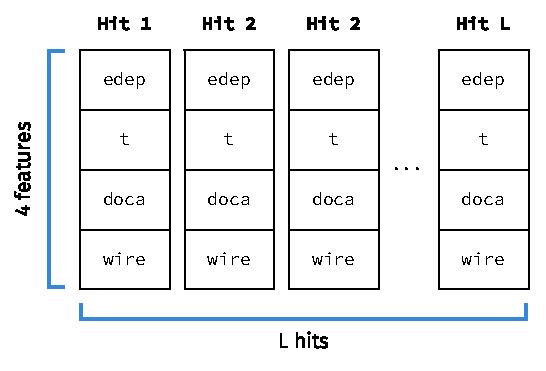
\includegraphics[width=0.5\textwidth]{chapter4/hit_sequence.drawio.pdf}
    \caption{Structure of one training sample. Hits are arranged into
    fixed-length sequences in the {\sc Geant4} order, i.e.\ whereby hits from
    the same track are contiguous.}
    \label{fig:hit_data_structure}
\end{figure}


%In COMET Phase-I, events of particular interest come in the form of extended
% tracks in the CDC, whose accurate reconstruction (in both momentum and
% position) is paramount to the identification of a conversion signal. These
% tracks typically produce hits in very specific patterns, dictated by the
% particle's exact trajectory and energy loss in the gas. We expect a
% data-driven generative model to struggle in replicating the exact signature of
% such tracks, hence we decided early on to restrict the scope of the model to
% events that lack any physics-rich features. ^ not necessarily true. it's not
% only for that reason, but also because we want fine control over the rates of
% specific events (e.g. signal-like)

\subsection{Event selection}

% Consequences: we have to combine MC and GAN data ---> means we have to find a
% way to produce MC selectively ---> and then mix hits in the right proportions
% to get mock data.

Not all MC events are fed to the GAN for training. In particular, potential
background sources, i.e.\ particles with a momentum around
\SI{105}{MeV/\clight}, produce characteristic series of hits in the CDC which
are likely to be reconstructed by a track fitting algorithm. Such a particle's
trajectory is firmly dictated by the Lorentz force, which is a constraint
difficult to impose on a GAN model. In addition, a GAN might generate too large
or too small a proportion of reconstructible events, leading to more uncertainty
in the background rates estimated from samples containing synthetic hits. Unlike
MC data, fake tracks can yield no information concerning their origin, as the
GAN-generated hits come completely unlabelled.

These reasons motivate a splitting of the dataset into \emph{reconstructible}
events, which only the MC simulation may simulate, and \emph{noise-like} events,
where no reconstructible track occurs, and the data is deemed ``uninteresting''
enough that it can be augmented by the GAN without biasing the physical results.

% EVENT RECOMBINATION Once the GAN model is trained, it should be able to
%efficiently generate noise-like hits which must then be mixed back into
%MC-simulated reconstructible events in the right proportions. Because the
%generative neural network can leverage parallel processing and GPUs, noise-like
%data is expected to be cheap to produce, hence the bottleneck remains with the
%MC simulation. However the yield of reconstructible events may be increased
%with selective event sampling. 

In each MC event (corresponding to the outcomes of one proton-on-target
collision), we determine if at least one particle with $p >
\SI{50}{\MeV/\clight}$ has entered the CDC and produced at least 4 hits. In this
case, all hits from the event are given the ``reconstructible'' label and will
not be used to train the GAN. If no reconstructible track has occurred during
the event, all hits are considered noise-like and are added to the training
dataset. Figure~\ref{fig:cdc_rconst_vs_noise} compares noise-like and
reconstructible hits and outlines the difference in structure between the two
categories.

\begin{figure}
    \centering
    %\captionsetup[subfigure]{justification=centering}
    \begin{subfigure}[t]{0.45\textwidth}
        \centering
        \hspace{-1cm} % To align graphics with caption
        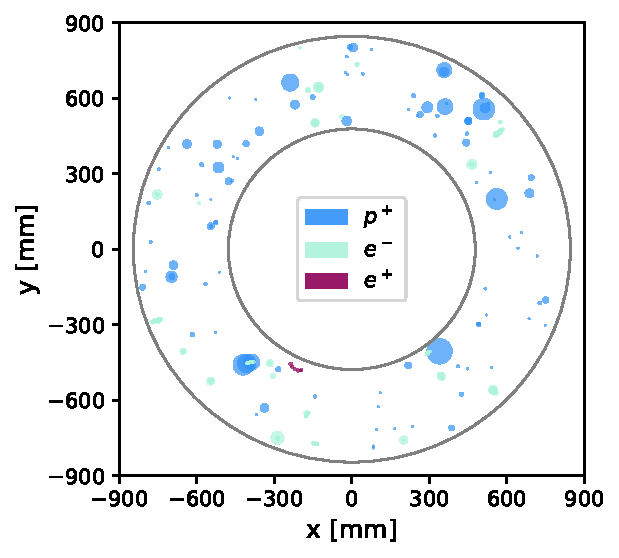
\includegraphics[width=\textwidth]{chapter4/only_noiselike_events.pdf}
        \caption{Noise-like hits from 100 MC events.}
        \label{fig:cdc_rconst_vs_noise:low}
    \end{subfigure}
    \begin{subfigure}[t]{0.45\textwidth}
        \centering
        \hspace{-1cm} % To align graphics with caption
        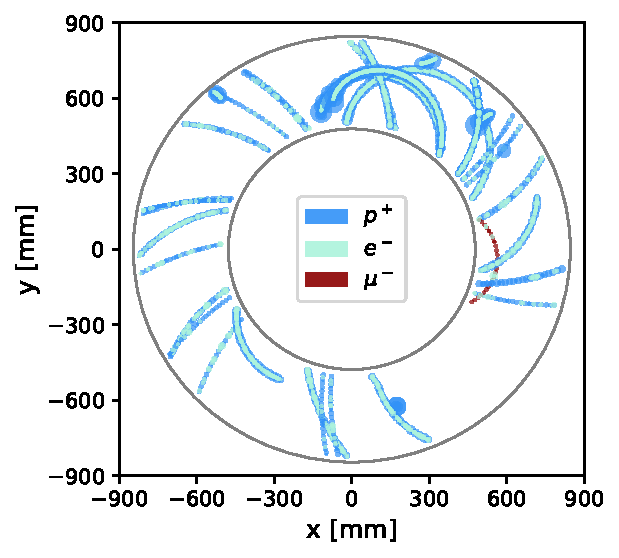
\includegraphics[width=\textwidth]{chapter4/only_reconstructible_events.pdf}
        \caption{Reconstructible hits from 10 MC events.}
        \label{fig:cdc_rconst_vs_noise:high}
    \end{subfigure}
    \caption{Comparison of hit patterns in the CDC depending on whether or not a reconstructible track occurred. The area of each hit is proportional to the amount of energy deposited, and the colour denotes particle type.}
    \label{fig:cdc_rconst_vs_noise}
\end{figure}

The MC5 dataset contains $10^{9}$ events of which \numprint{51137} have hits in
the CDC. Of those, \numprint{2036} events have at least one reconstructible track, and
\numprint{49101} events do not. Inside this latter category, \numprint{634266} hits are
present, and these make up the GAN training dataset.

% MC5A02 calculation of noise-like vs reconstructible events/hits: Total events:
% 990678399 Hit classification: 2036 unique events (rate 2e-6) with
% reconstructible hits (63648 hits) 49101 unique events (rate 5e-5) with
% noiselike hits (634266 hits)



%In order to preserve the information present in events where signal-like tracks
%occur,  MC events are split into two categories, depending on whether or not at
%least one \emph{reconstructible} track appeared in the CDC during the event.
%The GAN is only trained on noise-like hits, while simulating reconstructible
%events is reserved to the Monte Carlo simulation, such that all reconstructed
%tracks have a history which can be retraced all the way to the proton
%collision. This effectively prevents the GAN from producing fake signal-like
%tracks unconstrained, which could cause excessive uncertainties in the
%estimated background rates. However, the two categories of events must now be
%produced separately and later recombined in the right proportions, which adds
%some complexity to the task.

%Training the GAN to generate individual hits is sufficient to model the
%underlying distributions of the four features, but the generated hits lack
%coherence. In the training dataset, when multiple hits are produced by a single
%track, they often occur next to each other in time and space. The GAN model
%must be allowed to see and process the relationship between consecutive hits
%for the generated hits to resemble simulated ones. Hence instead of having the
%model process single hits, it makes sense to feed it sequences of consecutive
%hits such that temporal information can be processed as well. The architecture
%of $G$ and $D$ should be allowed to accommodate for this extra dimension.


% This is what hits from p>50MeV tracks look like, and this is what hits from
% p<50MeV tracks look like. From the observation that the former tends to have
% reconstructible hit patterns while the latter contains single hits and
% localised patterns, we categorise MC events according to whether they contain
% a p>50MeV track or not. We then use hits from non-reconstructible events as
% the training data for our generative model whose goal is to learn the patterns
% and generate original samples of hits that we can use as a background onto
% which we will overlay reconstructible MC-simulated events. The result is the
% offloading of 99% of the simulation to the generative model which is highly
% efficient. 



\subsection{Pre-processing}
The three continuous hit features (energy deposit, time and DCA) are physical
quantities with different units and scales. Their distributions are shown in
Figure~\ref{fig:original_feature_distributions}. In order to maximise gradient
flow in the discriminator, it is common practice for all features to be
re-scaled into a fixed range, e.g.\ $[0, 1]$. However, in the case of highly
uneven and/or discontinuous distributions, the generator can struggle to model
the data which results in a distribution of generated data which does not match
the distribution of training data.

\begin{figure}
    \centering
    \noindent\makebox[\linewidth][c]{
        \begin{subfigure}[t]{0.35\textwidth}
            \centering
            \hspace{-0.5cm}
            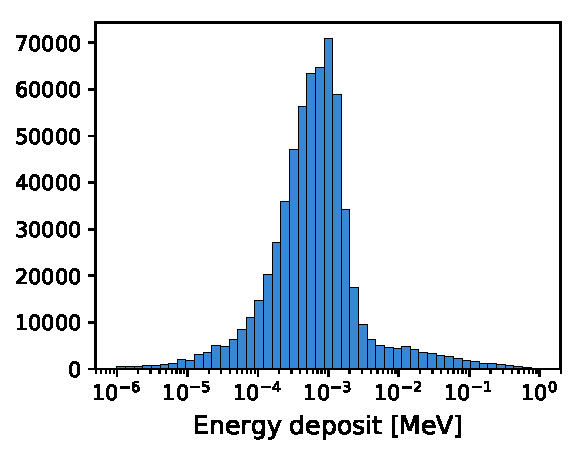
\includegraphics[width=\textwidth]{chapter4/real_edep.pdf}
            %\caption{}
        \end{subfigure}
        \begin{subfigure}[t]{0.35\textwidth}
            \centering
            \hspace{-0.5cm}
            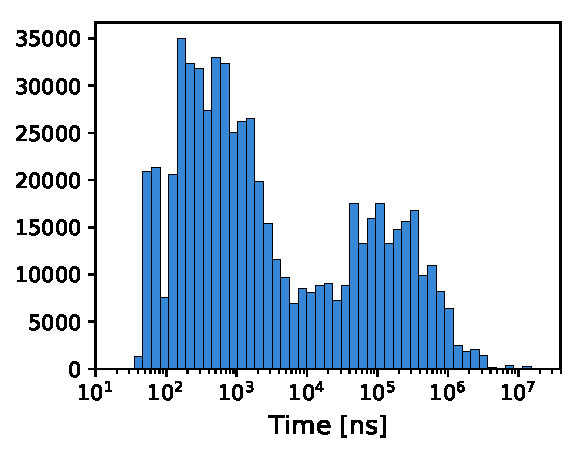
\includegraphics[width=\textwidth]{chapter4/real_t.pdf}
            %\caption{}
        \end{subfigure}
        \begin{subfigure}[t]{0.35\textwidth}
            \centering
            \hspace{-0.5cm}
            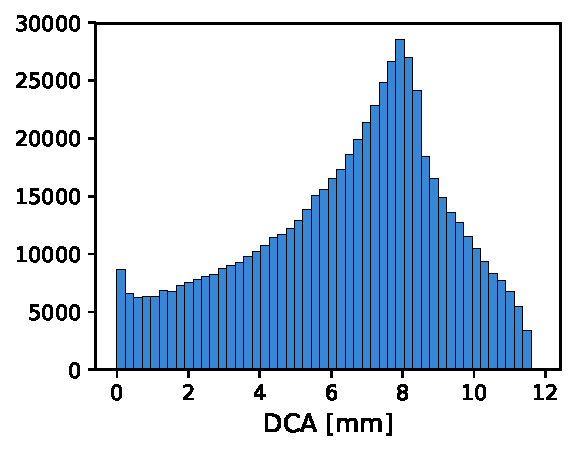
\includegraphics[width=\textwidth]{chapter4/real_doca.pdf}
            %\caption{}
        \end{subfigure}}
    \caption{Distributions of the three continuous features used to train the GAN.}
    \label{fig:original_feature_distributions}
\end{figure}

To alleviate this issue and define a common scale for all continuous features,
each feature undergoes a non-linear \emph{quantile transformation}, which
corresponds to a mapping from each value $x_i$ to $y_i = \Phi^{-1}(F(x_i))$,
where $F$ is the empirical cumulative distribution function (CDF) of the
feature, and $\Phi$ is the Gaussian CDF. This transformation effectively yields
normally distributed features, which the generator can more easily reproduce.
Its task is not however made trivial, as the correlations between features
remain, which it must learn to model.

In addition to the quantile transformation, the values of each feature are
re-scaled independently to lie within the $[-1, 1]$ range. To prevent the
generator from producing values out of this range, which would give the
discriminator a clear indication of a sample being fake, the hyperbolic tangent
function is used as the generator's final layer.

%We use the standard classes \texttt{preprocessing.QuantileTransformer} and
%\texttt{preprocessing.MinMaxScaler} from the Scikit-learn~\cite{sklearn}
%package to apply these pre-processing steps.

%The fourth feature, wire index, is not modified prior to training. However, as
% the only discrete quantity, it receives a special treatment by the networks
% during training. More? Less?

\subsection{Hit sequence sampling and data augmentation}
At each step of the training, the discriminator receives two mini-batches of hit
sequences: one from the training data and one synthesised by the generator. The
discriminator's output is then used to compute the loss for $G$ and $D$,
according to Equations~\ref{eq:WGAN-GP} and~\ref{eq:WGAN-GP_gen}.

To allow parallel processing of the hit sequences by the networks, a fixed
sequence length $L$ is defined prior to training. Hence hits can be packed
into dense tensors upon which vectorised operations can be applied. Typically, a
sequence will contain concatenated sets of hits from multiple tracks and from
multiple events.

Hits belonging to different events are completely unrelated, as they are not the
product of the same POT collision. This provides freedom to swap events and
concatenate their hits in any order. The order of hits within the same event
should however be preserved. 
Combining events in many different ways enhances the diversity and size of the
training dataset, which alleviates the possibility of overfit or mode collapse.
Concatenating the \numprint{634266} hits linearly into sequences of length
$L=512$ would yield only 1239 samples. By rearranging the events, we produce
\numprint{500000} unique samples which the GAN learns from. Although it is not
the maximum number of event re-combinations, this number of samples was found to
be large enough to prevent overfit of our GAN model.


\subsection{Network components}

\subsubsection{Temporal convolutions}
In order to process sequences of hits efficiently, both networks use a series of
convolutional layers which --- unintuitively --- apply cross-correlation
operations between the input $x$ and the learned kernel $w$:
\begin{equation}\label{eq:conv1d}
    %y_{i} = (x \ast w)_{i} + b = \sum_{j=1}^{C_\mathrm{in}} \sum_{k=-(K-1)/2}^{(K-1)/2} w_k\ x_{i+k,j} + b,
    y_{i} = (w \ast x)_{i} = \sum_{k} w_k \cdot x_{i+k},
\end{equation}
where $i$ is the position along the output sequence $y$, and $k$ runs over the
kernel weights. This operation is illustrated in Figure~\ref{fig:temporal_conv}.

\begin{figure}
    \centering
    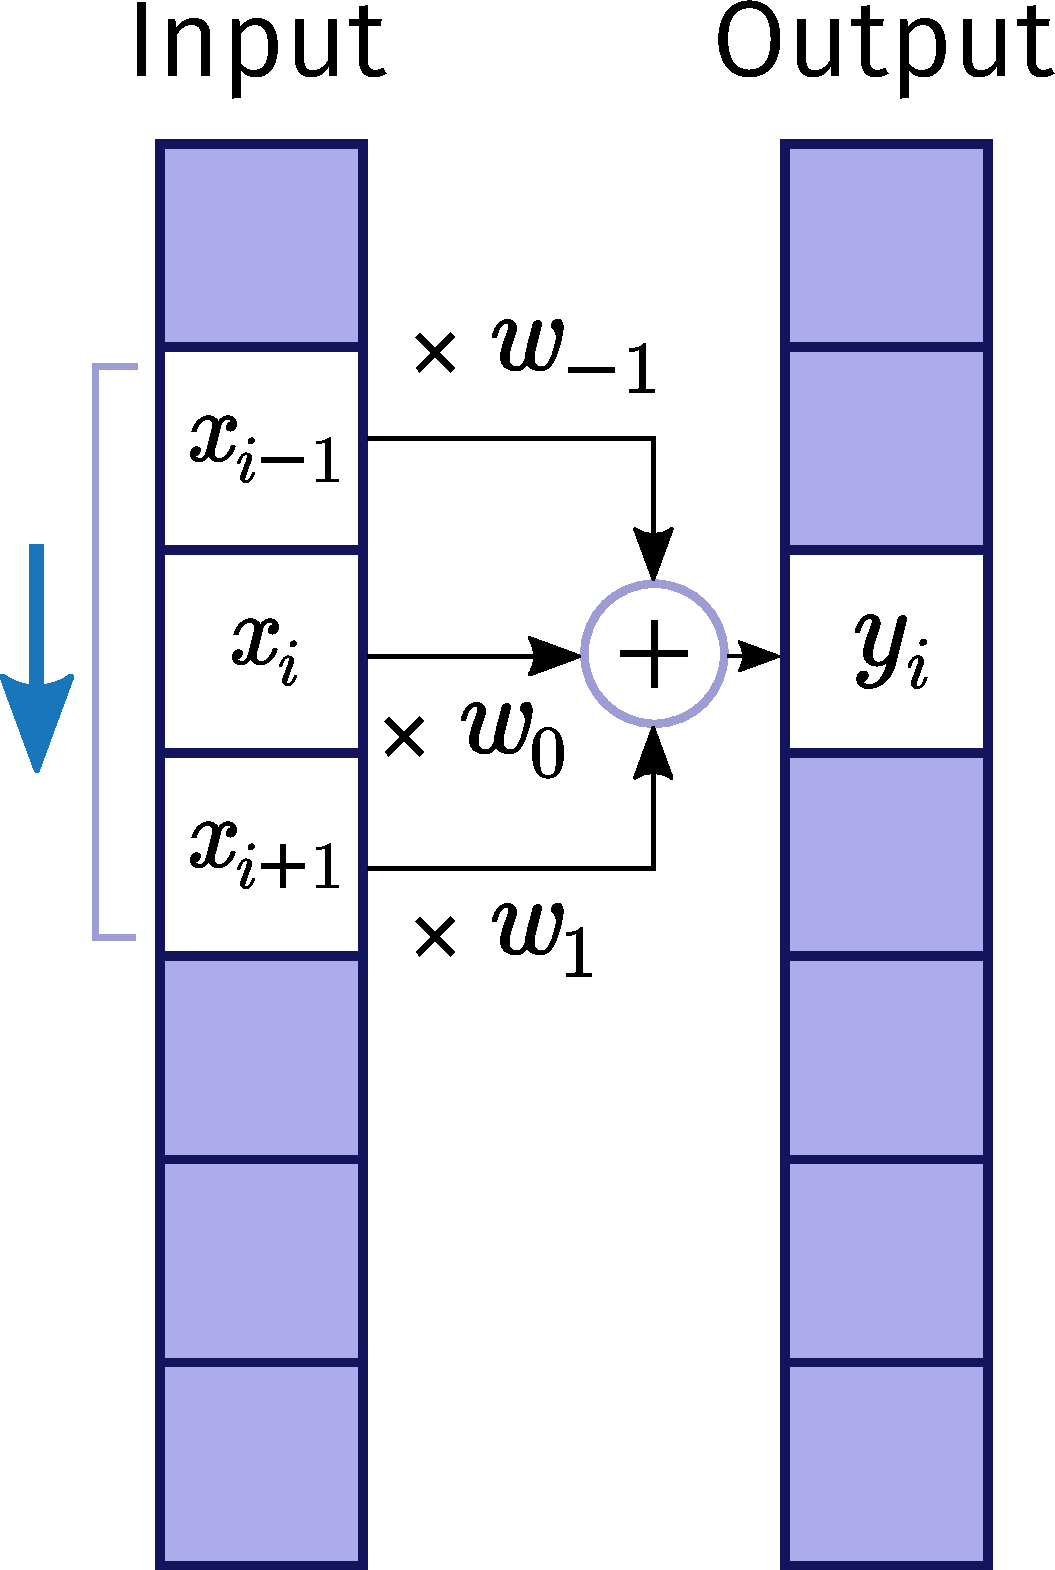
\includegraphics[width=0.20\textwidth]{chapter4/1d_convolution.pdf}
    \caption{Temporal (1D) convolution operation with kernel size 3. For
    clarity, both the input and output sequences have one channel, i.e.\
    $C_\mathrm{in} = C_\mathrm{out} = 1$. The blue arrow shows the direction along
    which the kernel slides across the input sequence.}
    \label{fig:temporal_conv}
\end{figure}


Unlike in the common case of raster images, the input to the discriminator is
not a two-dimensional array of pixels, but a one-dimensional sequence of hits.
Hence, the kernels are also one dimensional. The ``channels'' of the input
sequence correspond to features of the hits. Within a convolutional layer,
Equation~\ref{eq:conv1d} is applied as many times as there are channels in the input
sequence, and the result is the sum over channels. The operation can also be
applied in parallel with many different kernels, in which case each kernel will
produce one channel in the output sequence.


The fact that the kernel acts on adjacent elements implies that the network
effectively processes multiple consecutive hits at a time. This allows the
generator to synthesise coherent sequences and the discriminator to perceive
whether a generated sequence has the same overarching structure as real
sequences.

%\subsubsection{Strided convolutions for up- and down-sampling}
Optionally, convolution kernels can be applied over the sequence with a stride,
meaning that the kernel moves down by more than one element between two
cross-correlation operations. This has the effect of producing an output
sequence that is shorter than the input sequence. This is often used to allow
the network to see the data over increasingly large scales and to keep the total
number of operations reasonable in layers where the input has many channels.

%In the generator, fractionally-strided convolutions are used in order for the
%sequence length to increase


%The discriminator takes as input a sequence of hits of length $L$. Each hit is
%described by four features: energy deposit, time, distance of closest approach
%and wire index. The first convolutional layer computes feature maps by sliding
%its kernels over the hit sequence. A non-linear activation function is applied
%to the feature maps before passing them on to the next layer. In our case, the
%leaky rectified linear unit, or
%\texttt{LeakyReLU}~\cite{Maas13rectifiernonlinearities}, is used as the
%non-linearity. ^ Too much detail?


\subsubsection{Residual connections}
\begin{figure}
    \centering
    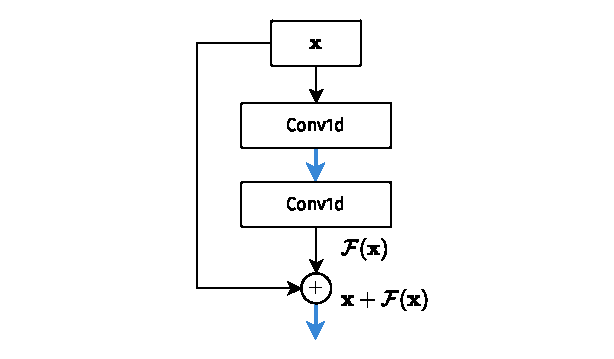
\includegraphics[width=0.6\textwidth]{chapter4/residual_sel.drawio.pdf}
    \caption{Residual blocks used in both networks to facilitate gradient flow.
    Blue arrows indicate an activation function.}
    \label{fig:residual_block}
\end{figure}
In order to facilitate gradient flow from the discriminator to the generator and
thus speed up training, convolutional layers can be replaced by residual
blocks~\cite{he2016deep} in both networks. A residual block combines two
convolutional layers with a residual connection from the input to the output,
allowing the gradients to propagate via two paths, as shown in
Figure~\ref{fig:residual_block}. The output $\bm{y}$ of the block can be
written as
%\begin{equation*}
    $\bm{y} = \mathcal{F}(\bm{x}) + \bm{x},$
    %\bm{y} = \mathcal{F}(\bm{x}) + W_s \bm{x},
%\end{equation*}
where $\mathcal{F}$ represents the operation of the two convolutional layers and
$\bm{x}$ is the input tensor. 
When $\mathcal{F}(\bm{x})$ and $\bm{x}$ have different shapes, a
dimension-matching linear transformation can be applied to $\bm{x}$. In this
case, the result is $\bm{y} = \mathcal{F}(\bm{x}) + W \bm{x}$, where the
weights of the $W$ tensor are adjusted during training.


\subsection{Network architectures}
Having introduced the building blocks, we can now assemble them into our
discriminator and generator. The two networks, shown schematically in
Figure~\ref{fig:architectures}, are composed of stacked residual blocks, which
progressively increase the size of the sequence in the generator, or decrease it
in the discriminator.

\begin{figure}
    \centering
    \begin{subfigure}[t]{0.49\textwidth}
        \centering
        \caption{Generator.}
        \vspace{0.3cm}
        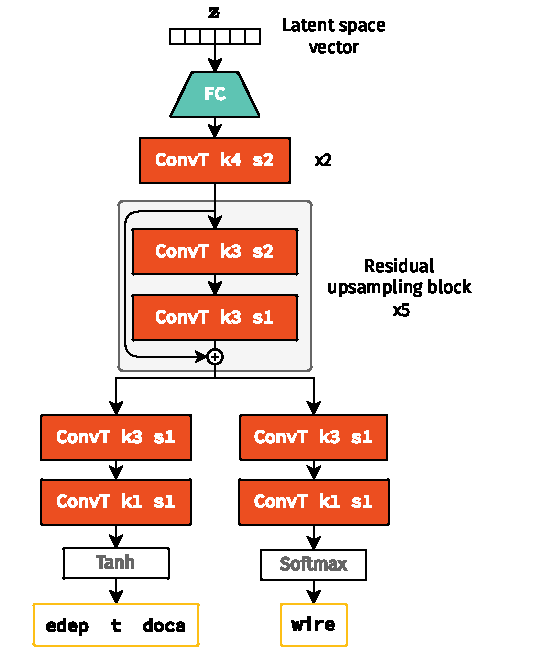
\includegraphics[width=\textwidth]{chapter4/network_architectures_gen.drawio.pdf}
        \hspace{-1cm} % To align graphics with caption
    \end{subfigure}
    \\
    \vspace{0.5cm}
    \begin{subfigure}[t]{0.49\textwidth}
        \centering
        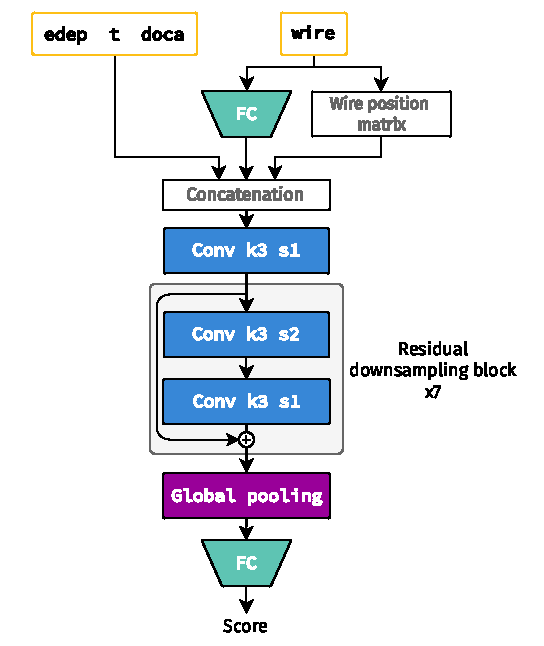
\includegraphics[width=\textwidth]{chapter4/network_architectures_disc.drawio.pdf}
        \hspace{-1cm} % To align graphics with caption
        \caption{Discriminator.}
    \end{subfigure}
    \caption{Network architectures. The layer types are: \texttt{FC} for
        fully-connected, \texttt{Conv} for a standard convolution and
        \texttt{ConvT} for a transposed (fractionally-strided) convolution. In
        convolutional layers, kernel size and stride are denoted by \texttt{k}
        and \texttt{s}, respectively.}
    \label{fig:architectures}
\end{figure}

\subsubsection{Data flow}
In the generator, the input vector, sampled from latent space, is first passed
through a fully-connected layer, after which it is reshaped to have a length of
4. The proto-sequence is then up-sampled by fractionally-strided convolutional
layers, adding finer and finer details to the sample. As the length increases,
the number of channels is decreased to limit the total number of operations and
the network's complexity. Once the sample has reached a length of $L$, the
information is projected to data space: to obtain the continuous features, a
convolutional layer with three output channels is applied and its output passed
through a $\tanh$ function, yielding values in the range $[-1, 1]$; while for
the discrete wire index, we use a layer with 4986 output channels\footnote{As
many as there are wires.} followed by a softmax\footnote{Defined as
$\mathrm{Softmax}(\bm{x})_i = \frac{\exp(-x_i)}{\sum_j \exp(-x_j)}.$}
function to determine the network's preferred choice of wire for each hit.

The discriminator extracts information from the input hits through its
convolutional layers, progressively down-sampling the sequence while increasing
the number of channels. After 7 residual blocks, a global average pooling is
performed, i.e.\ for each channel, the result is the average value over the
sequence. The resulting tensor is passed through a final fully-connected layer,
combining the features into a single scalar which is the score for that sample.

\subsubsection{Gradient flow for discrete features}
We would like for the discriminator to have some knowledge of where, in the
detector, hits are located, so that it can use this knowledge as a criterion in
its judgement. A straightforward way to give this information to the
discriminator would be to use the wire index to query a lookup table of wire
positions. However, indexing an array is not a differentiable operation, hence
it does not allow gradients to flow from the output score to the generator
weights, and this prevents the generator from learning to accurately position
hits.

To allow gradient flow, we can represent the wire index as a \emph{one-hot
encoded} vector, whose size is the total number of wires, and where only the
entry corresponding to the index is 1, and the others are 0. This vector
representation can be used in differentiable operations to query a particular
entry in a table: if we represent the table of wire positions as a matrix $W$
with dimensions $2 \times 4986$, and the one-hot encoded wire vector as a
4986-dimensional vector $\bm{v}$, the product $W \cdot \bm{v}$ is a
differentiable operation and its output is the wire's position since the one-hot
vector picks out the correct entry from the position matrix.

In the case of generated hits, the wire vector is not exactly one-hot: instead,
the output of the softmax operation is a vector of real-valued probabilities for
each wire. The multiplication of the above wire position matrix with such a
vector can be interpreted as a weighted sum of all wire positions with the
weight corresponding to the softmax probability. Hence, the result is not an
exact wire location but an approximate region of the detector in which the
generator envisions the hit to be.

As discussed in Reference~\cite{NIPS2017_892c3b1c}, one might suspect that the
discriminator can learn to reject the output of the generator because it does
not look like a one-hot vector. However, the Wasserstein distance between the
real and generated data remains well-defined and continuous even in this
particular case of a discrete variable, hence using the WGAN loss does allow the
networks to learn.


\subsection{Training}
The networks are trained via gradient descent of the WGAN-GP loss, using the
Adam~\cite{Kingma2015AdamAM} algorithm. The PyTorch framework with which the GAN
is implemented allows all tensor operations to be performed on an Nvidia Graphics
Processing Unit (GPU) via CUDA, which speeds up training iterations roughly
tenfold. Hyperparameters, such as learning rate and $\lambda_{GP}$, were
initially set to a default value from common practice guidelines and then
adjusted if needed to ensure stable loss curves.
Table~\ref{tab:training_hyperparameters} summarises the values of various
hyperparameters, and Figure~\ref{fig:gan_losses} shows the loss curves for $G$
and $D$ over 200 training epochs.

\begin{table}[]
    \centering
    \begin{tabular}{cccccc}
        \toprule
        Optimiser & Learning rate & $(\beta_1, \beta_2)$ & Sequence length & Loss &
        $\lambda_\mathrm{GP}$
        \\\midrule 
        Adam & $10^{-4}$ & $(0.9, 0.999)$ & 512 & WGAN-GP & 10
        \\\bottomrule
    \end{tabular}
    \caption{Training hyperparameters.}
    \label{tab:training_hyperparameters}
\end{table}

The loss functions for $D$ and $G$ evaluated at each training step are recorded
to show the progression and ensure that the networks are learning. In addition,
every 100 mini-batch iterations, the critic loss is evaluated on test samples
which are absent from the training dataset. This allows us to determine whether
$D$ is overfitting to the training data, in which case the loss calculated using
training and test samples (Figure~\ref{fig:gan_losses:test}) would diverge, as
demonstrated in Reference~\cite{NIPS2017_892c3b1c}.


\begin{figure}
    \centering
    \begin{subfigure}{0.49\textwidth}
        \centering
        \hspace{-1cm} % alignment
        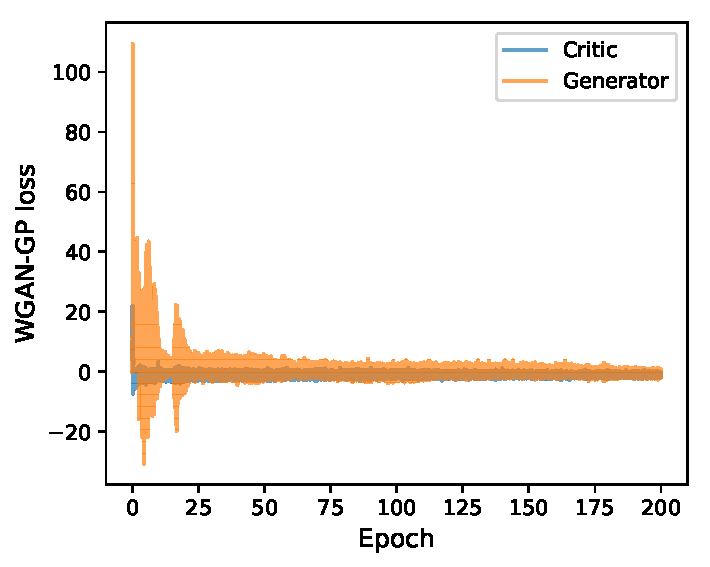
\includegraphics[width=0.95\textwidth]{chapter4/losses.pdf}
        \caption{Critic and generator losses.}
    \end{subfigure}
    \hfill
    \begin{subfigure}{0.49\textwidth}
        \centering
        \hspace{-1cm} % alignment
        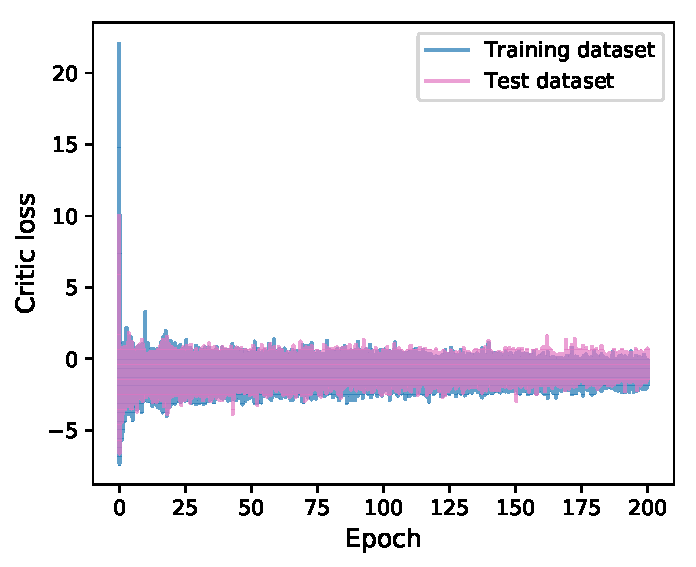
\includegraphics[width=0.95\textwidth]{chapter4/val_loss.pdf}
        \caption{Critic loss for training and test samples.}
        \label{fig:gan_losses:test}
    \end{subfigure}
    \caption{Loss curves as a function of training epochs.}
    \label{fig:gan_losses}
\end{figure}

% Weight initialisation def weight_init_gen(m): classname = m.__class__.__name__
% if classname.find('Conv') != -1: nn.init.normal_(m.weight, 0.0, 0.02) if
% m.bias is not None: nn.init.zeros_(m.bias)

% def weight_init_disc(m): classname = m.__class__.__name__ if
%     classname.find('Conv') != -1: nn.init.normal_(m.weight, 0.0, 0.02) if
%     m.bias is not None: nn.init.zeros_(m.bias) if classname.find('Linear') !=
%     -1: nn.init.normal_(m.weight, 0.0, 0.02) if m.bias is not None:
%     nn.init.zeros_(m.bias)



\subsection{Evaluation}
\label{sec:gan_eval}
Evaluation of GAN-generated samples is notoriously difficult in all domains
because of the lack of a well-defined, unique metric for quality\footnote{Unlike
in supervised learning, where an obvious quality metric is usually the loss
function itself.}. The score
returned by the discriminator network is dependent upon its exact architecture,
the dataset and all hyperparameters, hence it cannot be used as a reliable metric. 

Unlike natural images which can be examined visually to determine whether
they depict something real, sequences of hits in a detector are difficult to
evaluate perceptually. 
Figure~\ref{fig:comp_uncurated} shows a comparison between uncurated individual
samples, four from the training dataset and four generated by $G$. In this type
of evaluation, we try to exacerbate any differences in the features and
sequence structure through colours and visual hints such as lines connecting
consecutive hits.

On a larger scale, we also compare the distributions of hit features across many
samples in order to verify that the GAN can model the dataset properly. Drawing
2D histograms of each pair of features, as in
Figure~\ref{fig:comp_feature_distributions}, also reveals whether feature
correlations are faithfully modelled by $G$.

\begin{figure}
    \centering
    %\captionsetup[subfigure]{justification=centering}
    \begin{subfigure}[t]{0.48\textwidth}
        \centering
        \hspace{-1cm} % To align graphics with caption
        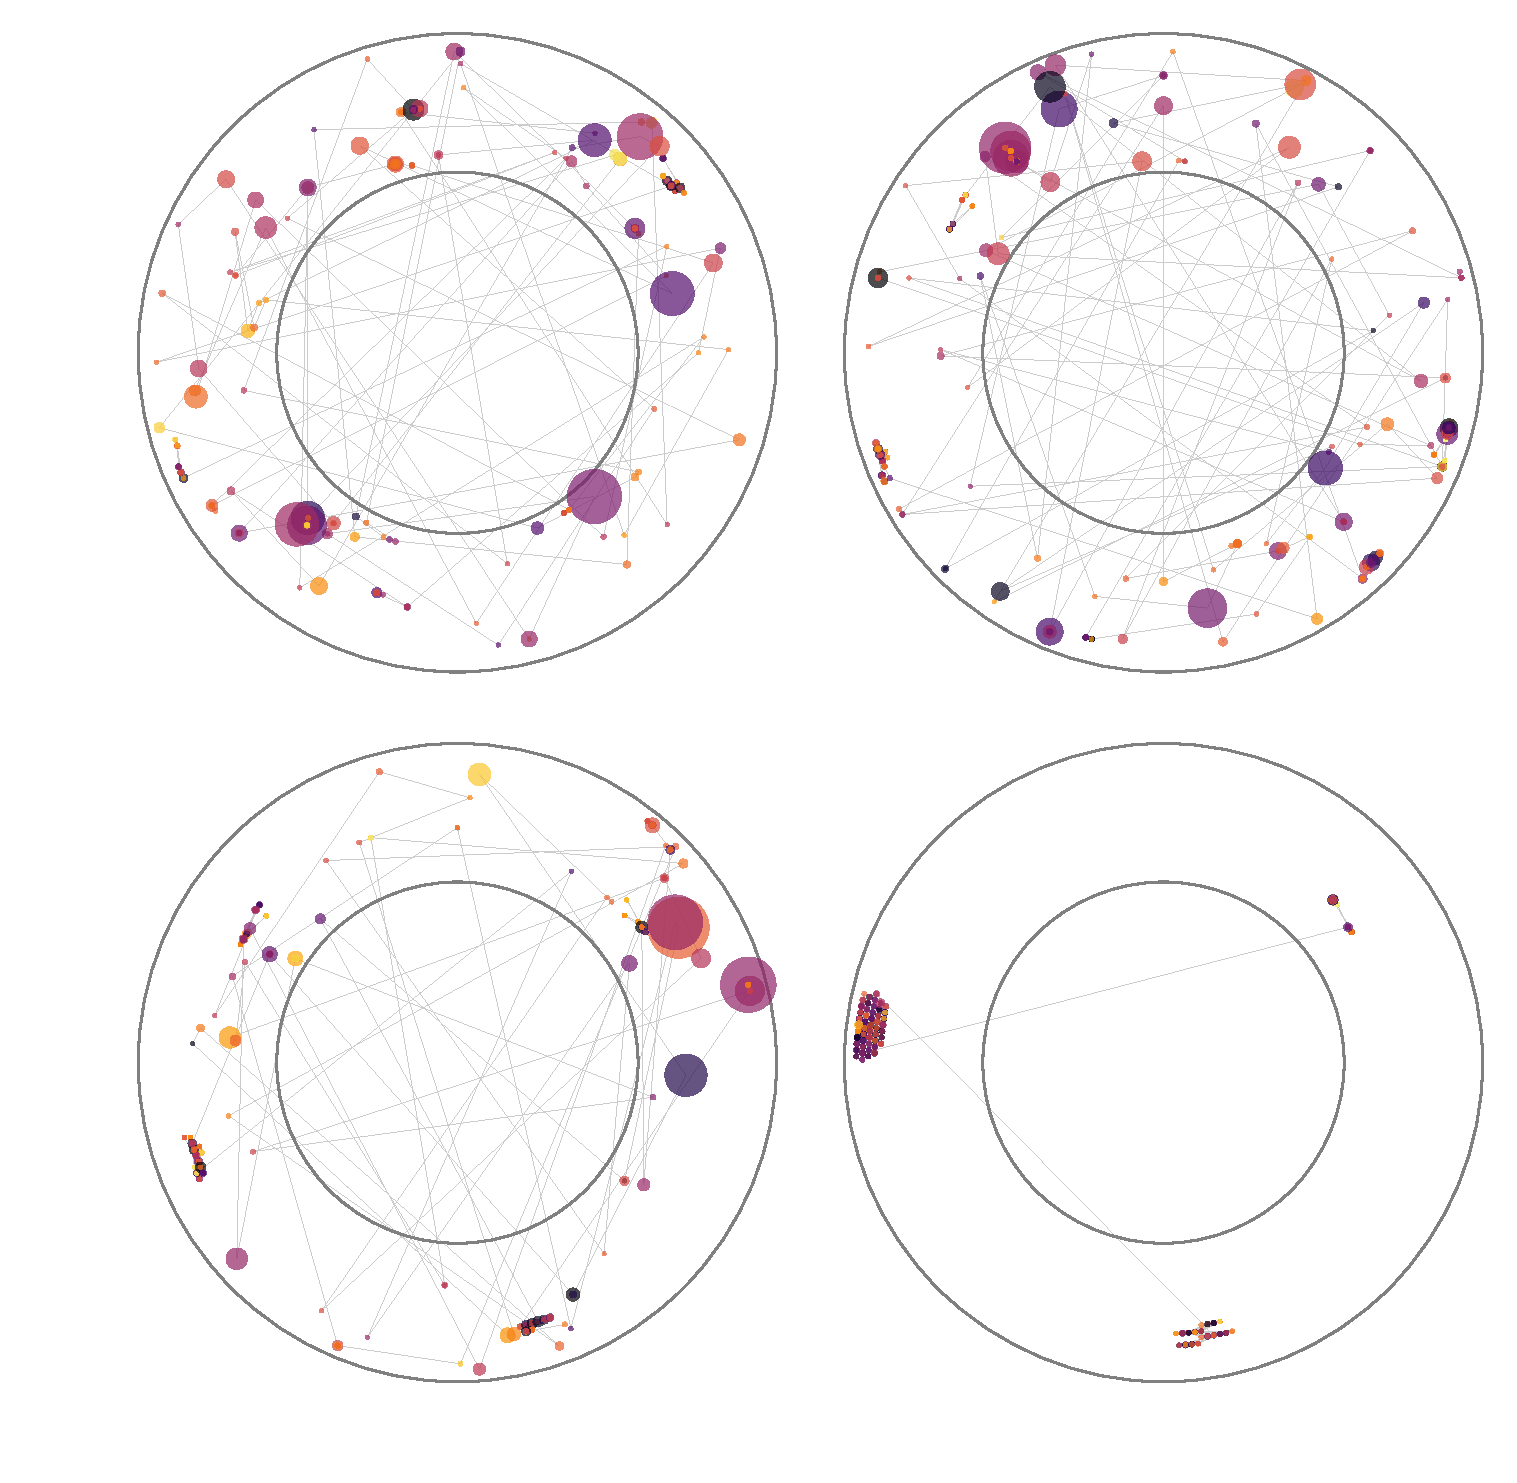
\includegraphics[width=\textwidth]{chapter4/grid_real_4.pdf}
        \caption{Training samples.}
    \end{subfigure}
    \quad
    \begin{subfigure}[t]{0.48\textwidth}
        \centering
        \hspace{-1cm} % To align graphics with caption
        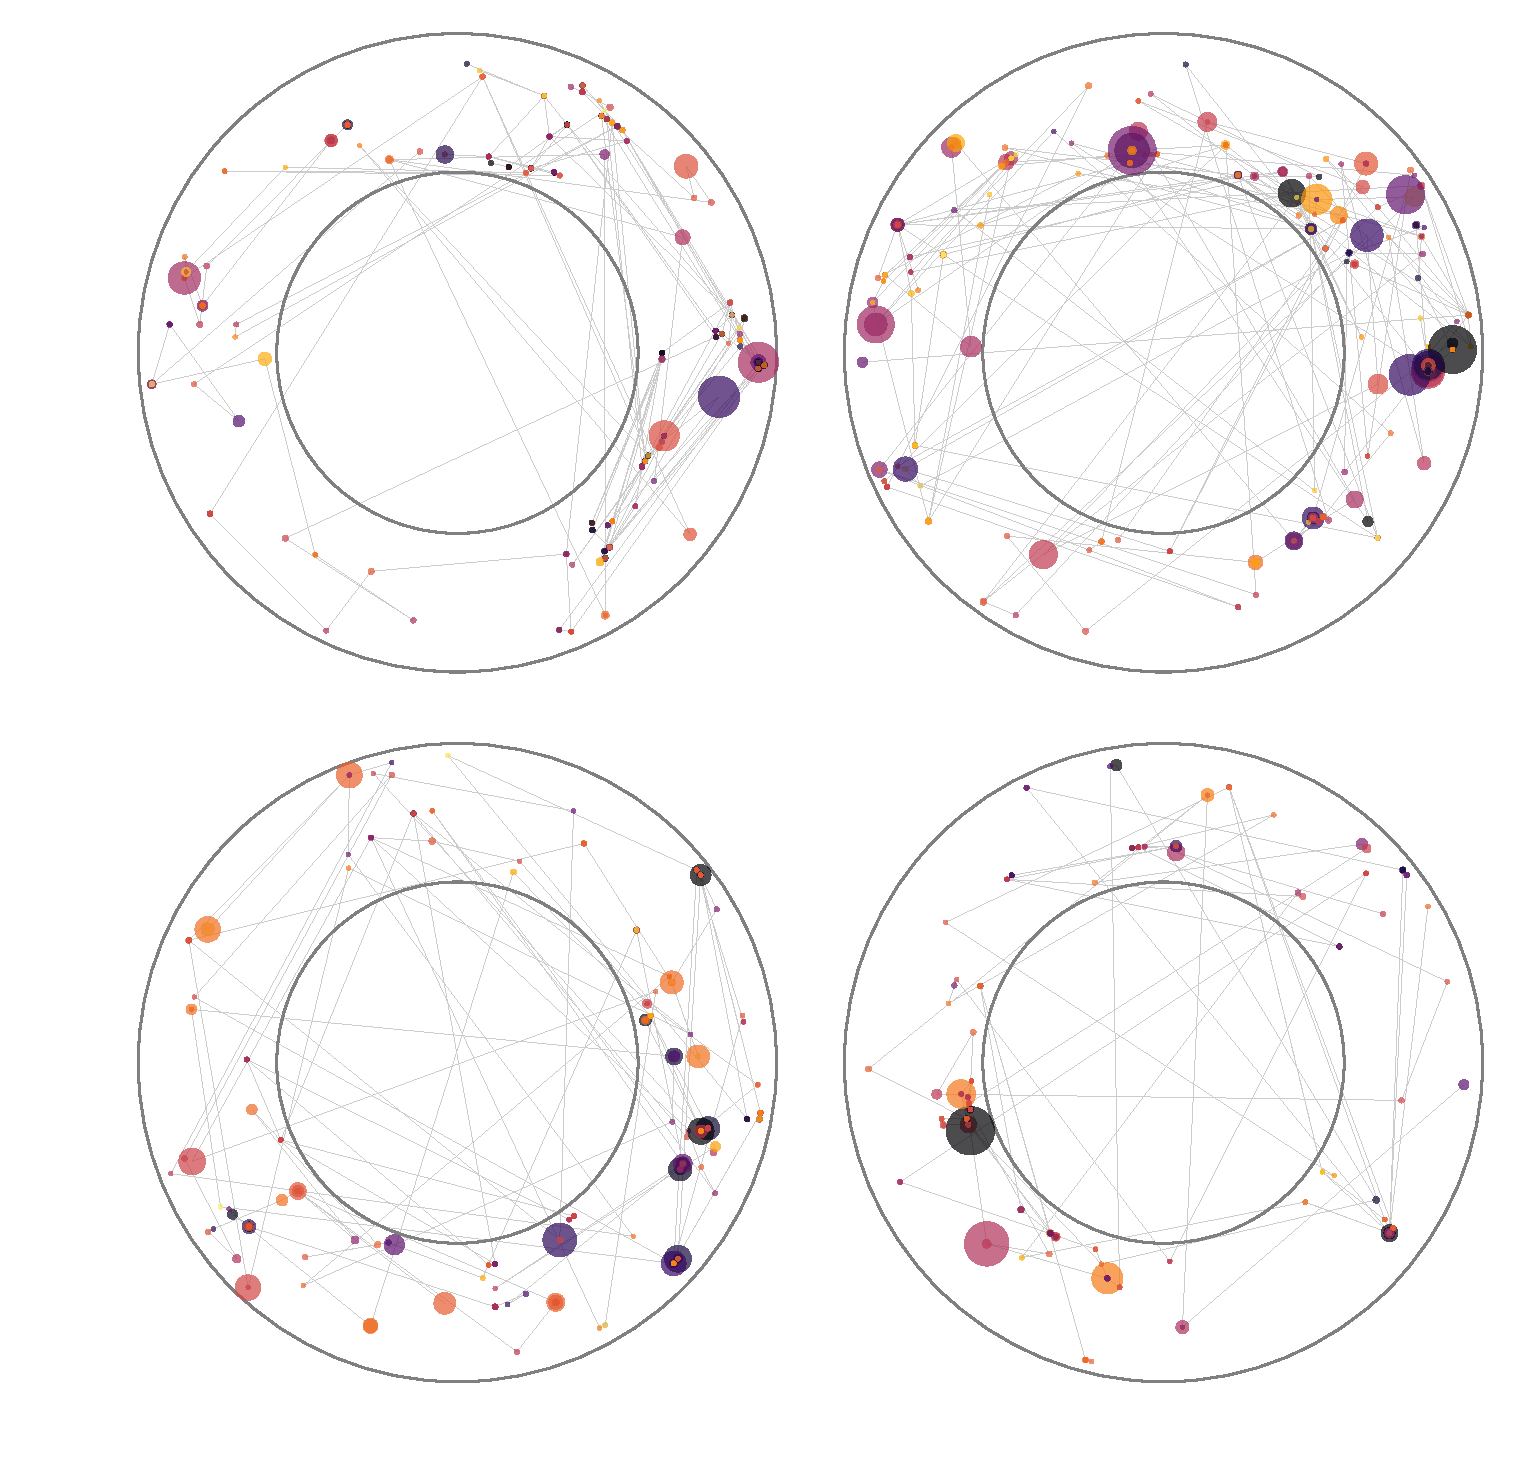
\includegraphics[width=\textwidth]{chapter4/grid_fake_4.pdf}
        \caption{Generated samples.}
    \end{subfigure}
    \caption{
        Comparison of individual samples, comprised of 512 hits. Hits are
        represented by a circle whose area is proportional to the energy deposit
        and whose colour shows distance of closest approach. 
        Lines connect consecutive hits in the sequence.
        %Only three features out of four can be examined and compared using
        %these plots unless we add an extra dimension.
    }
    \label{fig:comp_uncurated}
\end{figure}

\begin{figure}
    \centering
    %\captionsetup[subfigure]{justification=centering}
    \begin{subfigure}[t]{0.48\textwidth}
        \centering
        \hspace{-1cm} % To align graphics with caption
        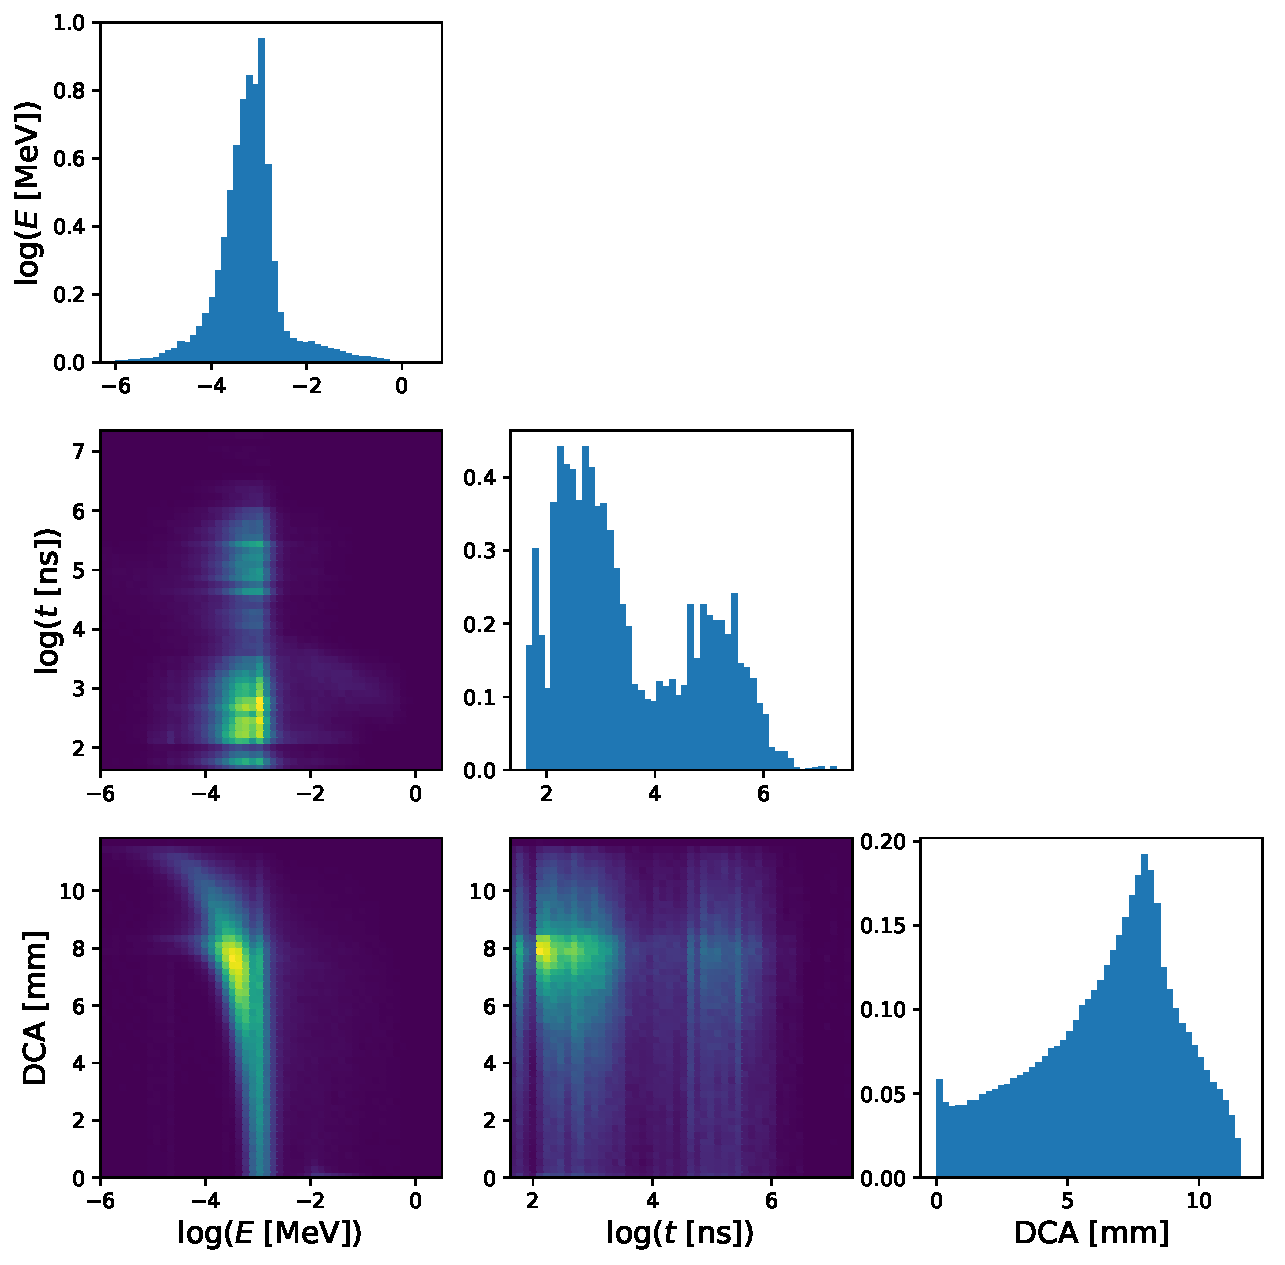
\includegraphics[width=\textwidth]{chapter4/feature_matrix_real.pdf}
        \caption{Training dataset.}
    \end{subfigure}
    \quad
    \begin{subfigure}[t]{0.48\textwidth}
        \centering
        \hspace{-1cm} % To align graphics with caption
        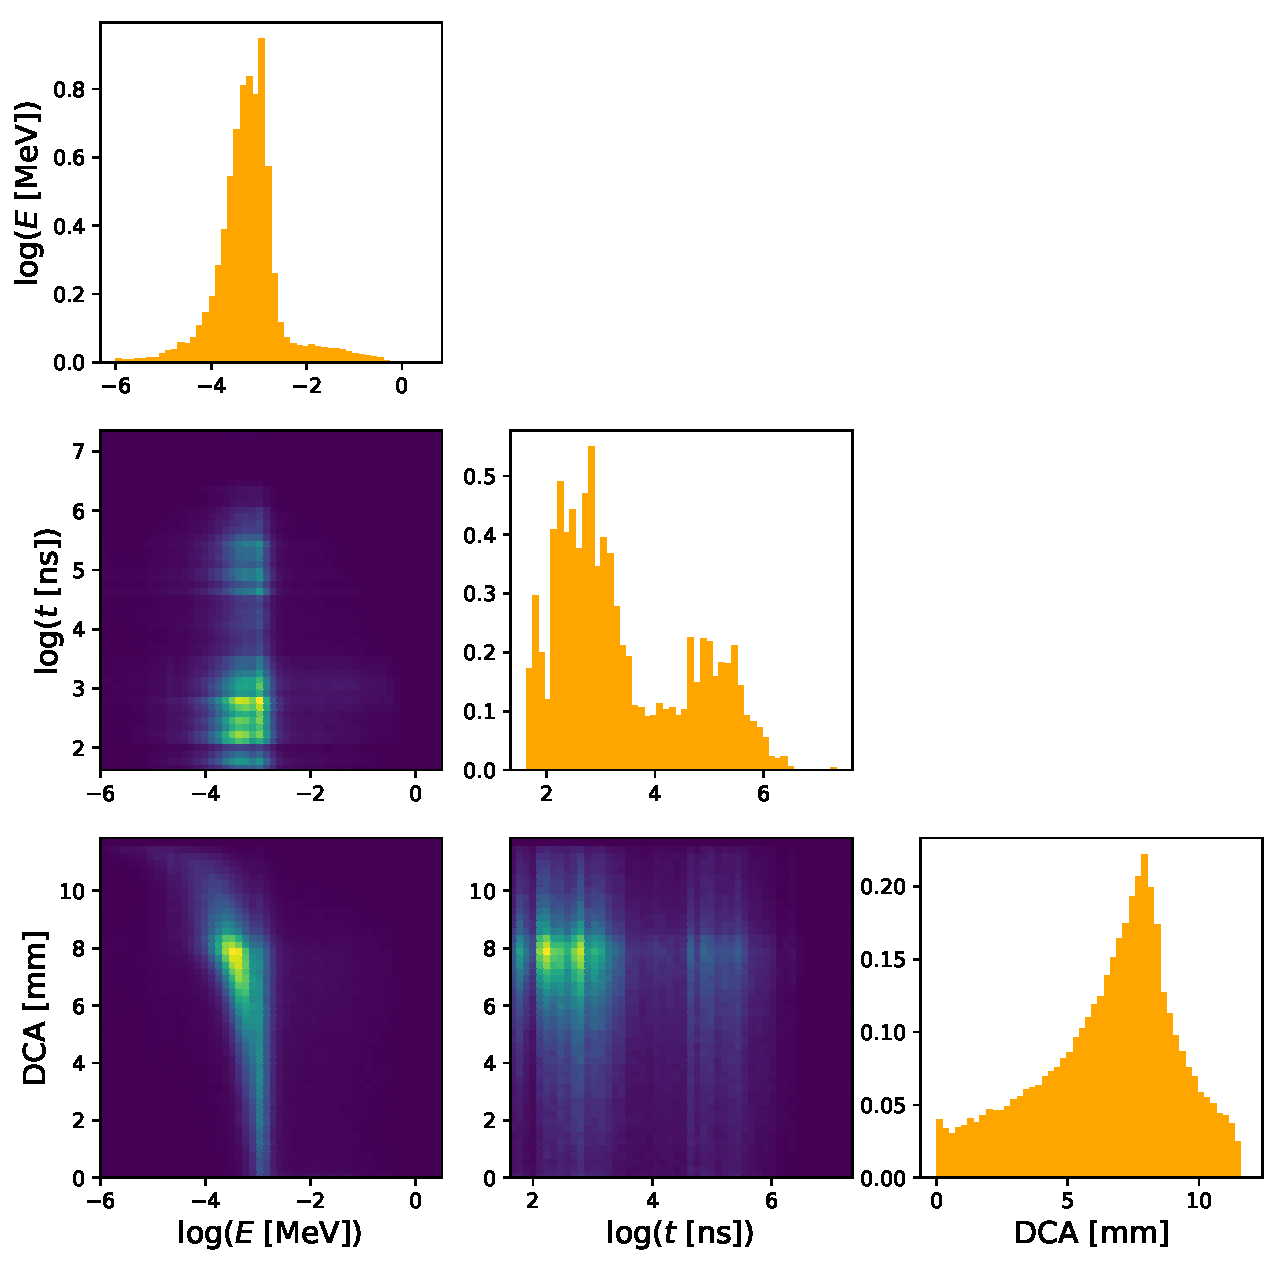
\includegraphics[width=\textwidth]{chapter4/feature_matrix_fake.pdf}
        \caption{GAN-generated dataset.}
    \end{subfigure}
    \caption{
        Comparison of feature distributions and correlations when generating a
        dataset of the same size as the training dataset.
    }
    \label{fig:comp_feature_distributions}
\end{figure}

% For KL div (P || Q) notation
\DeclarePairedDelimiterX{\infdivx}[2]{(}{)}{%
  #1\;\delimsize\|\;#2%
}


In order to summarise the similarity between the distribution of real and generated
samples into one quantity, a commonly used metric is the Kullback-Leibler (KL)
divergence which can be interpreted as the amount of information lost when
approximating the real dataset with a generated one~\cite{10.1214/aoms/1177729694}.
KL divergence is defined on a probability space $\mathcal{X}$ as
\begin{equation}\label{eq:kl_div}
D_\mathrm{KL} \infdivx{P}{Q} = \sum_{x \in \mathcal{X}} P(x) \log \frac{P(x)}{Q(x)},
\end{equation}
where in our case $P$ denotes the distribution of real hits and $Q$ that of
generated hits. To compute $D_\mathrm{KL}$, the three continuous features of
every hit are binned into a 3D histogram to approximate the probability density
functions $P$ and $Q$ and the sum in Equation~\ref{eq:kl_div} is a sum over all
(non-zero) bins. The \texttt{edep} and \texttt{t} features are log-transformed
such that the resulting histogram is smoother. Figure~\ref{fig:kl_div} shows the
Kullback-Leibler divergence between the continuous distributions of real and
generated hits over training iterations. For this specific model, the KL
divergence converges around 100 epochs.


\begin{figure}
    \centering
    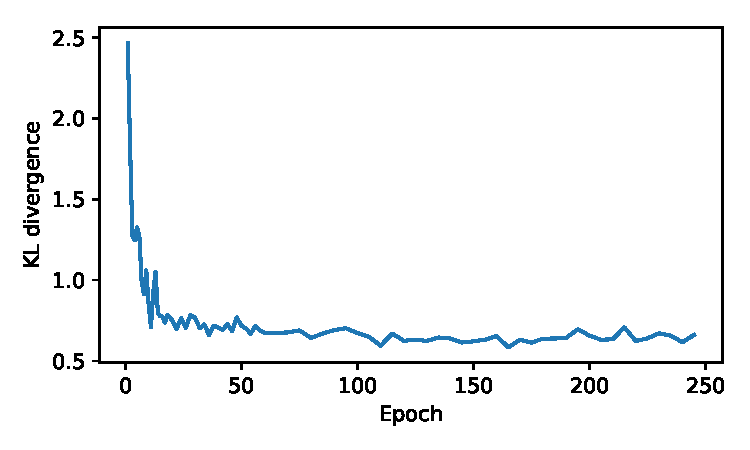
\includegraphics[width=0.5\textwidth]{chapter4/job_21175015_kldiv.pdf}
    \caption{Kullback-Leibler divergence between the distributions of real and generated hits as a function of training epochs.}
    \label{fig:kl_div}
\end{figure}

In addition to comparing the features that are given as input to the GAN for
training, we also examine quantities which are only present implicitly in the
training samples. Figure~\ref{fig:comp_nonlearned} shows a
comparison of the relative amounts of hits in each CDC layer and of the
``occupancy'' per sample, i.e.\ the fraction of wires on which a hit occurs.
This allows us to determine whether or not the model sees beyond the features
provided explicitly for training.

\begin{figure}
    \centering
    %\captionsetup[subfigure]{justification=centering}
    \begin{subfigure}[t]{0.38\textwidth}
        \centering
        \hspace{-.5cm} % To align graphics with caption
        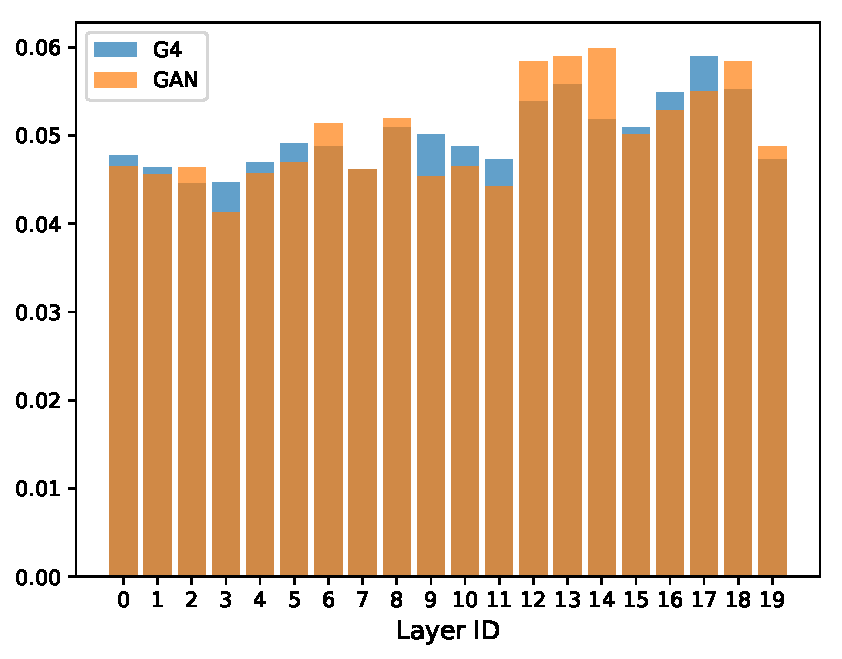
\includegraphics[width=\textwidth]{chapter4/comp_layer.pdf}
        \caption{Layer index, which is related to wire index and radial position.}
    \end{subfigure}
    \hspace{2cm}
    \begin{subfigure}[t]{0.38\textwidth}
        \centering
        \hspace{-.5cm} % To align graphics with caption
        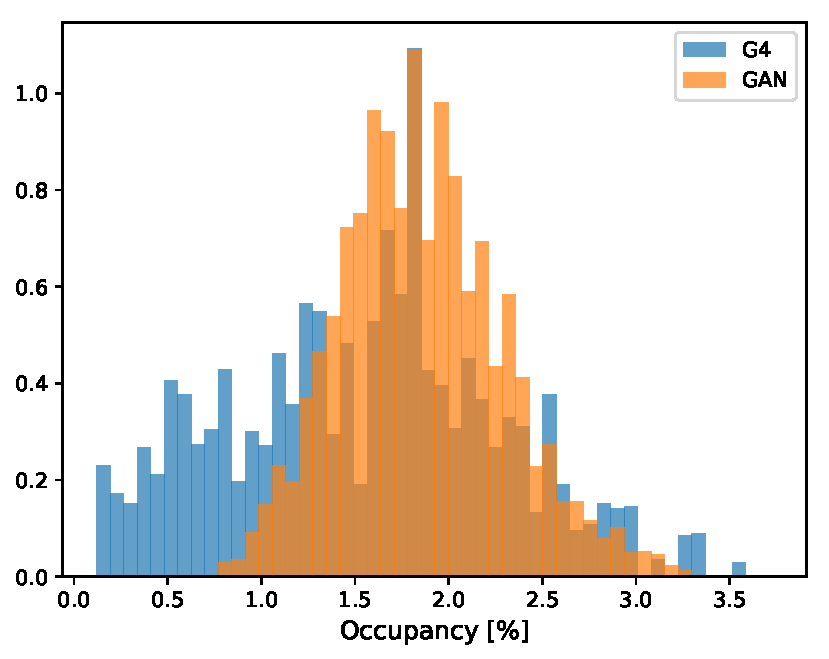
\includegraphics[width=\textwidth]{chapter4/occupancy.pdf}
        \caption{Occupancy, i.e.\ the number of activated wires in a given sequence.}
    \end{subfigure}
    \caption{
        Comparison of quantities not explicitly learned by the GAN model.
    }
    \label{fig:comp_nonlearned}
\end{figure}


\section{Quality metrics}\label{sec:quality_metrics} % FID, custom CNN, transfer learning w/ Inception-v3

The Kullback-Leibler divergence provides a metric to measure how close a
distribution of generated samples is to that of training samples. However, it
does not provide an indication of how closely individual generated samples
resemble real samples. 

For that, one method which is commonly used in the field
of GANs is an external classifier that can extract features from the generated
and real samples. These extracted features can then be used to understand the
differences between the two and why they arise.

The task of investigating the quality of generated hit samples from the CDC GAN
was tackled by a pair of Master's students during a six-month
project~\cite{noam, irene}. The following methods and results are the product of
their work.
% Three types of quality metrics were used to
% quantitatively evaluate samples and to understand more deeply the differences between
% the GAN's output and the MC data. 


\subsection{Inception score}

In image generation tasks, the \emph{Inception score} was proposed as a quality
metric to compare images generated by different GAN
models~\cite{salimans_improved_2016}. 
An Inception model~\cite{7298594}, trained independently on the ImageNet dataset
to classify images, is applied to GAN-generated images to obtain label
probabilities for each sample. The metric is then formulated in terms of the label
distribution to favour generated images which depict a specific object rather than
some average of classes, while disfavouring a generator whose images all resemble
the same class.

\subsection{Fréchet Inception Distance}

% $$
% \mathrm{Inception\ score} = \exp \mathrm{KL}(p(y|x)\ ||\ p(y)),
% $$
% where $\mathrm{KL}$ denotes the Kullback-Leibler divergence, $p(y|x)$ is the
% distribution of label probabilities assigned by the Inception network, and
% $p(y)$ is the marginal $p(y) = \int p(y|x = G(z)) \mathrm{d}z$.

The Fréchet Inception Distance (FID) is an evolution of the Inception score
which additionally uses statistics extracted from the training dataset to
estimate a distance between real and generated
samples~\cite{10.5555/3295222.3295408}. Conventionally, a pre-trained
Inception-v3 model~\cite{7780677} is applied to real and generated samples.
Activations from an intermediate layer are extracted and their mean $\bm{\mu}$
and covariance $\bm{\Sigma}$ are estimated, from which the Fréchet (or
Wasserstein-2) distance is calculated as
\begin{equation}
d^2 = | \bm{\mu}_G - \bm{\mu}_R |^2 + 
    \mathrm{Tr}(\bm{\Sigma}_G + \bm{\Sigma}_R - 
    2(\bm{\Sigma}_G \bm{\Sigma}_R)^{1/2})    
\end{equation}
where the $G$ and $R$ subscripts respectively denote generated and real statistics.

Applying these methods to domains other than image generation is not
straightforward because the Inception network used to compute the metric is
specific to raster images with three colour channels. This has prompted the
development of domain-specific metrics such as Fréchet Audio
Distance~\cite{kilgour19_interspeech} and Fréchet Video
Distance~\cite{Unterthiner2018TowardsAG}, as well as the Graph Fréchet Distance
used to evaluate particle jets generated by a graph-based GAN for LHC
experiments~\cite{kansal2020graph}.



\subsection{Evaluating the CDC GAN performance}

\subsubsection{Pre-trained Inception-v3}
As a baseline to evaluate the CDC GAN, the Inception-v3 model trained on the
ImageNet dataset was used to compute FID between generated and real samples. The
network expects images as input, i.e.\ tensors with two spatial dimensions and
three channels, which means our hit data must be arranged to fit this shape.

GAN-generated hits have three continuous features and a position. The three
features can simply be passed as analogues to the three colour channels, but the
hit positions must be discretised in order to get an image-like object. In
addition, the ordering of hits bears importance, so it ought to be considered as a
third, temporal dimension. However, Inception cannot process 3D objects hence a
solution is to project out one of the dimensions and compute three orthogonal
scores, one for each projection. Figure~\ref{fig:FID_vs_epochs} shows FID
computed for each of the three projections as a function of training iterations.


\begin{figure}
    \centering
    \begin{subfigure}[t]{0.32\textwidth}
        \centering
        \hspace{-0.85cm}
        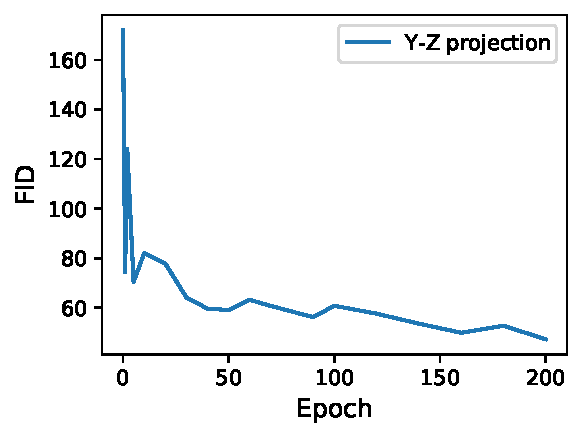
\includegraphics[width=\textwidth]{chapter4/fid_epoch-yz.pdf}
        %\caption{}
    \end{subfigure}
    \begin{subfigure}[t]{0.32\textwidth}
        \centering
        \hspace{-0.85cm}
        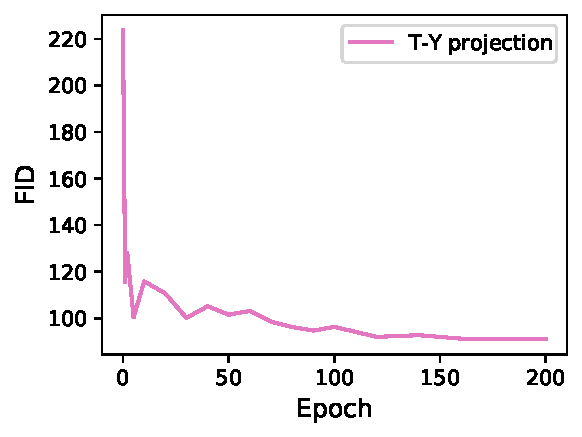
\includegraphics[width=\textwidth]{chapter4/fid_epoch-ty.pdf}
        %\caption{}
    \end{subfigure}
    \begin{subfigure}[t]{0.32\textwidth}
        \centering
        \hspace{-0.85cm}
        \includegraphics[width=\textwidth]{chapter4/fid_epoch-tz.pdf}
        %\caption{}
    \end{subfigure}
    \caption{ Fréchet Inception Distance computed by the pre-trained
        Inception-v3 network over training epochs of the CDC GAN. Since
        Inception requires a 2D image as input and our hit sequences have a
        third temporal dimension, the hit data is projected along its axes and
        a separate FID is calculated for each projection. }
    \label{fig:FID_vs_epochs}
\end{figure}

% Hit positions are discretised into a $300 \times 300$ grid and the three
% continuous features are used as channels. 

In order to process whole hit sequences rather than projections, two alternative
methods were considered: training a custom network which can take
three-dimensional tensors as input, and adding layers to the Inception network
so that it can more naturally process our hit data.

\subsubsection{3D convolutional neural network}

A custom neural network is developed to process whole hit sequences and compute a
domain-specific FID. The architecture is composed of four convolutional layers that
extract features from hit sequences, i.e.\ three-dimensional tensors with three
channels. The convolution kernels are thus themselves 3D, and strides help the
network extract features at different scales, as for the GAN critic.

The convolutional neural network (CNN) is trained to discriminate Monte Carlo
noise-like hit sequences from reconstructible ones. We expect such a classifier
to rely on the positioning and clustering of hit patterns to discriminate
samples. The intermediate activations which will be used to compute the Fréchet
distance ought to be a representation of that information and hence help to
define a sensible distance metric.

Once trained, the CNN reaches a classification accuracy of \SI{98.7}{\percent},
and it can be used to compute FID on GAN-generated samples.
Figure~\ref{fig:custom_distance_vs_epochs} shows FID over epochs of the CDC GAN
training.


\subsubsection{Transfer learning Inception-v3}

Transfer learning (TL) refers to the addition and subsequent training of layers
to a fixed pre-trained network in order to apply it to a new domain. By adding
layers to the front and back of Inception-v3, it can be adapted to the hit
sequence classification task. The weights in the new layers are adjusted to
discriminate noise-like from reconstructible hit sequences, which allows
domain-specific features to be extracted. In addition, because the input layer
is modified, this new network is made to provide a single FID score rather than
three to compare GAN-generated samples to real ones.
Figure~\ref{fig:transfer_learning_FID_vs_epochs} shows the resulting FID score
computed by the TL Inception-v3 over epochs of the CDC GAN training.

\begin{figure}
    \centering
    \begin{subfigure}[t]{0.4\textwidth}
        \centering
        \hspace{-1cm} % To align graphics with caption
        \includegraphics[width=\textwidth]{chapter4/cnn_fid-epoch.pdf}
        \caption{
            Domain-specific 3D CNN.
        }
        \label{fig:custom_distance_vs_epochs}
    \end{subfigure}
    \hfill
    \begin{subfigure}[t]{0.4\textwidth}
        \centering
        \hspace{-1cm} % To align graphics with caption
        \includegraphics[width=\textwidth]{chapter4/tr_learning-epoch.pdf}
        \caption{ 
            Transfer Learning Inception-v3.
        }
        \label{fig:transfer_learning_FID_vs_epochs}
    \end{subfigure}
    \caption{
        Fréchet Inception Distance computed over training epochs of the CDC GAN
        by two external neural networks. Unlike in
        Figure~\ref{fig:FID_vs_epochs}, hit sequences can be processed at once
        without projecting them along an axis. The 3D CNN is trained on
        Monte Carlo hit data, in the same way as the front and back layers added
        to Inception-v3 for transfer learning.
    }
\end{figure}

\subsection{Interpretation of FID}
The Fréchet Inception Distance is a single quantity whose value indicates how
similar generated samples are to real samples. It summarises the statistics of
features extracted by an external neural network, but it does not directly show
which features seem different.

We could also plot the feature vectors directly and determine where their
distributions differ between real and fake samples, however the vectors have a
high dimensionality and cannot be easily visualised. The solution that was
adopted is to use the Uniform Manifold Approximation and Projection
(UMAP)~\cite{umap} method to optimally project the feature vectors onto two
dimensions. Each sample can then be associated with a single point in a 2D space
and thus one can more easily visualise the distribution of samples. 

Figure~\ref{fig:umap} shows a UMAP plot of generated and real samples, including
reconstructible hit sequences. The position of each point is a projection of the
feature vector extracted from each sample by the transfer learning Inception-v3
network. Such a plot shows that reconstructible and noise-like sequences are
adequately discriminated by the network, and that the generated and noise-like
sequences overlap in large part. Hence, the GAN is clearly able to produce
samples which resemble the training dataset. However, some portion of the space
covered by noise-like MC samples is not occupied by any generated samples, which
indicates that the GAN cannot produce these types of samples.

By tracing UMAP points back to the sample they were computed from, one can then
attempt to understand the type of sample which the GAN cannot faithfully
produce. This yields insight into the GAN's strategy and where exactly it fails
to perform, which subsequently helps to adjust its design and architecture.


\begin{figure}
    \centering
    \includegraphics[width=0.4\textwidth]{chapter4/umap_TL_fid_singlefit.pdf}
    \caption{ UMAP computed from feature vectors extracted by the TL
        Inception-v3 network, for reconstructible, noise-like and generated hit
        sequences. The number of neighbours in the UMAP transform was set to
        50. }
    \label{fig:umap}
\end{figure}



% The hit generation rate is X hits/s, whereas a traditional MC simulation
% starting from the POT collision creates X hits/s. If re-seeding is used to
% sample particles at the detector region boundary, X hits/s can be produced, so
% the efficiency gain is about 1e7. However the worry is not so much whether or
% not GANs can yield increase in efficiency (they can), but whether their output
% respects all the physical properties expected from MC data.

%\subsection{\hl{How GAN-generated hits are merged back into a dataset}}
\chapter{Backward Monte Carlo simulation for cosmic ray events}\label{ch:cosmics}

\begin{markdown}

1. Intro to BMC: relation to adjoint MC (find refs), maybe diagram

2. Physics: how we use BMC to determine rates of cosmic events: equations for
flux, sampling PDF, BMC weights, topography map of J-PARC

3. Integration into ICEDUST: implementation of sampling methods, event loop, output to
oaRooTracker format
+ `https://gitlab.in2p3.fr/comet/ICEDUST_packages/-/merge_requests/534`
+ `https://gitlab.in2p3.fr/comet/ICEDUST_packages/-/wikis/Backward-Monte-Carlo-sampling-with-SimBackwardMC#rate-calculation`

3. Actual estimation of background rate in Phase-I, maybe just quoting V's
result


\end{markdown}

% Intro: cosmics are important
Cosmic ray-induced events represent a significant part of the expected
background in the COMET experiment, as discussed in
Section~\ref{sec:backgrounds}. Cosmic muons irradiate the Earth at irregular
intervals and have a wide energy range, hence some fraction of them will be able
to mimic the conversion signal by entering the COMET detector system. 

Estimating the rate at which cosmic muons might produce signal-like events is
computationally expensive through standard Monte Carlo simulation methods. This
is due to the fact that the source of cosmic muons, i.e.\ the atmosphere, has a
much greater spatial extent than the active detector region. Hence, most cosmic
events generated from an atmospheric source will miss the detector completely
and not contribute in the estimation of the background rate, resulting in wasted
computation time.

A reverse (or adjoint) Monte Carlo simulation is one where the flow of particle
transport is reversed, i.e.\ events are generated in the sensitive detector
volume and propagated backward in time until they reach the source. This method
was initially used in 1967 to estimate gamma-ray and neutron radiation doses in
nuclear reactors~\cite{doi:10.13182/NSE68-A19235,doi:10.13182/NSE69-A19116}.
More recently, reverse MC has also been integrated into Geant4
simulations~\cite{DESORGHER2010247} for dosimetry in space, reversing the
electromagnetic physics of electrons, protons and ions.

In the case of muons, a backward transport method was developed by Niess et
al.~\cite{Niess_Barnoud_Carloganu_Menedeu_2018} in the context of muon
tomography, and it was later adapted to the COMET experiment in order to refine
estimations of the background rate from cosmic rays. This chapter discusses the
backward MC method for cosmic muons, how it is applied to COMET and the
resulting rate estimations in COMET Phase-I.


\section{Backward Monte Carlo transport}
In standard Monte Carlo simulations, events are generated by a source and
propagated forward in time according to their equations of motion and
interaction cross-sections within any surrounding medium. In a situation where
the source is large compared to the sensitive detector volume, as illustrated in
Figure~\ref{fig:bmc_configuration}, events have a high probability to miss the
detector and contribute nothing in the desired computation.

In backward MC, events are generated according to an arbitrary probability
density function (PDF) around the detector volume. The overall sampling PDF is
typically the composite of a position, direction and energy sampling
distributions, i.e.\ 
$$
p(\bm{x}, \bm{p}, E) = p(\bm{x}) \times p(\bm{p}) \times p(E),
$$
where $p$ denotes a PDF whose integral is 1, $\bm{x}$ denotes position, $\bm{p}$
direction and $E$ energy. 

\sepfootnotecontent{A}{See Reference~\cite{DESORGHER2010247} for a thorough
discussion of adjoint cross-sections, weights, weight corrections and source
normalisation.}

Each event is propagated backward using adjoint transport and interaction
kernels such that the probability of the event can eventually be determined. At
each step of the propagation, a multiplicative weight is computed from the
adjoint interaction cross-sections in the local medium. When the particle
reaches the source, the directional flux at the source is used as a
normalisation factor to yield the final event weight\sepfootnote{A}. Given a
significant enough sample of reverse events, the weights can be summed to
obtain the absolute flux or rate of particles hitting the detector.


% Interesting paragraph from desorgher:
%  The Monte Carlo sampling of a big enough number of reverse tracks is
%  equivalent to the integration of the weight W over all independent variable
%  (E1,O1,Sd,x1,E0, ...) summed over all type of reverse reactions, atomic
%  elements, adjoint primaries, and adjoint secondaries. In this integration the
%  cases where more than one reaction and no reaction occur are also considered
%  and only the tracks reaching the external source are accounted for. By this
%  way the same answer is obtained as in the forward case.

\begin{figure}
    \centering
    %\includegraphics[width=0.6\textwidth]{chapter5/qwe.png}
    \caption{BMC configuration.}
    \label{fig:bmc_configuration}
\end{figure}

% How does one estimate the rate of cosmics from the sampling PDF and BMC
% weights?
% Describe procedure / maths?

% We backward propagate the same event many times in order to get a reasonable
% rate estimate. Perhaps mention that.

\section{Cosmic muon rate estimation}
% Here, talk about the COMET setup: 
% + We want to estimate the rate of background events caused by 
%   muons+secondaries hitting the detector
% + Thus, we sample muons+/- around the envelope of the CRV, according to [spell
%   out PDF]
% + We apply backward MC up to an atmospheric muon flux model at altitude X,
%   tabulated from CORSIKA etc.
% + We can first estimate the cosmic muon rate on each surface of the CRV
%   Show plots etc.
% + From the events generated at the CRV envelope, it is also possible to
%   propagate forward to determine which events might produce signal-like
%   tracks.
% + Once this is done, we use the results from backward propagation to estimate
%   rate of background-inducing cosmic muons, qed.


% Do we talk about the PUMAS, GOUPIL setup?
% ICEDUST integration?
\chapter{COMET Phase-I sensitivity and backgrounds}

With the framework to simulate backgrounds from atmospheric muons in place, we
can now combine the results into a complete sensitivity and background
simulation study for COMET Phase-I. In this chapter, we discuss our simulation
samples consisting of signal, decay in orbit (DIO), and atmospheric events, and
present our resulting expectations of the performance of Phase-I.

\section{Simulation setup}
Three simulation samples are produced for this study. A $\mu$--$e$ conversion
sample, a DIO sample and an atmospheric muon sample. All three are simulated in
the geometrical world shown in Figure~\ref{fig:bmc_geometry}. This geometry
differs from the older TDR design~\cite{the_comet_collaboration_comet_2020} by
the number of counters in the CTH. Here, each layer of the CTH has 64 counters
instead of the original 48, which mainly affects the detector's geometrical
acceptance. In addition, the outer layer of the CTH is composed of plastic
scintillator counters rather than the Cherenkov counters, as was originally
planned. As we will see, this has an important effect on the detector's ability
to discriminate atmospheric anti-muons from conversion electrons.

\subsection{\texorpdfstring{$\mu$--$e$}{Muon to electron} conversion} 

\subsubsection{Sample}

The signal sample is the most straightforward to produce. We initially generate
primary electrons with energy $E=\SI{104.97}{\MeV}$ uniformly inside the
stopping target disks. Their direction is isotropically distributed, as would be
the case in the conversion process. A uniform position distribution in each disk
is not realistic, because the actual distribution depends on where in the
stopping target the muons in the beam become bound. To account for this, the
events are weighted according to the stopping positions of muons recorded in the
MC5 simulation. The weighting factor is determined from the relative probability
for a muon to stop at the sampled position, which is estimated by histogramming
the stopping positions in each disk.
Figure~\ref{fig:stopping_position_reweighting} shows the sampled uniform
position distribution and the resulting distribution after weighting. In total,
$N_\mathrm{signal} = 2\times 10^6$ events are simulated to compose the signal
sample.

% After applying geom cut of CTH trigger, how many remain?

\begin{figure}
    \centering
    \begin{subfigure}{0.46\textwidth}
        \centering
        \caption{Pre-weighting.}
    \end{subfigure}
    \hfill
    \begin{subfigure}{0.46\textwidth}
        \centering
        \caption{Post-weighting.}
    \end{subfigure}
    \caption{ Initial position distribution of signal electrons before and after
        weighting them by the likelihood of a muon being bound in each bin. }
    \label{fig:stopping_position_reweighting}
\end{figure}

\begin{figure}
    \centering
    
    \caption{Conversion signal event in the CyDet system.}
    \label{fig:signal_in_cydet}
\end{figure}

\subsubsection{Selection}
Signal events are selected based on detector acceptance criteria. We first require
fourfold coincidence in the CTH. The fraction of events remaining
defines the geometrical acceptance 
$$
A_\mathrm{geom} \equiv  \frac{\text{fourfold coincidences}}{N_\mathrm{signal}}.
$$
In our simulation setup with the 64-counters-per-layer CTH, our estimated
geometrical acceptance is $A_\mathrm{geom} = \SI{21}{\percent}$. In comparison,
the TDR cites $A_\mathrm{geom} = \SI{26}{\percent}$ with the previous design of
the CTH. 
\hl{Figure~X shows a conversion event which passes the
fourfold coincidence selection criterion.??}

% Reconstruction
We do not fully simulate the reconstruction of signal electron trajectories in
the CDC. In order to approximate the effect of reconstruction uncertainties, a
smearing is applied to the true momentum of each track. The reconstructed
momentum is estimated as $p_r = p_t + x$, where $p_t$ is the true momentum of
the electron as it enters the CDC, $x \sim \mathcal{N}(0, \sigma)$, and $\sigma
= \SI{200}{\keV/\clight}$ is the expected momentum resolution of the CDC.

% Other acceptance factors (not simulated)
Other acceptance criteria, such as the trigger timing window and reconstruction
quality cuts, are not properly simulated in this study. Instead, we apply
efficiency factors for each of them based on their TDR estimates.
\hl{Reference a table here?}


\subsection{Muon decay in orbit}
\subsubsection{Sample}
The DIO sample is similar to the signal sample in that the initial position
of signal and DIO electrons is identically distributed. Hence, we also sample
uniformly in the stopping target disks and then weight the events according to
the MC5 stopping position distribution. Similarly, the direction of DIO
electrons is sampled isotropically. The energy distribution is thus the only
difference between the two samples. 

\begin{figure}
    \centering
    
    \caption{Energy spectrum of DIO electrons from muonic aluminium atoms.}
    \label{fig:czarnecki_spectrum}
\end{figure}

The theoretical energy spectrum of DIO electrons produced in aluminium muonic
atoms was determined by Czarnecki et al.~\cite{czarnecki} and is shown in
Figure~\ref{fig:czarnecki_spectrum}. Their calculated spectrum is used to
determine an energy weighting factor for simulated DIO events. In a similar way
to the position weighting procedure, DIO events are first generated with a
uniform energy distribution, and then weighted according to the relative
likelihood for a DIO electron to have the sampled energy.
Figure~\ref{fig:dio_energy_reweighting} shows the weighted energy distribution
compared to the theoretical energy spectrum. \hl{FIGURE and then adjust text}.
The DIO sample is composed of $N_\mathrm{DIO} = 10^7$ events in total.

\begin{figure}
    \centering
    
    \caption{DIO-induced background with momentum  $p=\SI{1}{\MeV/\clight}$.}
    \label{fig:muon_dio_in_cydet}
\end{figure}

\subsubsection{Selection}
The selection of DIO events is identical to the selection of conversion events.
We require a fourfold coincidence in the CTH, and then apply a Gaussian smear to
the true momentum of the electron to simulate track reconstruction. The same
efficiency factors as for signal events are applied.

\subsection{Atmospheric muons}

\subsubsection{Sample}

Atmospheric muon events are simulated as explained in
Section~\ref{sec:cosmic_event_sampling}. Two samples are produced, one on the
entire surface of the CRV and one more densely concentrated on its upstream and
downstream openings. Because of how rarely a sampled atmospheric event produces
signal-like features, the atmospheric dataset is by far the largest of the
three, with $1 \times 10^9$ events generated on the envelope and $1.4 \times
10^9$ on the openings.



\begin{figure}
    \centering
    
    \caption{Cosmic ray-induced background with momentum $p=\SI{1}{\MeV/\clight}$.}
    \label{fig:cosmic_bg_in_cydet}
\end{figure}


\hl{TODO remove below}

The time distribution of signal, DIO and atmospheric events is not realistically
simulated in this study. Instead, we apply an average timing window efficiency
factor to all events in order to estimate the total count integrated over
data-acquisition time.

The time efficiency factor is not the same for signal, DIO and cosmics,
because they don't have the same time distribution. For cosmics, the time
distribution is ~uniform, so the factor should just be live time / (live +
dead time). For signal and DIO, it is dependent upon the time distribution of
muon bound in the tgt.

\subsubsection{Selection}
\hl{TODO}


\subsection{Sample weighting}
\sepfootnotecontent{fn:conv_br_norm}{The nuclear muon capture branching ratio appears in this
expression because the branching ratio of $\mu$--$e$ conversion is
conventionally normalised to $\mathcal{B}_\mathrm{capture}$.}

Because they originate from different processes, the three MC samples must be
weighted differently in order to determine the absolute contribution from each.
The conversion and DIO processes both originate from the muons bound in the
stopping target, hence we can express the total number of expected conversion
and DIO electrons in terms of the total number of stopped muons $N_\mu$.
The number of signal electrons, as a function of the conversion branching
ratio $\mathcal{B}_\mathrm{conversion}$, is:
$$
N_{e^-}^\mathrm{conversion} = 
N_\mu \, \mathcal{B}_\mathrm{conversion} \, 
\mathcal{B}_\mathrm{capture} \, f_\mathrm{coherent},
$$
where $\mathcal{B}_\mathrm{capture} = 0.61$ is the branching ratio of nuclear
muon capture\sepfootnote{fn:conv_br_norm} and $f_\mathrm{coherent}=0.9$ is the
fraction of conversions that are coherent. Similarly, the total number of DIO
electrons can be expressed as:
$$
N_{e^-}^\mathrm{DIO} = N_\mu \, \mathcal{B}_\mathrm{DIO},
$$
where $\mathcal{B}_\mathrm{DIO} = 1 - \mathcal{B}_\mathrm{capture} -
\mathcal{B}_\mathrm{conversion} \approx 0.39$ is the branching ratio of DIO.


In the case of atmospheric muons, the backward MC procedure yields an absolute
rate. This rate is multiplied by the total data acquisition (DAQ) time of the
experiment to obtain the expected background count:
$$
N_\mathrm{atmospheric} = R \times T_\mathrm{DAQ},
$$
where $R$ is the total atmospheric background rate, and we set
$T_\mathrm{DAQ}=146$ days, corresponding to $N_\mu = 1.5\times 10^{19}$, in this
study. 

\subsubsection{Trigger time window efficiencies}
In order to take into account the trigger timing window, we assume that
atmospheric muons irradiate the detector with a uniform time distribution.
Hence, the time window efficiency factor is simply the average fraction of
time when the trigger is active:
$$
\epsilon_\text{time window}^\mathrm{atmospheric} =
\frac{8}{9}\,\frac{1170 - 700}{1170} = \SI{36}{\percent}
$$
assuming the trigger window is between 700 and \SI{1170}{\ns}, and where the
factor $\frac{8}{9}$ arises from the bunch structure of the J-PARC main ring. In
contrast, the efficiency factor for conversion and DIO electrons
$\epsilon_\text{time window}^\text{conversion|DIO} \approx \SI{30}{\percent}$ is
smaller because the time distribution of bound muons peaks around \SI{300}{\ns},
before the trigger becomes active (see Figure~\ref{fig:timing_distributions}).



\section{Single event sensitivity}
The single event sensitivity (SES) is defined as the value of the $\mu$--$e$
conversion branching ratio required for the experiment to observe one signal
event. It can be expressed in terms of the experimental acceptance $A_{\mu-e}$ and the
total number of muons stopped in the stopping target $N_\mu$:
\begin{equation}
    \mathrm{SES} = \frac{1}{N_\mu\,A_{\mu-e}\,\mathcal{B}_\mathrm{capture}\,f_\mathrm{coherent}},
\end{equation}
where $\mathcal{B}_\mathrm{capture} = 0.61$ is the branching ratio of nuclear
muon capture and $f_\mathrm{coherent} = 0.9$ is the fraction of conversions
expected to leave the nucleus in its ground state.

% Is it worth ELI5 here?
% The net signal acceptance $A_{\mu-e}$ is the product of various factors stemming
% from the experiment's design and inefficiencies in the processing,
% reconstruction and selection of candidate events. 

% How do we approach the fact that CTH geom has changed so our geom acceptance
% is lower?

\hl{ v We've already mentioned trigger selection and acceptance in the Selection
    subsec of every sample. Cut.}
    
In this study, the CTH trigger mechanism was simulated by finding events
involving a fourfold coincidence. The fraction of signal events which induce a
trigger is defined as the geometrical acceptance $A_\mathrm{geom}$. In our
simulation setup, the CTH contains 64 counters per layer, two layers
in each module, one module at the upstream end of the CDC and the other
downstream (256 counters in total). Our estimated geometrical acceptance is
$$
A_\mathrm{geom} \equiv \frac{\text{fourfold coincidences}}{N_\mathrm{signal}} = \SI{21}{\percent}.
$$
In comparison, the COMET Phase-I TDR~\cite{the_comet_collaboration_comet_2020}
cites $A_\mathrm{geom} = \SI{26}{\percent}$ with the previous design of the CTH,
which had 48 counters per layer. This reduced acceptance worsens the sensitivity
of the experiment slightly. In this study, none of the other experimental
aspects that contribute to the net acceptance were changed, hence we use the
other factors of $A_{\mu-e}$ from the TDR, and only replace the value of
$A_\mathrm{geom}$ with the newly estimated one. Values of the acceptance
coefficients used in our study are shown in Table~\ref{tab:acceptance}. The net
signal acceptance using these factors is $A_{\mu-e} = 0.032$.

The number of muons stopped in the stopping target, $N_\mu$, is a function of
the COMET beam power, the target material, the design of the
transport system, and the total data-acquisition time. 
The target material sets the yield of
backward-going pions which will decay to muons of the right momentum to come at
rest in the muon stopping target. This, combined with the transport system,
determines the yield of stopped muons per proton collision $R_{\mu/p} \equiv
\frac{\text{muons stopped}}{\text{proton on target}}$. Here, we use the
MC5 dataset, a sample of $10^9$ POT collisions, to estimate $R_{\mu/p}=4.86
\times 10^{-4}$.
The beam power and data-acquisition time together determine the total number of proton
collisions that will occur. COMET Phase-I requires $N_\mathrm{POT} = 3.15 \times
10^{19}$ collisions in order to reach its sensitivity goal, corresponding to a
data-acquisition time of $T=146$ days.
These figures allow us to estimate the total number of stopped muons
$$N_\mu = R_{\mu/p} \times N_\mathrm{POT} = 1.56\times 10^{16},$$
which can be substituted into the SES formula:
\begin{equation}\label{eq:my_ses}
\mathrm{SES}
=\frac{1}{N_\mu\,A_{\mu-e}\,\mathcal{B}_\mathrm{capture}\,f_\mathrm{coherent}}
= 3.81\times10^{-15}.
\end{equation}
This value is slightly worse than the TDR estimation,
$\mathrm{SES}_\mathrm{TDR}=3\times 10^{-15}$, because of our lower geometrical
acceptance when using the new CTH design.

% \begin{table}
%     \centering\begin{tabular}{l|ccc}
%         \toprule
%         a&b&c&d\\\midrule
%         a&b&c&d\\
%         \bottomrule
%     \end{tabular}
%     \caption{ Acceptance coefficients used to estimate the single event
%     sensitivity in Equation~\ref{eq:my_ses}. These also apply to the
%     decay-in-orbit background rate estimation. }
%     \label{tab:ses_efficiency_factors}
% \end{table}


\section{Momentum spectra}
Because the signal has a clear mono-energetic signature, a precise measurement
of the momentum of candidate tracks helps to discriminate signal from
backgrounds. Figure~\ref{fig:log_spectrum} shows the momentum spectrum
for candidate conversion, DIO and atmospheric events.

\begin{figure}
    \centering
    
    \caption{Log spectrum.}
    \label{fig:log_spectrum}
\end{figure}

\section{Discussion}

\subsection{Atmospheric $\mu^+$ backgrounds}

\subsection{CRV efficiency}

\subsection{Particle identification}


\chapter{Conclusion}

% Muon and LFV
Since the discovery of the muon in 1937, our understanding of its properties has
been steadily evolving. Today, although it fits nicely into the Standard Model
of particle physics, some questions remain standing, and recent tensions
observed between theory and experiment are suggesting that the SM does not give
a complete picture of the muon's underlying nature. Charged lepton flavour
violation is one of the ways in which Nature might deviate from the SM. If CLFV
were observed, it would be a clear indication of new physics. Neutrino-less
muon-to-electron conversion is one of the most sensitive channels to search for
CLFV as its signature is a mono-energetic electron with few sources of potential
backgrounds. According to theoretical constraints, this process ought to be
suppressed beyond experimental sensitivities. Therefore, any observation of the
$\mu$--$e$ conversion signal would yield clear evidence for CLFV and hence guide
the field toward a better understanding of physics beyond the Standard Model.

% COMET
The COMET Phase\nobreakdash-I experiment will soon start its data acquisition
run toward the search for muon-to-electron conversion in aluminium. It is
expected to be a hundred times more sensitive to $\mu$--$e$ conversion than the
previous best measurement by SINDRUM II. To achieve this sensitivity, COMET
Phase\nobreakdash-I will produce an intense pulsed muon beam directed toward an
aluminium target to create muonic aluminium atoms, from which conversion
electrons may emerge. The Cylindrical Detector, which surrounds the muon
stopping target, is designed to clearly identify conversion electrons while
rejecting as many experimental backgrounds as possible. 

% Software & sim
In order to cover the needs of the experiment in terms of simulation,
calibration, reconstruction, data formats and data analysis, the COMET
collaboration develops a comprehensive set of software utilities named ICEDUST.
The work presented throughout this thesis relies heavily on Monte Carlo (MC) data
produced by ICEDUST's {\sc Geant4} simulations of Phase\nobreakdash-I.
% Here is a good place to kind of introduce the problem of producing large-scale
% datasets and estimating atmospheric backgrounds
MC simulations allow us to study the experiment outcomes and to optimise its
design before assembly. However, they are computationally expensive and
typically only allow us to simulate a small fraction of the amount of data
expected to be collected. Additionally, traditional MC sampling is particularly
inefficient when the source of events is far from the detector system, as is the
case when considering cosmic ray-induced backgrounds. This thesis aims to
address these two limitations by partially circumventing the brute force MC
method.

% GAN
We investigate a novel approach to the mass-production of simulation data based
on Generative Adversarial Networks. We propose a neural network generator of
hits for the Cylindrical Drift Chamber, which can produce synthetic energy
deposits in the detector at a rate $10^6$ times higher than the ICEDUST
simulation. The machine learning model is trained on a sample of simulated hits
and learns from their features and relationships. The trained model allows us to
generate only a subset of the hits produced by MC simulation, but far more
efficiently than was previously achievable. Our ambition for this work and
future developments is to enable the production of entire mock datasets, which
can be used by the collaboration in anticipation of data acquisition runs.

% BMC & background study
Additionally, we present a study of the backgrounds caused by cosmic ray-induced
atmospheric muons in the COMET Phase\nobreakdash-I muon-to-electron conversion search. We
use a backward Monte Carlo simulation method to efficiently estimate the flux of
atmospheric muons near the detector system. We then perform a full analysis of
the event count contributions from $\mu$--$e$ conversion, muon decay-in-orbit,
and atmospheric muons. Our findings suggest that an efficient rejection of
atmospheric backgrounds by the Cosmic Ray Veto, combined with particle-type
identification by the Cylindrical Detector, are necessary for the Phase\nobreakdash-I search
to succeed. Under optimistic conditions, namely with a
\SI{99.99}{\percent}-efficient CRV and \SI{99}{\percent} muon identification
rate by the CyDet, we expect 0.08 atmospheric background events during the 146
days of data acquisition. According to our analysis, during this run time, COMET
Phase\nobreakdash-I will be able to achieve a single event sensitivity of $3.61 \times
10^{-15}$.


% Wrap up: what do my results mean for COMET!!!
Our most important contributions have been integrated into the main ICEDUST
software repository and documented for others to use and build upon. As the
COMET experiment goes into the Phase\nobreakdash-I measurement period, we hope that these
techniques will help to refine our understanding of the data and that they can
be applied in preparation for Phase\nobreakdash-II and beyond.

\clearpage
\appendix
\chapter{Integration of backward Monte Carlo software into
ICEDUST}
\label{app:bmc_integration}

% \begin{itemize}
%     \item External packages: PUMAS, GOUPIL, GOUPIL components. Cite~\cite{NIESS2022108438}.
%     \item Internal package: SimBackwardMC
% \end{itemize}


\section{Original implementation}
The backward Monte Carlo simulation software was originally written and applied
to the COMET Phase\nobreakdash-I experiment by Valentin Niess, author
of~\cite{Niess_Barnoud_Carloganu_Menedeu_2018,NIESS2022108438}.
Figure~\ref{fig:pumas_integration_strategy} shows the layout of the original set
of software layers used to run backward MC simulations in the Phase\nobreakdash-I world. 

At the core of the backward Monte Carlo simulation is the backward transport
engine, PUMAS~\cite{NIESS2022108438}. PUMAS is responsible for the propagation
of particles through matter and the computation of MC weights based on the path
taken and the interactions undergone, as discussed in
Section~\ref{sec:bmc_method}. Because it is designed exclusively for this
purpose, PUMAS does not provide utilities for navigating through complex
geometries or sampling the flux from pre-computed tables. Another package,
GOUPIL, takes on this role as an interface to PUMAS, and allows the user to
specify a geometry, a source flux, as well as the local topography and
geomagnetic field around the experiment's location. An additional interface
between GOUPIL and {\sc Geant4}, \texttt{goupil-geant4}, was developed to allow
the user to control backward MC runs with the {\sc Geant4} macro user interface
and to load and navigate the geometry from a GDML file. The final layer,
\texttt{resample-simg4}, provides a command-line interface and enables events
generated by \texttt{SimG4} to be read as input for the backward MC simulation
to estimate their flux.


\begin{figure}
    \centering
    \includegraphics[width=0.6\textwidth]{appendixA/integration_strategy.drawio.pdf}
    \caption{ Software packages that compose the original backward MC simulation
        stack for the Phase\nobreakdash-I study, and organisation of their integrated
        ICEDUST counterparts.}
    \label{fig:pumas_integration_strategy}
\end{figure}

\section{Integration}

Figure~\ref{fig:pumas_integration_strategy} also shows how the original software
was arranged to become part of the ICEDUST framework. Since the PUMAS and GOUPIL
packages are unlikely to undergo quick iterative changes over time, they are integrated
into an external package. The functionalities of the upper two layers of the
stack are combined into a new ICEDUST package called \texttt{SimBackwardMC}.

The way in which the layers are organised is not the only difference between the
original and current software. Three major changes were implemented during the
integration in order to bring the original software closer to the ICEDUST
workflow.

\begin{itemize}
    \item {\bfseries Geometry format:} originally read from GDML files, the
    geometry is now created from the same classes and macro files that define
    the simulation world in forward MC runs by the \texttt{SimG4} package. This
    additionally ensures that the geometry used in forward and backward MC
    simulations is identical.
    \item {\bfseries Entry point:} the main \texttt{resample-simg4} entry point
    was previously a Lua script executed via LuaJIT which defined the
    command-line interface, configured the backward simulation run, and
    processed the output. \texttt{SimBackwardMC} uses a standard ICEDUST event
    loop executable as its entry point to handle command-line arguments, read
    events from input \texttt{oaEvent} files and output the results of the
    backward simulation.
    \item {\bfseries Output format:} \texttt{resample-simg4} wrote the results
    of backward sampling to a text file in a format similar to CSV.
    \texttt{SimBackwardMC} writes to a \texttt{RooTracker} file instead, since
    that is a standard ICEDUST format and a good fit to store the kinematics of
    processed events along with their estimated flux.
\end{itemize}

The integrated backward MC software presented here was used to obtain the
results of Chapters~\ref{ch:cosmics} and~\ref{ch:phase-I_study}. It is also
currently being used in the work of others, for instance to estimate the
atmospheric muon flux at various locations around the Phase\nobreakdash-I detector system
and validate the results with real measurements. Through our standardisation of
some parts of the original software and the addition of specific documentation,
we hope that the \texttt{SimBackwardMC} package will remain a readily accessible
tool for future cosmic ray studies in COMET.


\printbibliography

\listoffigures
\listoftables

\end{document}
